%==============================================================================
% tento soubor pouzijte jako zaklad
% this file should be used as a base for the thesis
% Autoři / Authors: 2008 Michal Bidlo, 2019 Jaroslav Dytrych
% Kontakt pro dotazy a připomínky: sablona@fit.vutbr.cz
% Contact for questions and comments: sablona@fit.vutbr.cz
%==============================================================================
% kodovani: UTF-8 (zmena prikazem iconv, recode nebo cstocs)
% encoding: UTF-8 (you can change it by command iconv, recode or cstocs)
%------------------------------------------------------------------------------
% zpracování / processing: make, make pdf, make clean
%==============================================================================
% Soubory, které je nutné upravit nebo smazat: / Files which have to be edited or deleted:
%   projekt-20-literatura-bibliography.bib - literatura / bibliography
%   projekt-01-kapitoly-chapters.tex - obsah práce / the thesis content
%   projekt-01-kapitoly-chapters-en.tex - obsah práce v angličtině / the thesis content in English
%   projekt-30-prilohy-appendices.tex - přílohy / appendices
%   projekt-30-prilohy-appendices-en.tex - přílohy v angličtině / appendices in English
%==============================================================================
%\documentclass[]{fitthesis} % bez zadání - pro začátek práce, aby nebyl problém s překladem
%\documentclass[english]{fitthesis} % without assignment - for the work start to avoid compilation problem
\documentclass[zadani]{fitthesis} % odevzdani do wisu a/nebo tisk s barevnými odkazy - odkazy jsou barevné
%\documentclass[zadani,twoside]{fitthesis}
%\documentclass[english,zadani]{fitthesis} % for submission to the IS FIT and/or print with color links - links are color
%\documentclass[zadani,print]{fitthesis} % pro černobílý tisk - odkazy jsou černé
%\documentclass[english,zadani,print]{fitthesis} % for the black and white print - links are black
%\documentclass[zadani,cprint]{fitthesis} % pro barevný tisk - odkazy jsou černé, znak VUT barevný
%\documentclass[english,zadani,cprint]{fitthesis} % for the print - links are black, logo is color
% * Je-li práce psaná v anglickém jazyce, je zapotřebí u třídy použít 
%   parametr english následovně:
%   If thesis is written in English, it is necessary to use 
%   parameter english as follows:
%      \documentclass[english]{fitthesis}
% * Je-li práce psaná ve slovenském jazyce, je zapotřebí u třídy použít 
%   parametr slovak následovně:
%   If the work is written in the Slovak language, it is necessary 
%   to use parameter slovak as follows:
%      \documentclass[slovak]{fitthesis}
% * Je-li práce psaná v anglickém jazyce se slovenským abstraktem apod., 
%   je zapotřebí u třídy použít parametry english a enslovak následovně:
%   If the work is written in English with the Slovak abstract, etc., 
%   it is necessary to use parameters english and enslovak as follows:
%      \documentclass[english,enslovak]{fitthesis}

% Základní balíčky jsou dole v souboru šablony fitthesis.cls
% Basic packages are at the bottom of template file fitthesis.cls
% zde můžeme vložit vlastní balíčky / you can place own packages here

% Kompilace po částech (rychlejší, ale v náhledu nemusí být vše aktuální)
% Compilation piecewise (faster, but not all parts in preview will be up-to-date)
% \usepackage{subfiles}

% Nastavení cesty k obrázkům
% Setting of a path to the pictures
%\graphicspath{{obrazky-figures/}{./obrazky-figures/}}
%\graphicspath{{obrazky-figures/}{../obrazky-figures/}}

%---rm---------------
\renewcommand{\rmdefault}{lmr}%zavede Latin Modern Roman jako rm / set Latin Modern Roman as rm
%---sf---------------
\renewcommand{\sfdefault}{qhv}%zavede TeX Gyre Heros jako sf
%---tt------------
\renewcommand{\ttdefault}{lmtt}% zavede Latin Modern tt jako tt

% vypne funkci šablony, která automaticky nahrazuje uvozovky,
% aby nebyly prováděny nevhodné náhrady v popisech API apod.
% disables function of the template which replaces quotation marks
% to avoid unnecessary replacements in the API descriptions etc.
\csdoublequotesoff



\usepackage{url}
\usepackage{dirtytalk}

% =======================================================================
% balíček "hyperref" vytváří klikací odkazy v pdf, pokud tedy použijeme pdflatex
% problém je, že balíček hyperref musí být uveden jako poslední, takže nemůže
% být v šabloně
% "hyperref" package create clickable links in pdf if you are using pdflatex.
% Problem is that this package have to be introduced as the last one so it 
% can not be placed in the template file.
\ifWis
\ifx\pdfoutput\undefined % nejedeme pod pdflatexem / we are not using pdflatex
\else
  \usepackage{color}
  \usepackage[unicode,colorlinks,hyperindex,plainpages=false,pdftex]{hyperref}
  \definecolor{hrcolor-ref}{RGB}{223,52,30}
  \definecolor{hrcolor-cite}{HTML}{2F8F00}
  \definecolor{hrcolor-urls}{HTML}{092EAB}
  \hypersetup{
	linkcolor=hrcolor-ref,
	citecolor=hrcolor-cite,
	filecolor=magenta,
	urlcolor=hrcolor-urls
  }
  \def\pdfBorderAttrs{/Border [0 0 0] }  % bez okrajů kolem odkazů / without margins around links
  \pdfcompresslevel=9
\fi
\else % pro tisk budou odkazy, na které se dá klikat, černé / for the print clickable links will be black
\ifx\pdfoutput\undefined % nejedeme pod pdflatexem / we are not using pdflatex
\else
  \usepackage{color}
  \usepackage[unicode,colorlinks,hyperindex,plainpages=false,pdftex,urlcolor=black,linkcolor=black,citecolor=black]{hyperref}
  \definecolor{links}{rgb}{0,0,0}
  \definecolor{anchors}{rgb}{0,0,0}
  \def\AnchorColor{anchors}
  \def\LinkColor{links}
  \def\pdfBorderAttrs{/Border [0 0 0] } % bez okrajů kolem odkazů / without margins around links
  \pdfcompresslevel=9
\fi
\fi
% Řešení problému, kdy klikací odkazy na obrázky vedou za obrázek
% This solves the problems with links which leads after the picture
\usepackage[all]{hypcap}

% Informace o práci/projektu / Information about the thesis
%---------------------------------------------------------------------------
\projectinfo{
  %Prace / Thesis
  project={BP},            %typ práce BP/SP/DP/DR  / thesis type (SP = term project)
  year={2021},             % rok odevzdání / year of submission
  date=\today,             % datum odevzdání / submission date
  %Nazev prace / thesis title
  title.cs={Detekce anomálií na základě stavu\\RQA systému},  % název práce v češtině či slovenštině (dle zadání) / thesis title in czech language (according to assignment)
  title.en={RQA System Anomaly Detection}, % název práce v angličtině / thesis title in english
  %title.length={14.5cm}, % nastavení délky bloku s titulkem pro úpravu zalomení řádku (lze definovat zde nebo níže) / setting the length of a block with a thesis title for adjusting a line break (can be defined here or below)
  %sectitle.length={14.5cm}, % nastavení délky bloku s druhým titulkem pro úpravu zalomení řádku (lze definovat zde nebo níže) / setting the length of a block with a second thesis title for adjusting a line break (can be defined here or below)
  %Autor / Author
  author.name={Jan},   % jméno autora / author name
  author.surname={Lorenc},   % příjmení autora / author surname 
  %author.title.p={Bc.}, % titul před jménem (nepovinné) / title before the name (optional)
  %author.title.a={Ph.D.}, % titul za jménem (nepovinné) / title after the name (optional)
  %Ustav / Department
  department={UIFS}, % doplňte příslušnou zkratku dle ústavu na zadání: UPSY/UIFS/UITS/UPGM / fill in appropriate abbreviation of the department according to assignment: UPSY/UIFS/UITS/UPGM
  % Školitel / supervisor
  supervisor.name={Jan},   % jméno školitele / supervisor name 
  supervisor.surname={Pluskal},   % příjmení školitele / supervisor surname
  supervisor.title.p={Ing.},   %titul před jménem (nepovinné) / title before the name (optional)
  %supervisor.title.a={},    %titul za jménem (nepovinné) / title after the name (optional)
  % Klíčová slova / keywords
  keywords.cs={dolování dat, datová analýza, strojové učení, detekce anomálií, shluková analýza, statistika, .NET, monitorování}, % klíčová slova v českém či slovenském jazyce / keywords in czech or slovak language
  keywords.en={data mining, data analysis, machine learning, anomaly detection, cluster analysis, statistics, .NET, monitoring}, % klíčová slova v anglickém jazyce / keywords in english
  % Abstrakt / Abstract
abstract.cs={Cílem práce je navržení a implementace modelu strojového učení pro~detekci anomálií v~systému RQA firmy Y~Soft. Vzhledem k~architektuře mikroslužeb se anomálií rozumí opakovaně nezvyklá délka zpracování požadavků jednotlivými službami nebo výrazně odlišná chybovost. Práce popisuje aktuální způsob sběru dat v~systému a řeší otázku, jaká data vypovídají o~jeho stavu. Navrhuje vhodný formát ukládání těchto dat pro~jejich následnou analýzu. Dále představuje algoritmy běžně používané k~řešení problému detekce anomálií. V~rámci práce je proveden návrh a implementace detekce anomálií s~využitím shlukové analýzy a statistických metod. Na~závěr je vyhodnocena kvalita detekce a dosažené výsledky.}, % abstrakt v českém či slovenském jazyce / abstract in czech or slovak language
  abstract.en={The~aim of~the~theses is to design and implement a machine learning model for anomaly detection in~Y~Soft's RQA system. Owing to the~microservice architecture, an~anomaly is considered to be a~recurring occurrence of~outliers in~durations of~service requests or a~considerable variance in~error rate. The~thesis outlines the~current data collection process in~the~system and defines what kind of data describe the state of the system. It~devises a~suitable format of~data storage for its subsequent analysis. It presents algorithms commonly used to solve anomaly detection problems. The~anomaly detection is designed and implemented using cluster analysis and statistical methods. Finally, the thesis evaluates the~quality of~the detection and the achieved results.}, % abstrakt v anglickém jazyce / abstract in english
  % Prohlášení (u anglicky psané práce anglicky, u slovensky psané práce slovensky) / Declaration (for thesis in english should be in english)
  declaration={Prohlašuji, že jsem tuto bakalářskou práci vypracoval samostatně pod odborným vedením Ing.~Jana Pluskala. Další informace mi poskytli členové RQA týmu z~firmy Y~Soft. Uvedl jsem všechny literární prameny, publikace a další zdroje, ze~kterých jsem čerpal.},
  %declaration={I hereby declare that this Bachelor's thesis was prepared as an original work by the author under the supervision of Mr. X
% The supplementary information was provided by Mr. Y
% I have listed all the literary sources, publications and other sources, which were used during the preparation of this thesis.},
  % Poděkování (nepovinné, nejlépe v jazyce práce) / Acknowledgement (optional, ideally in the language of the thesis)
  acknowledgment={Rád bych srdečně poděkoval vedoucímu práce Ing. Janu Pluskalovi za~jeho odborné vedení a rady při tvorbě práce. Dále děkuji společnosti Y~Soft Corporation, a.s. a především týmu RQA za~umožnění vykonání práce a užitečné rady.},
  %acknowledgment={Here it is possible to express thanks to the supervisor and to the people which provided professional help
%(external submitter, consultant, etc.).},
  % Rozšířený abstrakt (cca 3 normostrany) - lze definovat zde nebo níže / Extended abstract (approximately 3 standard pages) - can be defined here or below
  %extendedabstract={Do tohoto odstavce bude zapsán rozšířený výtah (abstrakt) práce v českém (slovenském) jazyce.},
  %faculty={FIT}, % FIT/FEKT/FSI/FA/FCH/FP/FAST/FAVU/USI/DEF
  faculty.cs={Fakulta informačních technologií}, % Fakulta v češtině - pro využití této položky výše zvolte fakultu DEF / Faculty in Czech - for use of this entry select DEF above
  faculty.en={Faculty of Information Technology}, % Fakulta v angličtině - pro využití této položky výše zvolte fakultu DEF / Faculty in English - for use of this entry select DEF above
  %department.cs={Ústav matematiky}, % Ústav v češtině - pro využití této položky výše zvolte ústav DEF nebo jej zakomentujte / Department in Czech - for use of this entry select DEF above or comment it out
  %department.en={Institute of Mathematics} % Ústav v angličtině - pro využití této položky výše zvolte ústav DEF nebo jej zakomentujte / Department in English - for use of this entry select DEF above or comment it out
}

% Rozšířený abstrakt (cca 3 normostrany) - lze definovat zde nebo výše / Extended abstract (approximately 3 standard pages) - can be defined here or above
%\extendedabstract{Do tohoto odstavce bude zapsán výtah (abstrakt) práce v českém (slovenském) jazyce.}

% nastavení délky bloku s titulkem pro úpravu zalomení řádku - lze definovat zde nebo výše / setting the length of a block with a thesis title for adjusting a line break - can be defined here or above
%\titlelength{14.5cm}
% nastavení délky bloku s druhým titulkem pro úpravu zalomení řádku - lze definovat zde nebo výše / setting the length of a block with a second thesis title for adjusting a line break - can be defined here or above
%\sectitlelength{14.5cm}

% řeší první/poslední řádek odstavce na předchozí/následující stránce
% solves first/last row of the paragraph on the previous/next page
\clubpenalty=10000
\widowpenalty=10000

% checklist
\newlist{checklist}{itemize}{1}
\setlist[checklist]{label=$\square$}

\begin{document}
  % Vysazeni titulnich stran / Typesetting of the title pages
  % ----------------------------------------------
  \maketitle
  % Obsah
  % ----------------------------------------------
  \setlength{\parskip}{0pt}

  {\hypersetup{hidelinks}\tableofcontents}
  
  % Seznam obrazku a tabulek (pokud prace obsahuje velke mnozstvi obrazku, tak se to hodi)
  % List of figures and list of tables (if the thesis contains a lot of pictures, it is good)
  \ifczech
    \renewcommand\listfigurename{Seznam obrázků}
  \fi
  \ifslovak
    \renewcommand\listfigurename{Zoznam obrázkov}
  \fi
  % {\hypersetup{hidelinks}\listoffigures}
  
  \ifczech
    \renewcommand\listtablename{Seznam tabulek}
  \fi
  \ifslovak
    \renewcommand\listtablename{Zoznam tabuliek}
  \fi
  % {\hypersetup{hidelinks}\listoftables}

  \ifODSAZ
    \setlength{\parskip}{0.5\bigskipamount}
  \else
    \setlength{\parskip}{0pt}
  \fi

  % vynechani stranky v oboustrannem rezimu
  % Skip the page in the two-sided mode
  \iftwoside
    \cleardoublepage
  \fi

  % Text prace / Thesis text
  % ----------------------------------------------
  \chapter{Úvod}
\label{uvod}

Detekce anomálií je v~dnešním světě stále více používaná aplikace umělé inteligence. Jedná se o~identifikaci vzorů či položek, jež se výrazně liší od většiny v~konkrétní kolekci dat. Tyto poté typicky signalizují nějakou vadu nebo problém. Z~tohoto důvodu ji lze aplikovat téměř v~každém odvětví, neboť jen málokde lze podezřelá a vyčnívající data považovat za~zanedbatelná. Mezi časté případy užití lze uvést například odhalování finančních podvodů, závad ve~výrobě, hackerských útoků na systémy či jiných podezřelých aktivit v~síti.

K~běžným aplikacím však také patří monitorování stavu nějakého systému za~účelem zlepšení jeho kvality a výkonu. O~tento případ se jedná i v~systému RQA (Robotic Quality Assurance) firmy Y~Soft, který představuje kapitola~\ref{rqa}. Systém je založen na architektuře mikroslužeb, což znamená, že neustále probíhá velký počet volání různých služeb. O~průběhu vykonání požadavků na služby však nelze v aktuálním stavu RQA téměř nic zjistit. Neexistuje v tomto ohledu žádná zpětná vazba o chodu systému. Je proto velmi obtížné odhalit, zda určitým službám netrvá zpracování požadavků neobvyklou dobu nebo negenerují nezvyklé množství chyb. To v důsledku ztěžuje údržbu systému a snižuje jeho kvalitu.

Tato práce se absencí sledování požadavků na~služby v~RQA zabývá. Definuje, jaká data vypovídají o~stavu systému. Do~RQA zavádí pasivní monitorování příchozích požadavků a chyb v~nich formou jednotného logování. Dále přináší způsob získání dat z~logovacího systému Graylog. Hlavním přínosem je pak analýza těchto dat za~účelem detekce anomálií v~délkách zpracování požadavků a chybovosti systému. Výsledky analýzy lze využít mnoha způsoby. Jedním je nalezení chyb v~systému, které by jinak byly jen těžko odhalitelné. Dalším je například optimalizace rychlosti služeb na~základě znalostí délek zpracování jejich požadavků. Dále umožní sbírat statistiky o~stavu systému.

O~tom, jak se data v~systému RQA sbírají, pojednává kapitola~\ref{sber-dat}. Zaměřuje se na~konkrétní metriky vypovídající o~stavu systému. Zabývá se zaznamenáním těchto údajů do~centrálního logovacího systému Graylog, jenž RQA využívá k~ukládání logů. Následně navrhuje způsob jejich stažení z~Graylogu a transformaci do~vhodného formátu pro~detekční algoritmy.

Souhrn běžně používaných algoritmů pro~detekci anomálií je popsán v~kapitole~\ref{ml-algoritmy}. V~ní je představeno velké množství algoritmů zejména z~oblasti shlukové analýzy. Dále ukazuje možnosti využití statistiky pro~danou úlohu. Na~závěr popisuje i zástupce rozhodovacích stromů.

Návrh a implementaci detekce anomálií pro~RQA předkládá kapitola~\ref{navrh-ai}. Kapitola začíná definicí anomálie v RQA a popisem dat, nad nimiž je analýza prováděna. Následně se zaměřuje na návrh detekce anomálií v délkách zpracování požadavků, což je hlavní úlohou této práce. Poté vysvětluje, jakým způsobem se anomálie detekují mezi chybami v průběhu požadavků. Ke konci kapitoly je popsána implementace řešení a princip čištění referenčního datasetu pro~detekci anomálií.

Práci uzavírá kapitola~\ref{testovani-a-vyhodnoceni} o~testování výsledného řešení. Popisuje dva způsoby prováděných testování a vyhodnocuje jejich výsledky. V~rámci vyhodnocení je diskutováno i splnění požadavků firmy Y~Soft.
  \chapter{RQA systém firmy Y Soft}
\label{rqa}

Robotic Quality Assurance (dále jen RQA) je systém postavený na robotice a počítačovém vidění sloužící k~automatizaci testování zařízení nejen s~dotykovým displejem, ale i hardwarovými prvky. Jeho aktuálně primárním účelem je testování tiskáren a hlavního produktu firmy Y~Soft, kterým je Y~Soft SafeQ. Řešení by nicméně šlo použít na většinu dotykových a vestavěných aplikací.

\section{Význam RQA pro firmu Y Soft}
Hlavním důvodem vzniku RQA bylo usnadnění práce vývojářům a QA inženýrům s~vykonáváním opakovaných, časově náročných a manuálních operací. Ať už se programuje software do tiskáren, jako je tomu v~případě Y~Softu, nebo de facto do čehokoliv jiného, musí pak přijít tester, který aplikaci podle zadaného scénáře ručně otestuje. Tento postup se typicky opakuje při každém vydání nové verze. U~čistě softwarových systémů a aplikací lze tento proces alespoň zčásti automatizovat pomocí RPA, avšak samostatným zařízením, kterými jsou právě například tiskárny, se manuální proces testování nevyhne.

Úkolem RQA je manuální testování odstranit. Proč by měl stále stejné a~opakující se akce dělat člověk a~ne robot? S~dnešními technologiemi umělé inteligence a počítačového vidění toho lze dosáhnout. V~principu se samotný proces testování v ničem nemění. Místo člověka pouze stojí před zařízením kamera s~robotický ramenem jako na~obrázku~\ref{robot-img}, které je schopno klikat na displej a tlačítka stejně dobře jako člověk.

\begin{figure}[hbt]
	\centering
	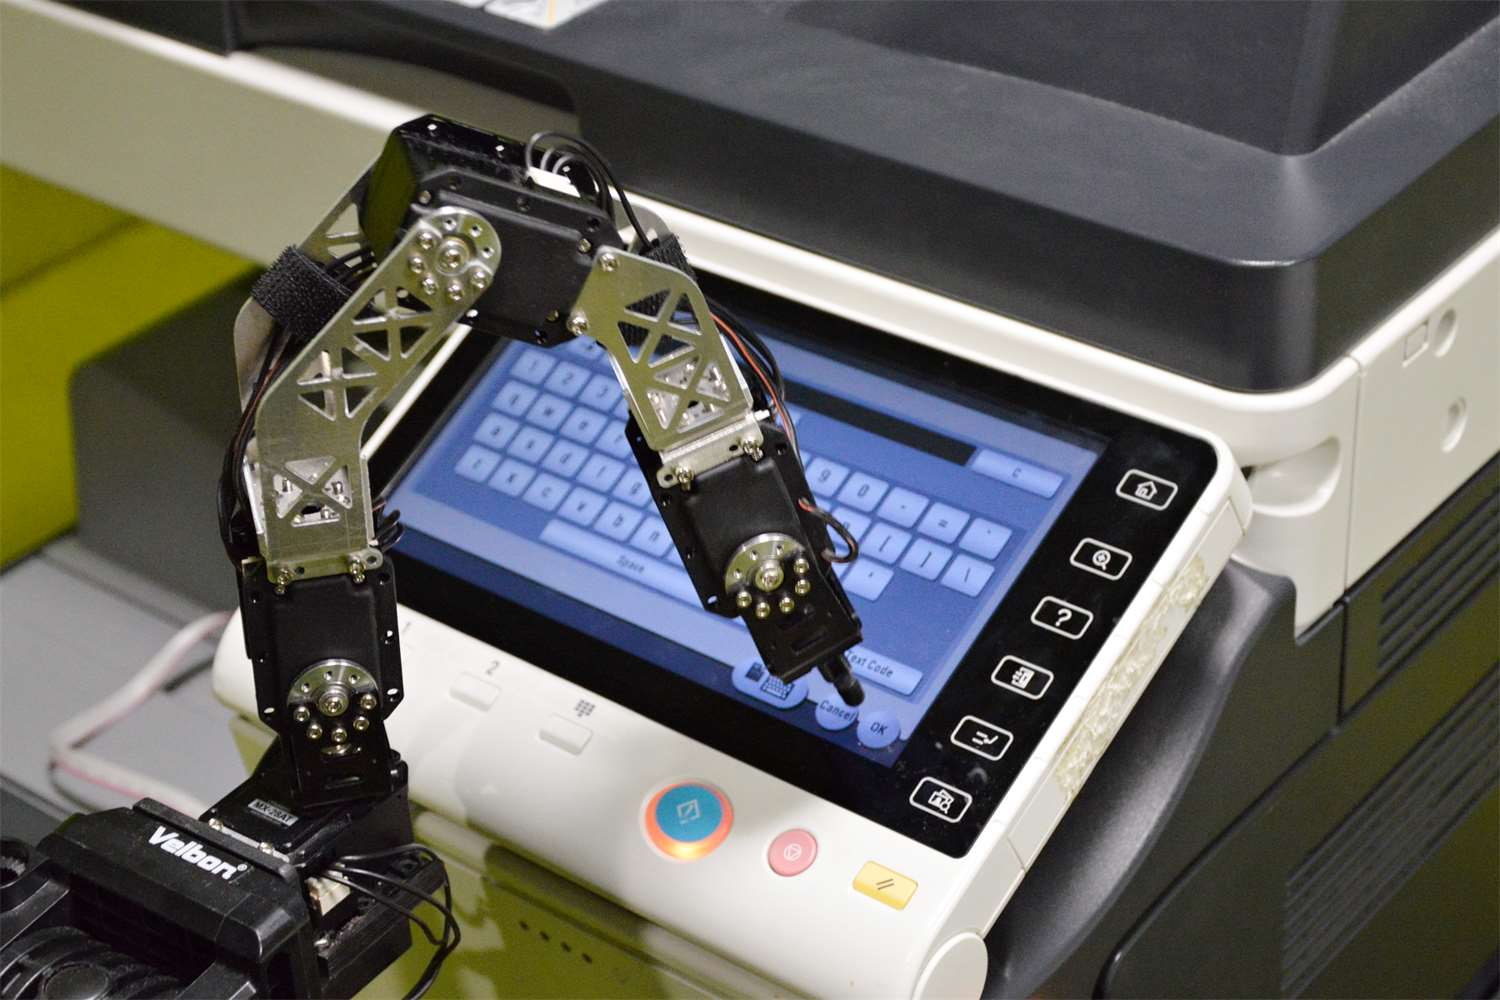
\includegraphics[width=1\textwidth]{obrazky/robot.png}
	\caption{Robot systému RQA v~průběhu testování tiskárny}
	\label{robot-img}
\end{figure}

Automatizace testování přináší mnoho výhod. Jednou z nich je ušetření nákladů, neboť testuje-li robot, není třeba platit člověka. Dále značně usnadňuje práci softwarovým vývojářům, kteří tímto způsobem šetří čas a mohou se věnovat důležitějším věcem. Roboty lze navíc nechat testovat přes noc a během dne se již jen zabývat výsledky a řešením problémů. Toto opět šetří čas a zrychluje celý proces testování. Za~následek to má rychlejší zpětnou vazbu vývojářům testovaného produktu, tedy i opravu chyb, a ve~výsledku dřívější vydání nové verze.

Mimo jiné roboti umožňují vzdálené ovládání cílového zařízení. Tato vlastnost otevírá dveře mnoha novým využitím. Vývojářům, kteří se jinak nemohou hnout od tiskáren, dává možnost pracovat z~domova či prakticky odkudkoliv. Zařízení a roboty lze spravovat lokálně a zákazníci pak mohou se~systémem pracovat na dálku odkudkoliv na světě. Stejným způsobem lze nabízet služby potenciálním zákazníkům na zkušební dobu, u~kterých instalace robota na pár týdnů nedává smysl. Vzdálené sdílení robotů navíc redukuje cenu vybavení až o~30~\% a snižuje čas potřebný pro připravení systému k~použití.

Skutečnou představu o~významu RQA pro Y~Soft lze však získat až z~čísel:
\begin{itemize}
  \item přes 1000 automatických testů,
  \item až 5x rychlejší proces testování,
  \item pokrytí testy zvýšeno o~200~\%,
  \item snížení nákladů na QA o~více než 30~\%,
  \item 98~\% vývojářů může pracovat vzdáleně,
  \item pětinásobně vyšší ROI v~porovnání s~manuálním testováním.
\end{itemize}

Nezanedbatelným přínosem RQA je i reklama firmě, neboť roboti jsou poměrně atraktivní a již existuje nejeden článek o~liduprázdných kancelářích jen s~pracujícími roboty.

\section{Architektura}
Systém je implementovaný na platformě .NET v~jazyce C\# a sestává z~několika částí. Jak je znázorněno na obrázku~\ref{rqa-architecture-img}, u~testovaného zařízení musí stát kamera, která snímá obraz a posílá ho dál ke~zpracování. Služby na backendu tento zpracovávají a komunikují s~robotem, který pak vykonává dané akce. Uživatel se~systémem interaguje pomocí webového rozhraní a samotné testy vytváří v~test frameworku. Záznamy o~událostech v~RQA jsou ukládány v~centrálním logovacím systému Graylog.

\begin{figure}[hbt]
	\centering
	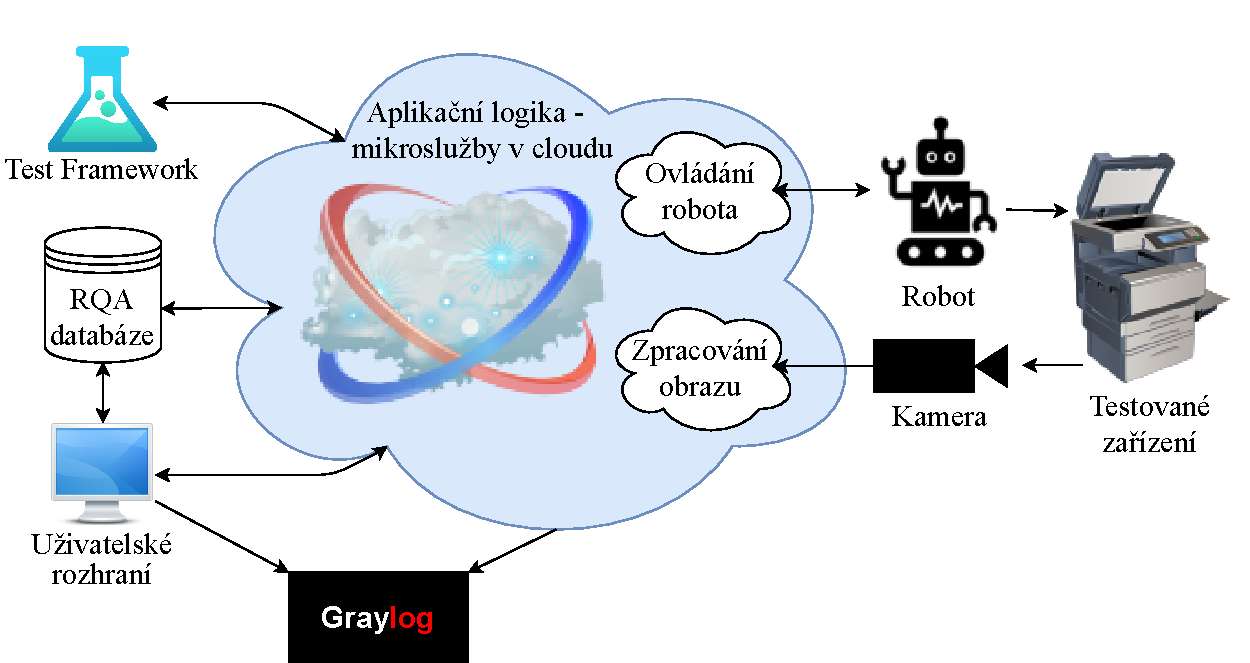
\includegraphics[width=1\textwidth]{obrazky/rqa-architecture.pdf}
	\caption{Vysokoúrovňová architektura RQA systému}
	\label{rqa-architecture-img}
\end{figure}

Pro~tuto práci jsou relevantní zejména mikroslužby aplikační logiky a systém Graylog. Vzhledem k~architektuře mikroslužeb má každou doménu (zpracování dat, počítačové vidění apod.) či subdoménu na starost zcela samostatná služba. Služby spolu komunikují prostřednictvím zpráv skrze RabitMQ. Právě tato architektura je jedním z~hlavních důvodů pro~potřebu detekce anomálií, neboť některá služba může mít problém, který ji třeba zpomaluje, aniž by si toho někdo všiml. U~monolitického systému by se tato skutečnost projevila mnohem výrazněji, neboť by ovlivnila systém jako celek. Systému Graylog je pak věnována zvláštní kapitola~\ref{graylog}.
  \chapter{Sběr a ukládání dat}
\label{sber-dat}
V~systému RQA se nachází velké množství dat různých formátů. Jedná se například o~videa a fotografie pořízená v průběhu vykonávání testů, datasety obrázků pro trénování algoritmů strojového učení, samotné záznamy o~robotech či zařízeních a mnoho dalších. Dle typu jsou tyto ukládány do~vhodných databází (objektově-relační, dokumentové...). Data, jimiž se práce zaobírá a která popisují chod systému, jsou logy. Logy se vytváří přímo v~kódu programu a ve~větších systémech se často ukládají do specializovaných logovacích systémů. V~případě RQA je tímto Graylog. První dvě sekce této kapitoly se zabývají způsobem zaznamenávání logů na platformě .NET, neboť v~ní je RQA implementováno, a systémem Graylog. Další sekce definují data udávající stav RQA systému a navrhují jejich sběr a formát pro~ukládání do~Graylogu. Následně je ukázán způsob získání dat z~Graylogu a jejich transformace do~vhodného formátu pro~algoritmy strojového učení. Na~závěr je popsána implementace představeného návrhu na platformě .NET.

\section{Zaznamenávání logů v~.NET}
Tato podkapitola vysvětluje principy logování v~.NET. Nejprve je ukázáno, jakým způsobem se logy vytvářejí. Následně je diskutováno, co lze s logy dále dělat. Na závěr jsou představeny možnosti nastavení logování.

\subsection{Vytváření logů v~.NET}
K~vytváření logů slouží objekty implementující \texttt{ILogger} rozhraní obsahující metody k~tomu určené. Pomocí nich lze specifikovat závažnost logu, jeho zprávu, výjimku v~případě chyby nebo argumenty pro~strukturované logování. Typicky se používá generická forma tohoto rozhraní \texttt{ILogger<TCategoryName>}, kde \texttt{TCategoryName} je jméno kategorie, do~které daná instance spadá a na~základě níž lze provádět filtrace nebo upřesňovat nastavení~\cite{logging}.

K~tvorbě instancí \texttt{ILogger} slouží rozhraní \texttt{ILoggerFactory} implementující návrhový vzor továrna. V~rámci tohoto rozhraní lze nastavit, jak se budou konkrétní loggery chovat. Způsob nastavení logování závisí na~tom, zda aplikace využívá tzv. obecného hostitele. Obecný hostitel je objekt, který zapouzdřuje různé zdroje aplikace, jakými jsou například právě logování, konfigurace nebo DI~\cite{generic-host}. Jestliže aplikace tohoto hostitele nepoužívá, nastavení se specifikuje v~metodě \texttt{Create()} rozhraní \texttt{ILoggerFactory}. V~opačném případě nastavení probíhá během konstrukce hostitele v~metodě \texttt{ConfigureLogging()} při~startu aplikace. Toto však nedělá nic jiného, než že \texttt{ILoggerFactory} nastaví za~programátora a vytvářené \texttt{ILogger} instance zpřístupňuje přes DI. Ve~výsledku to programátora od~explicitního používání \texttt{ILoggerFactory} zcela odstíní.

\subsection{Poskytovatelé logování}
\label{poskytovatele-logovani}
Platforma .NET podporuje API, jenž je schopno pracovat s~řadou logovacích poskytovatelů, ať už vestavěných, nebo třetích stran. Logovací poskytovatel slouží k~zobrazování či ukládání logů. Existuje jich velké množství a v~\texttt{ILoggerFactory} se nastavuje, které z~nich se budou používat. Platforma .NET nabízí několik vestavěných poskytovatelů a mnohonásobně více jich existuje od~třetích stran. Nejčastěji se jedná o~open-source projekty sloužící k~posílání logů do~konkrétních logovacích systémů. Oficiální dokumentace Microsoftu~\cite{logging} udává následující vestavěné poskytovatele: 

\begin{itemize}
  \item \emph{Console} --- Logy neukládá, pouze je zobrazuje na standardním výstupu konzole aplikace.
  \item \emph{Debug} --- Slouží k~ladění a typicky logy ukazuje jen ve~vývojovém prostředí.
  \item \emph{EventSource} --- Logy zapisuje do~zdroje událostí v závislosti na~platformě.
  \item \emph{EventLog} --- Lze použít pouze v~prostředí Windows. Logy posílá do~aplikace Windows Event Log.
\end{itemize}

K~běžně používaným externím logovacím poskytovatelům lze zařadit např. GELF nebo Serilog. Tyto zajišťují strukturované logování do vlastních logovacích systémů (Graylog a Serilog). Strukturované logování umožňuje přidávat logům dodatečné argumenty, které se pak v~logovacím systému převedou na~zvláštní pole jako na obrázku~\ref{structured-log-img}.

\begin{figure}[hbt]
	\centering
	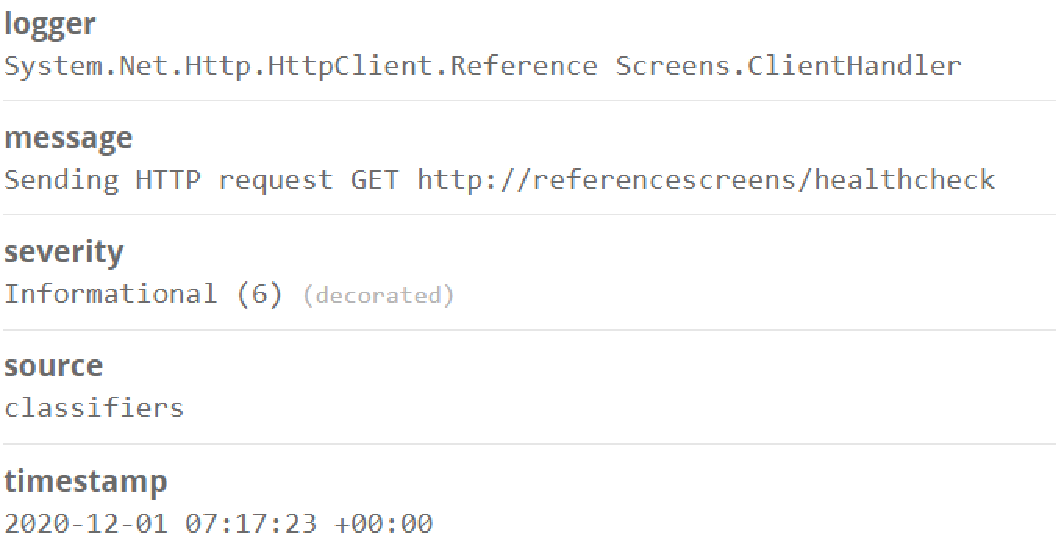
\includegraphics[width=0.85\textwidth]{obrazky/structured-log.pdf}
	\caption{Ukázka části strukturovaného logu v~systému Graylog}
	\label{structured-log-img}
\end{figure}

Pro doplňování logů o~dodatečné informace, ve~strukturovaném nebo nestrukturovaném formátu, lze využít logovací rámce. \texttt{ILogger} rozhraní obsahuje metodu \texttt{BeginScope()}, do~jejíchž parametrů lze danou informaci předat v~různém formátu v~závislosti na přetížení metody~\cite{logging, ilogger-beginscope}. Tato pak vytvoří jednorázový rámec, v~němž se ke~všem logům přidá specifikovaná informace bez nutnosti ji opakovaně udávat.

\subsection{Konfigurace logování}
Již bylo řečeno, že poskytovatelé logování se nastavují v~\texttt{ILoggerFactory}. Toto rozhraní umožňuje vytvořit i filtrovací pravidla, díky nimž lze logy zaznamenávat pouze od~určité úrovně závažnosti či jen z~vybraných kategorií~\cite{logging}. Mimo nastavení \texttt{ILoggerFactory}, které platí jen pro danou instanci~\cite{logging}, je možné logování konfigurovat i globálně. K~tomu slouží sekce \texttt{Logging} v~souboru \emph{appsettings.json}, v~němž bývají všechna potřebná nastavení .NET aplikací. Zde se nastavují parametry jednotlivých poskytovatelů, jako například adresa serveru s~logovacím systémem, port, protokol atd. Dále tu lze specifikovat výchozí úrovně závažnosti logů či filtry, ať už pro dané poskytovatele, nebo jen jejich kategorie.

\section{Graylog}
\label{graylog}
RQA používá pro~ukládání logů open-source logovací systém Graylog. Do něj se zapisuje již zmíněným GELF (Graylog Extended Log Format) poskytovatelem a už z~významu zkratky je patrné, že používá speciální formát logů pro~Graylog. V~zásadě se tento formát snaží zbavit nedostatků standardního logovacího formátu syslog, jako například omezená velikost, beztypovost nebo nemožnost komprese, a především je strukturovaný~\cite{gelf}. Pro~použití poskytovatele v~prostředí .NET je potřeba nainstalovat NuGet balík \emph{Gelf.Extensions.Logging}.

V~samotném systému Graylog lze s~logy pracovat různými způsoby. Především slouží k~vyhledání chybových zpráv v~případě, že je v~cílové aplikaci těžko dohledatelná chyba. Nabízí řadu widgetů pro~vizualizaci a práci s~logy. Umí logy předfiltrovat do~tzv. streamů, což je pouze název Graylogu pro~kategorii. Toto potom zlepšuje celkovou přehlednost nebo i rychlost vyhledávání. Významnou vlastností je také schopnost zasílat upozornění v~případě, že dojde k~nějaké události. Tato je definovaná určitou podmínkou, kterou musí příchozí log splňovat.

\section{Metriky vypovídající o stavu RQA systému}
Existuje řada metrik, jichž se používá při~monitorování systémů a aplikací. Těmito mohou být fyzické prostředky (vytížení procesoru, využití paměti RAM...), síťové parametry (propustnost, latence, ztráta paketů...) nebo aplikačně specifické metriky (návštěvnost webu...). Jelikož je žádoucí, aby RQA pracovalo efektivně a s minimálním počtem chyb, za metriky byly zvoleny délky zpracování požadavků mikroslužbami a chybovost. Následující sekce tuto volbu dále vysvětlují.

\subsection{Délka zpracování požadavku službou}
\label{delka-zpracovani-pozadavku}
Vzhledem k~architektuře mikroslužeb systém generuje nemalý síťový provoz. Většina akcí je prováděna voláním služeb, a~proto je důležité, aby délka zpracování jednotlivých požadavků byla relativně stabilní. Není tu však řeč o~času ztráveném čekáním na~odpověď klientem. Tento čas v~sobě zahrnuje i latenci, která je ovlivněna rychlostí a stabilitou sítě, k~níž je uživatel připojen. Nepřiměřená délka požadavku by tedy nemusela být zapříčiněna vadou systému, pouze pomalou lokální sítí uživatele, a anomálie by se detekovala chybně. Metrikou je míněna doba, která uplyne od~přijetí požadavku službou po~odeslání její odpovědi. Naměřený čas je tedy skutečně pouze ten, za~nějž je systém zodpovědný. Argumentovat lze případem, kdy služba volá ještě jinou službu. Latence a ostatní síťové prvky tohoto volání pak jsou v tomto čase zahrnuty. Služby však běží stále na~stejné síti, navzájem jsou pořád stejně vzdálené, a~proto tato latence bude víceméně stabilní. Rozhodně by problém zde nebyl zapříčiněn externím elementem. Případná detekce anomálie by tedy byla v~pořádku.

\subsection{Chybovost}
Chybovost lze považovat za~zřejmě nejzákladnější metriku určující stav prakticky jakéhokoliv systému i mimo obor informačních technologií. Systém by měl vykazovat minimální množství chyb, a~proto má rozhodně cenu jejich nestandardní množství detekovat. Zaznamenávat by se měly všechny možné druhy chyb během požadavku. Mezi ty patří například fatální neošetřené chyby způsobující konec provádění požadavku, ošetřené, jež provádění rozumně ukončí, nebo takové, z nichž se služba dokáže vzpamatovat.

\subsection{Nevhodné metriky}
\label{nevhodne-metriky}
Tato sekce slouží k~vysvětlení, proč některé běžně používané metriky v~oblasti monitorování aplikací a systémů nejsou použitelné pro~zadaný problém.

\subsubsection{Latence}
Latence již byla probírána v~sekci~\ref{delka-zpracovani-pozadavku}, kde se nastínilo, že je závislá na~lokální síti uživatele. Z~toho důvodu moc přesně nevypovídá o~stavu systému samotného. Dalším problémem je způsob měření. Buď by se muselo provádět externím nástrojem, nebo by každé jedno volání v~celém systému muselo být obaleno časovačem, jenž by ho měřil. První možnost by snížila soběstačnost RQA a druhá nepřipadá v úvahu, neboť by vyžadovala extrémní zásahy do~kódu a navíc se nejedná o~dobrou praktiku.

\subsubsection{Využití šířky pásma}
Využití šířky pásma (brandwidth usage) není vhodnou metrikou, neboť udává informaci o~stavu sítě, v~níž se systém nachází, nikoliv o~systému jako takovém. I~kdyby se filtroval síťový provoz generovaný jen od~RQA, je jednak nutno ho měřit externě a jednak je získaná informace zcela zbytečná. Síťová aktivita RQA totiž závisí na~tom, jestli a kolik zrovna běží testů nebo kolik uživatelů systém aktuálně používá. Tato informace je tedy variabilní a žádné systémové anomálie v~ní proto není možné hledat.

\subsubsection{Využití procesoru a operační paměti RAM}
Tyto metriky nelze měřit, neboť jsou požadavky na~služby vytvářeny asynchronně. Tím se ve~fondu vláken (\texttt{ThreadPool}) naplánuje vykonání práce a~pak již téměř nelze určit, které vlákno patří kterému požadavku~\cite{threadpool}. O~to více pak věci komplikuje kontejnerizace prvků systému a jejich nasazení v~Kubernetes. Tato platforma se navíc o~tento typ monitorování stará sama.

\section{Získání a uložení hodnot metrik}
V~této podkapitole je popsáno měření potřebných údajů a jejich zaznamenávání do~systému Graylog. Pro~tento účel se využívá koncept zvaný middleware, jenž je vysvětlen v~nadcházející sekci. Dále se rozebírá přesný způsob získání a logování informací o~požadavcích služeb a chybách. Na~závěr je ukázána organizace vytvořených logů v~Graylogu.

\subsection{Middleware v~ASP.NET}
Middleware je software, jenž se provádí před a po~zpracování každého požadavku, jako je vyobrazeno na~obrázku~\ref{middleware-img}. Požadavek či odpověď je tedy možné modifikovat. Obecně ho však lze použít pro~spuštění libovolného kódu. Metodou \texttt{Next()} se middleware opustí a pokračuje se ve~vykonávání požadavku.

\begin{figure}[hbt]
	\centering
	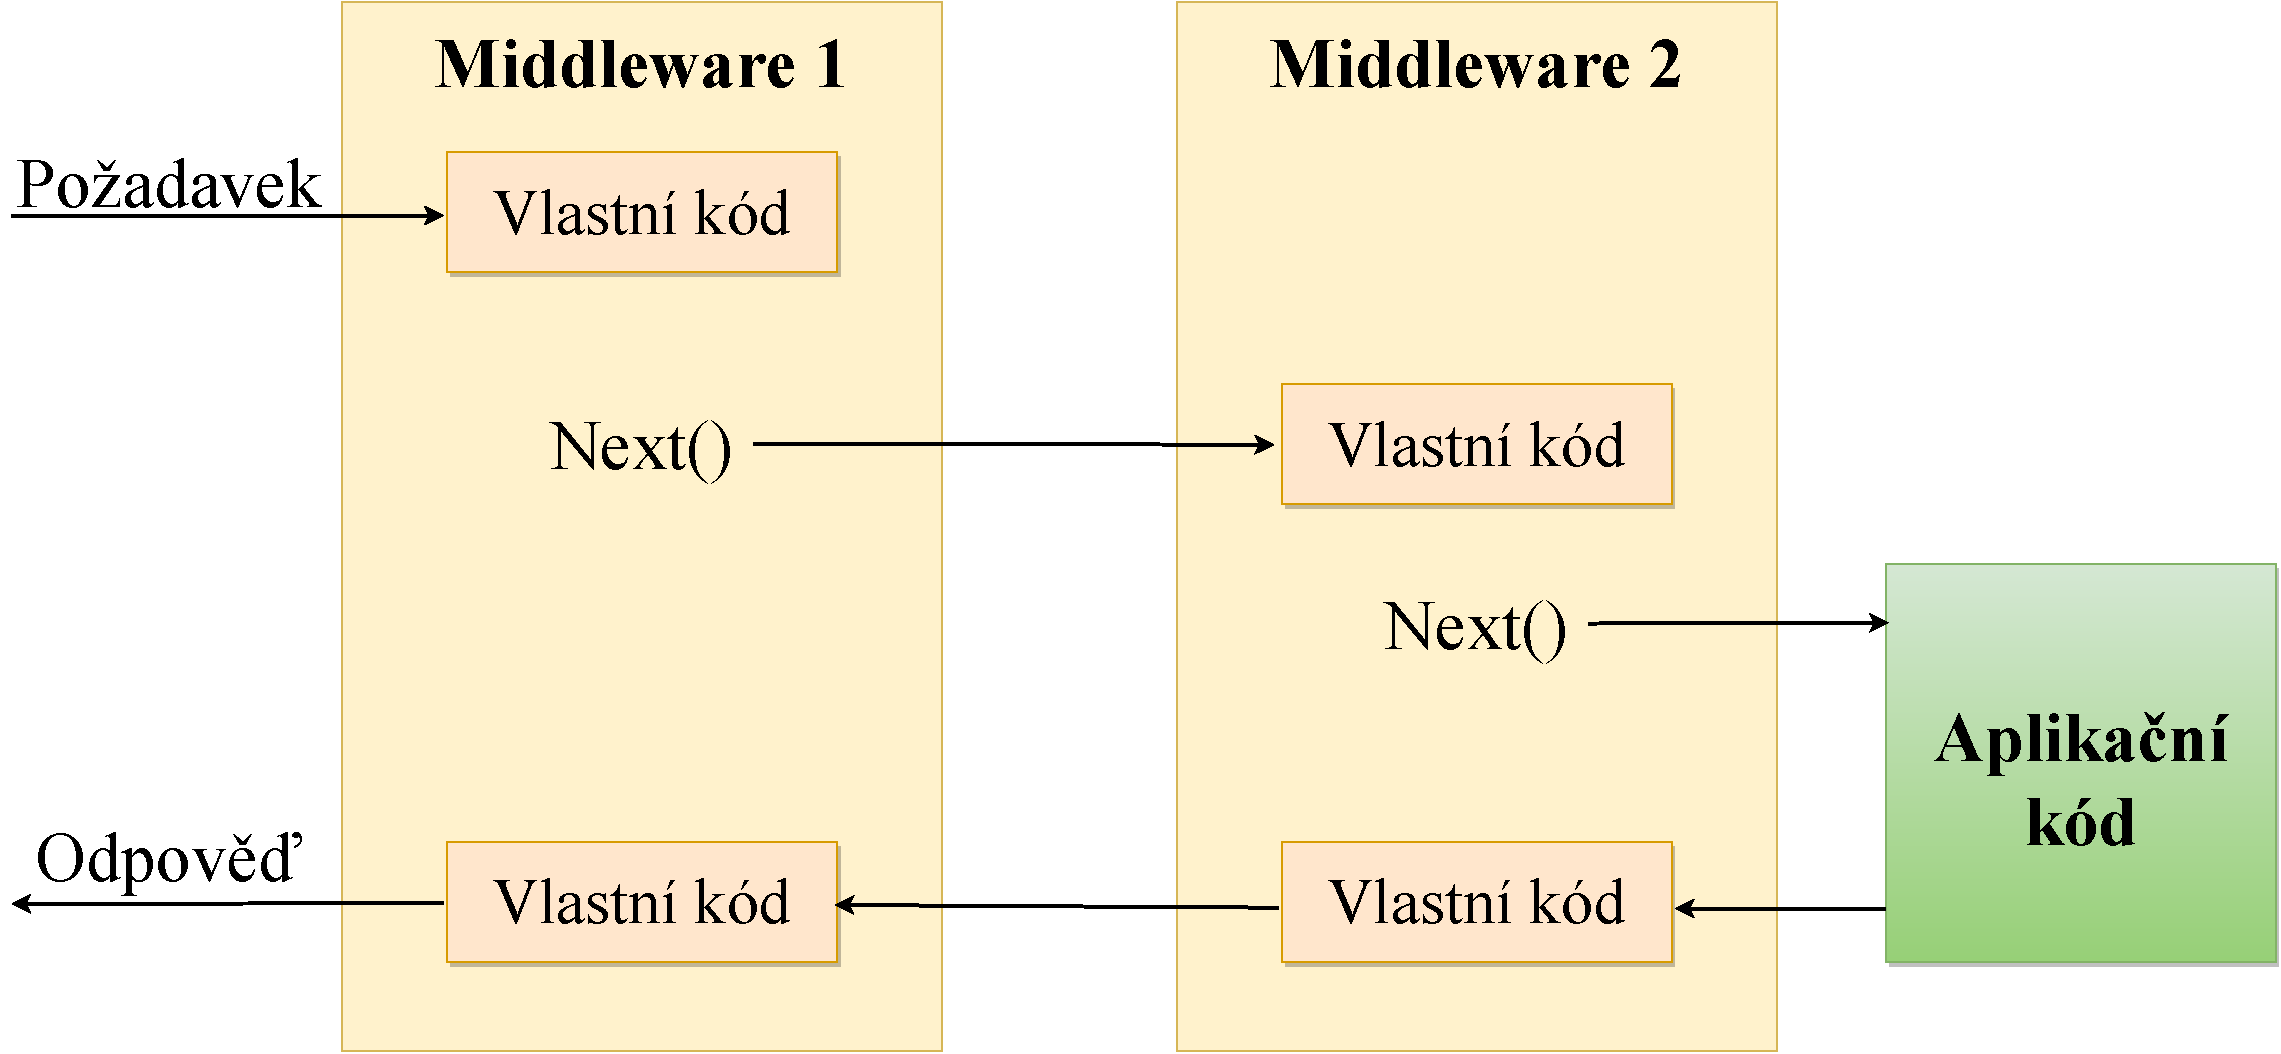
\includegraphics[width=0.9\textwidth]{obrazky/middleware.pdf}
	\caption{Princip provádění middlewaru v~ASP.NET}
	\label{middleware-img}
\end{figure}

K~plnému pochopení middlewaru je záhodno vysvětlit, jak na~platformě ASP.NET funguje zpracování webových požadavků. Klientská aplikace zašle požadavek na webový server, kde se vytvoří kanál zpracování požadavku dle konfigurace definované třídou \texttt{Startup}, v~rámci níž se mimo jiné právě middlewary registrují~\cite{middleware}. Zpracování se následně přesune do~jednotlivých middlewarů v~pořadí, v~jakém byly registrovány. Až poté teprve přijde na~řadu aplikační kód. Stejnou cestou se pak putuje zpět k~webovému serveru, který odešle odpověď. 

\subsection{Zaznamenání údajů o požadavcích na služby}
\label{zaznamenani-udaju-o-pozadavcich-na-sluzby}
Pro~vytváření logů o~délkách zpracování požadavků slouží middleware, jenž se jednotlivým mikroslužbám pouze zaregistruje. Měření probíhá tak, že se v~první fázi middlewaru spustí stopky a na~zpáteční cestě se zastaví, načež dojde k~zalogování informace.

Mimo samotnou délku požadavku je však zapotřebí mít i jiné údaje. Těmi jsou časové razítko a cíl požadavku, aby se vědělo, čeho délka se měří. Čas zaznamenání logu doplňuje ASP.NET automaticky všem logům, a~tak tento údaj není nutné řešit. Jedná se prakticky o~konec vykonávání požadavku a jeho začátek lze snadno dopočítat odečtením jeho délky. Původ logu je již taktéž znám. V~konfiguraci logování v~souboru \emph{appsettings.json} každé mikroslužby se zdroj definuje jako její název. Toto však samo o~sobě nestačí. Různé požadavky v~rámci stejné služby stále trvají odlišnou dobu, proto je třeba zaznamenat přesný cíl požadavku, kterým je dvojice kontrolér-akce. Tuto informaci pak lze vyčíst z~kontextu volání \cite{route-data}.

Logy, z~nichž se detekují anomálie v~délkách zpracování požadavků, tedy obsahují následující argumenty: časové razítko (timestamp), délka požadavku (duration), jméno služby (source), jméno kontroléru a akce (requestHandler).

\subsection{Zaznamenání údajů o chybách}
\label{zaznamenani-udaju-o-chybach}
Tato část práce řeší ten problém RQA, že aktuálně není zaznamenávání chyb v~systému jednotné. Chyby ve~službách většinou nejsou ošetřeny, neboť UI systému se o~nich nějak musí dozvědět, aby informovalo uživatele o~nezdařené akci. Z~toho důvodu nevadí nechat chybu propagovat jako klasickou interní chybu~500. Nicméně, takhle chyby kontroluje a loguje právě UI, čímž se z~pohledu logování stává zdrojem dané chyby. Zdroj je však pro~účely detekce anomálií důležitý, a~tak se logování musí dít již na~straně služby.

Implementačně nejčistším řešením je rozhraní \texttt{IExceptionFilter}. To umožňuje provádět akce nad~neošetřenými výjimkami. Dojde-li k~nějaké, provádění programu se přesune do~metody \texttt{OnException()}, v~níž lze log vytvořit. Není tedy potřeba upravovat kód v~celém systému a zanášet ho \texttt{try-catch} bloky. Problém tohoto řešení však spočívá v~tom, že pokud se vytvoří chybový log a výjimka se přepošle, aby se vypropagovala ven ze~služby, tok programu již neprojde zpětně žádným middlewarem. Nedojde tedy k~zaznamenání volání služby, jež probíhá právě v~tomto místě. Jednoduchou alternativou rozhraní \texttt{IExceptionFilter} je použití middlewaru s~metodu \texttt{Next()} vloženou do~\texttt{try} bloku. Tímto způsobem lze před přeposláním výjimky zaznamenat kromě chyby i konec požadavku. Je proto výhodné toto provádět v~middlewaru měřícím délku zpracování požadavku, neboť ten jediný má právě onu délku potřebnou pro~zaznamenání konce požadavku.

Občas je ale žádoucí chybu ošetřit a log vytvořit ručně. To by znamenalo, že by se u~každého logu musel specifikovat jeho zdroj, jímž je stejně jako u~délky zpracování požadavků dvojice kontrolér-akce. Zde přichází na~řadu metoda \texttt{BeginScope()} rozhraní \texttt{ILogger}, jež byla představena na~konci sekce~\ref{poskytovatele-logovani}. Jak to tedy provést jednoduše? Vytvoří se middleware, který pouze vytvoří logovací rámec, jenž bude logům přidávat informaci o~kontroléru a jeho akci. Vzhledem k~povaze middlewaru je tento rámec platný pro~celé volání služby. Zdroj se tedy automaticky doplní každému logu. Podmínkou tohoto přístupu je však registrace nativního routing middlewaru, tedy zavolání ASP.NET metody \texttt{UseRouting()}, před~registrací výše zmíněného. Pro~zjištění cíle požadavku je totiž zapotřebí mít již routing zprovozněn. Dále pokud se zaregistruje middleware vytvářející logovací rámec dříve než middleware, který měří délku zpracování požadavků a zachytává chyby, může se z~druhého taktéž odstranit explicitní přidávání argumentu o~kontroléru a akci. Tento předpoklad lze zajistit zpřístupněním metody, jež je zaregistruje ve~správném pořadí.

Pole chybových logů, která jsou potřebná a budou zajištěna, jsou následující: časové razítko (timestamp), jméno služby (source) a jméno kontroléru a akce (requestHandler). Chybová hláška či výjimka pro~detekci anomálií nejsou podstatné.

\subsection{Zpracování záznamů v systému Graylog}
V~podkapitole~\ref{graylog} byl vysvětlen pojem stream systému Graylog. Do~dvou takových streamů jsou logy kategorizovány. Dosahuje se tím vyšší přehlednosti, rychlosti při filtraci a tedy i stahování dat. První stream je pro~logy s~délkami zpracování požadavků. Takový log se pozná podle toho, že obsahuje všechna pole zmíněná v~sekci~\ref{zaznamenani-udaju-o-pozadavcich-na-sluzby}. Ve~druhém streamu se uchovávají chybové logy. Zda se jedná o~chybový log, se zjistí z~implicitního pole úrovně logu (\texttt{level}). Toto pole obsahuje každý log a pro~chybu je jeho hodnota~3. Z~nich se však budou brát v~potaz jen ty s~platným polem \texttt{requestHandler} kvůli webovému UI. Tam totiž mohou vznikat chyby zapříčiněné uživatelem nebo může dojít k~opětovnému zalogování chyby služby, která již byla danou službou zaznamenána, tentokrát však z~pohledu klienta, že nedostal platná data. Existence pole \texttt{requestHandler} zaručí, že k~chybě došlo v~logice webu, jeho kontroléru, a ne někde jinde.

\section{Tvorba kolekce dat ze zaznamenaných logů}
V~této fázi návrhu jsou již všechna potřebná data na~jednom místě, a sice v~Graylogu. Posledním krokem je transformovat logy na~data použitelná pro~nějaký algoritmus. Brát je přímo z~Graylogu není vhodné ze dvou důvodů. Logů ke~zpracování existují miliony, a~proto by každá detekce kvůli jejich stažení zabrala extrémně dlouho. Dále pak logy obsahují mnoho polí, která nejsou vůbec potřeba. Zjednodušení dat tedy značně sníží nároky na~paměť. V~následujících sekcích je navržen způsob stažení logů z~Graylogu, jejich transformace do~vhodného formátu a uložení na~straně aplikace detekce anomálií.

\subsection{Stažení dat pomocí Graylog REST API}
Získat data z~Graylogu bohužel není tak snadné, jak by se mohlo na~první pohled zdát. K~vyhledávání totiž využívá software Elasticsearch, jenž je limitován zobrazením pouze~10~000 položek najednou z~důvodu paměťové náročnosti~\cite{graylog-limit}. Proto nelze více než tento limit nejen zobrazit přímo v~Graylogu, ale ani stáhnout pomocí Graylog REST API, jež webové rozhraní stejně používá~\cite{graylog-api}. Limit lze sice navýšit, nicméně potom je vyžadováno výrazně více paměti a procesoru, což může zapříčinit snížení výkonnosti nebo i vznik chyb~\cite{elastic-limit}. Tento limit tedy není doporučeno měnit, a~tak nezbývá než logy stahovat po~dávkách.

Graylog REST API nabízí dvě formy vyhledávání, relativní a absolutní. U~relativního se čas specifikuje v~minutách, do~kterého se chtějí vyhledat logy od~aktuálního času. Za~normálních okolností by toto bylo preferované, avšak tím, že je nutno stahovat po~dávkách, by se s~každou dávkou posunulo časové okno. Dále by mohly nastat nepřesnosti spjaté s~latencí. Výhodnější je použít absolutní vyhledávání, které je od~pevného začátku do~pevného konce.

Chtějí-li se tedy stáhnout logy z~intervalu T\textsubscript{1} až T\textsubscript{2}, typicky od~nějakého bodu v~minulosti do~aktuálního času, vyšle se požadavek na~stažení dat z~tohoto intervalu. Stáhne-li se méně než limitních 10~000 logů, bylo staženo vše z~tohoto intervalu. Pokud však odpověď obsahuje právě tento limitní počet, nestáhlo se vše, čas T\textsubscript{1} se nastaví na~hodnotu časového razítka posledního staženého logu a vyšle se další požadavek na~stažení. Takto se stahuje po~dávkách o~10~000 záznamech, dokud se nestáhne dávka s~nižším počtem signalizující konec stahování.

\subsection{Zpracování a uložení dat}
\label{zpracovani-a-ulozeni-dat}
Vzhledem k~obrovskému množství logů, jehož stahování trvá dlouho a zdržovalo by detekci, se tyto ukládají na~straně aplikace provádějící detekci anomálií v~podobě CSV souborů. Každý typ požadavku jednotlivých služeb má svůj vlastní a to jak pro~již zanalyzovaná referenční data, tak pro~nová a doposud nezpracovaná data. Aplikace si tak udržuje všechna potřebná data a při~požadavku na~provedení detekce již nic nestahuje, pouze provede analýzu nad~doposud nezpracovanými daty. Obrázek~\ref{log-download-infrastructure-img} zobrazuje putování dat.

\begin{figure}[hbt]
	\centering
	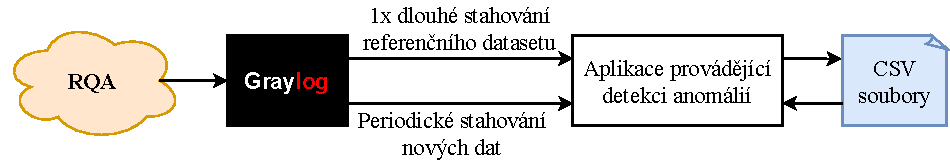
\includegraphics[width=1\textwidth]{obrazky/log-download-infrastructure.pdf}
	\caption{Komponenty podílející se na sběru dat}
	\label{log-download-infrastructure-img}
\end{figure}

Miliony referenčních logů se tedy stáhnou jen jednou a dataset se vyčistí dle postupu v~sekci~\ref{cisteni-kolekce-dat}. Nové logy se pak stahují už jen pro~krátký interval od~posledního staženého logu po~aktuální čas. Délka intervalu závisí na~frekvenci průběžného stahování. Novými logy se pak CSV soubory upravují. Úprava probíhá následovně. Nechť v~CSV souborech existují logy z~referenčního intervalu, například za~poslední týden, a nová data se stahují s~určitou periodou, třeba pět minut. Průběžně se tedy stahují logy za~cca předešlých pět minut podle posledního staženého logu a přidávají se do~souborů s~doposud nezpracovanými daty. S~požadavkem na~detekci anomálií, který je nezávislý na samotném stahování, se tyto zpracují, přidají do referenčního datasetu a naopak referenční logy starší než týden se smažou pro~zachování týdenního referenčního intervalu. Tímto způsobem se budou data neustále aktualizovat.

Před~zápisem do~CSV souborů je ještě potřeba stažené logy upravit do~vhodného formátu. Toho se docílí tím, že se pro~logy požadavků a chyb vytvoří samostatné třídy s~atributy pro~vybraná pole logů (viz~\ref{zaznamenani-udaju-o-pozadavcich-na-sluzby} a~\ref{zaznamenani-udaju-o-chybach}). Do~nich se logy z~formátu JSON deserializují a rovnou tím dojde ke zbavení se nepotřebných dat.

Princip samotného algoritmu pro~dávkové stahování a ukládání logů je popsán vývojovým diagramem v~příloze~\ref{priloha-C}. V~zásadě se nejdříve zvolí délka intervalu, z~něhož jsou logy požadovány od~aktuálního času. Poté se stáhnou všechny chybové logy. Těch nejsou miliony, takže není problém je mít prozatímně uložené v~paměti. Dále jsou stahovány dávky logů s~požadavky. Pro~jednotlivé požadavky se počítají chyby, které v~nich vznikly, a údaje se zapisují do~CSV souborů. Vzhledem k~tomu, že soubory jsou již rozděleny dle služeb a typů požadavků, zapsány jsou už jen časové razítko, délka požadavku a počet chyb jako ukazuje obrázek~\ref{csv-format-img}. Konec stahování indikuje to, že poslední dávka již není plná. V~případě stahování referenčních dat, které může trvat i hodiny, je třeba ještě zpětně stáhnout logy vzniklé během stahování. Jakmile budou data dostatečně aktuální, může se spustit samotná detekce.

\begin{figure}[hbt]
	\centering
	\begin{boxedverbatim}
Timestamp,Duration,Errors
18/01/2021 09:55:42.311 AM,37.1783,0
	\end{boxedverbatim}
	\caption{Výsledný formát dat v~CSV souboru}
	\label{csv-format-img}
\end{figure}


\section{Implementace sběru a přípravy dat}
\label{implementace-sberu-dat}
Sběr dat z~RQA do~Graylogu i stahování dat z~Graylogu je implementováno samostatnými projekty formou knihoven popsaných níže. Detekční aplikací zmíněnou v~předchozí sekci proto může být prakticky cokoliv. Konkrétní program není v~rámci řešení implementován. Pro~úplnost je však vhodné uvést všechny projekty řešení:

\begin{itemize}
  \item \emph{AnomalyDetection} --- Jedná se o~jedinou spustitelnou aplikaci řešení v~podobě webového API. Toto obsahuje pouze pár endpointů pro~stahování logů z~Graylogu a mazání stažených logů na~straně tohoto API. Ke~svému chodu využívá knihovnu \emph{AnomalyDetection.Data}, o~které bude řeč níže, žádnou vlastní logiku neimplementuje. API je snadno rozšiřitelné i pro~ovládání samotné detekce anomálií.
  \item \emph{AnomalyDetection.Application} --- Projekt implementuje detekci anomálií a je popsán v~kapitole \ref{implementace-detekce-anomalii}.
  \item \emph{AnomalyDetection.Client} --- Jednoduchý malý projekt, který slouží ke~generování klienta pro~výše zmíněné webové API pomocí nástroje NSwag.
  \item \emph{AnomalyDetection.Data} --- Obsahuje implementaci stahování dat z~Graylogu, jejich úpravy, transformace do~formátu CSV a uložení na~straně aplikace využívající tuto knihovnu.
  \item \emph{AnomalyDetection.Metrics} --- Implementuje middlewary sbírající potřebná data.
\end{itemize}

Úkolem projektu \emph{AnomalyDetection.Data} je připravit data pro~detekci anomálií. Největší podíl na~tom mají třídy \texttt{CsvHandler} a \texttt{GraylogProvider}. \texttt{CsvHandler} se stará o~veškerou práci s~CSV soubory, k čemuž využívá knihovnu \emph{CsvHelper}. Třída \texttt{GraylogProvider} pak implementuje algoritmus z~přílohy \ref{priloha-C}. Její velkou částí je vytváření dotazového url na~Graylog REST API. To vrací logy ve formátu JSON, které třída deserializuje, roztřídí podle služeb a typů požadavků a uloží pomocí \texttt{CsvHandler} do~CSV souborů tak, jak je popsáno v~sekci~\ref{zpracovani-a-ulozeni-dat}. Při~práci s~touto třídou je důležité mít na~paměti, že Graylog pracuje v~UTC čase, a~proto jsou místy nutné převody. Vlastnost \texttt{UtcHoursDiff} poskytuje rozdíl mezi lokálním a UTC časem.

V~projektu \emph{AnomalyDetection.Metrics} lze nalézt dva middlewary reflektující návrh popsaný v~sekcích~\ref{zaznamenani-udaju-o-pozadavcich-na-sluzby} a~\ref{zaznamenani-udaju-o-chybach}. Middleware \texttt{RequestDestinationMiddleware} si z~kontextu volání vytáhne název kontroléru a akce, na~něž je požadavek směřován, a vytvoří globální logovací rámec přidávající logům informaci o~cíli požadavku. Každý log vytvořený během požadavku tak bude obsahovat dodatečné pole \texttt{requestHandler} s~hodnotou \uv{\{kontrolér\}-\{akce\}}. Druhým middlewarem je \texttt{RequestDurationMiddleware}, jenž před zahájením požadavku pouze spustí stopky a na~jeho konci vytvoří log informující o~délce požadavku. Zároveň zachytává a zaznamenává všechny neošetřené chyby, neboť dělo-li by se to jinde, chyba by se propagovala tam. Vykonávání požadavku by se již nikdy nevrátilo do~tohoto middlewaru, a nezaznamenala by se proto délka onoho chybového požadavku. Projekt dále zprostředkovává metodu \texttt{UseAnomalyDetection()} pro~registraci middlewarů do~kanálu zpracování požadavku. Zahrnutí nějaké služby do~detekce anomálií je tedy natolik jednoduché, že tuto metodu pouze stačí zavolat v~metodě \texttt{Configure()} třídy \texttt{Startup} dané služby.
  \chapter{Algoritmy strojového učení pro detekci anomálií}
\label{ml-algoritmy}

Strojové učení se dělí na~dvě základní kategorie. Těmito jsou učení s~učitelem, a učení bez~učitele \cite{data-science-concepts-and-practice}. Učení s~učitelem funguje na~tom principu, že se algoritmu předají již anotovaná data~\cite{data-science-concepts-and-practice}. Dopředu je známo, kolik a jaké třídy existují a jak vypadají typická data takové třídy. Na~základě těchto dat, jimž se říká trénovací, dokáže algoritmus vytvořit model schopný rozřazovat nově příchozí neznámá data do~daných tříd~\cite{data-science-concepts-and-practice}. Pro~detekci anomálií to lze použít v~případech, kdy se dobře ví, jaké anomálie mohou nastat a jak tyto vypadají. Poté se již jen neznámá data předají modelu, jenž se rozhodne, zda se jedná o~anomálii či nikoliv.

U~učení bez~učitele se ztrácí komfort označených dat. Algoritmy dopředu neví, jaké třídy existují, a typicky je jejich úkolem data na~základě jistého druhu podobnosti do~nějakých tříd rozdělit~\cite{data-science-concepts-and-practice}. Za~tímto účelem algoritmy vyžadují určité parametry, dle kterých rozdělovat. Častým je například právě počet tříd, do~nichž data rozdělit. Vzhledem k~dopředné neznalosti dat tu většinou nedochází k~trénování nějakého modelu, nýbrž výpočet probíhá nad všemi vstupními daty~\cite{supervised-vs-unsupervised-learning}. Anomálie se poté detekují tím způsobem, že z~nalezených tříd některá právě anomální data vyčnívají, nebo se do~žádné třídy ani nepřiřadí.

K~detekci anomálií se typicky používá učení bez učitele~\cite{intro-to-anomaly-detection}, jímž se také práce zabývá, a to z následujících důvodů. Vzhledem k~tomu, že anomálie se dějí velmi zřídka, neboť pokud by byly pravidelné, již by se jednalo o~standardní chování, tak je velmi těžké nasbírat trénovací data~\cite{intro-to-anomaly-detection}. V~mnoha případech užití, mezi kterými je i například právě monitorování systémů, by se modely musely s~příchodem nových dat v~čase neustále přetrénovávat, což je nepraktické. Učení bez učitele tyto problémy řešit nemusí. Pokud se navíc objeví zcela nový typ anomálie, algoritmy učení s~učitelem anomálii nedokáží rozpoznat, neboť taková data při~trénování neviděly~\cite{intro-to-anomaly-detection}. Algoritmus učení bez učitele tuto detekovat dokáže, protože vidí pouze vybočující data od~standardu a nesnaží se je nijak kategorizovat do~třídy \uv{anomálie}.

Pro~shrnutí, jestliže se předem ví, co přesně detekovat a jak to vypadá, je vhodné použít učení s~učitelem. Natrénuje se model, který bude poměrně rychle určovat, zda je jeho vstup anomální, či nikoliv. Pokud však dopředu nejsou anomálie zcela známé, mohou se měnit v~čase, nelze je kategorizovat, je zapotřebí učení bez učitele.

V~případě RQA je jedinou cestou učení bez~učitele, neboť o~datech neexistuje žádná dopředná znalost. Trénovací dataset by pro~učení s~učitelem šlo vytvořit pouze manuálním průchodem a vyčleněním anomálií z milionů logů nebo vhodným použitím právě učení bez~učitele. Neustálý příchod nových dat by znamenal nutnost pravidelného přetrénování. Natrénovaný model by navíc musel tisíce nově příchozích logů zpracovávat samostatně, zatímco algoritmus učení bez učitele to provede v~jediném výpočtu. Nadcházející sekce se zabývají různými typy algoritmů učení bez učitele, jejich zástupci a způsobem využití pro~detekci anomálií.

\section{Shluková analýza}
Shluková analýza slouží k~rozdělení neznámých dat do~shluků. Prvky těchto shluků, nebo také tříd, si pak jsou v~určitých aspektech podobné. Anomálie lze rozpoznat podle topologie shluků nebo tím, že některý prvek žádnému shluku ani nebyl přiřazen.

\subsection{Kategorizace algoritmů}
Existuje několik způsobů členění shlukových algoritmů. To znamená, že jeden algoritmus může spadat do~více skupin. V~následujících sekcích jsou uvedeny nejběžnější kategorie.

\subsubsection{Rozdělovací algoritmy}
V~anglické terminologii jsou jinak označovány jako \uv{centroid-based} algoritmy~\cite{cluster-methods-article}. Jedná se o~algoritmy, které data rozdělí do~předem stanoveného počtu tříd. Na~začátku se pro~každou třídu určí její centrální bod, ke~kterému se poté ostatní body přidružují na~základě třeba vzdálenosti či jiných parametrů~\cite{cluster-methods-article}. Do~této kategorie spadají například K-Means, SOM nebo jistým způsobem i GMM. Tyto algoritmy přiřadí všechny prvky nějakému shluku. Z~toho důvodu nejsou schopny odhalit jednotlivé outliery, nicméně dokáží rozpoznat celý anomální shluk.

\subsubsection{Hierarchické algoritmy}
Na rozdíl od~rozdělovacích algoritmů, které rovnou počítají se všemi daty, pracují hierarchické algoritmy tak, že shlukování provádí nad~podmnožinami datasetu~\cite{cluster-methods-article}. Tím se získají částečné shluky, které lze dále spojovat do~větších například aglomerativními metodami (single/complete linkage) \cite{cluster-methods-article}. Vznikne tak hierarchický strom shluků, nebo-li dendrogram~\cite{cluster-methods-book, cluster-methods-article}.
Typickým představitelem je kupříkladu HDBSCAN.

\subsubsection{Algoritmy založené na~hustotě}
U~těchto algoritmů se shluky vytvářejí na~základě hustoty bodů v~prostoru. Jejich velkou výhodou je to, že dopředu není nutno znát počet tříd, do~kterých se data rozdělují~\cite{cluster-methods-book}. Dokonce nemusí dostatečně odlehlá data přiřadit žádné třídě~\cite{cluster-methods-book}. To znamená, že jsou schopny relativně snadno detekovat šum. K~těmto metodám se řadí DBSCAN, HDBSCAN nebo OPTICS.

\subsubsection{Algoritmy založené na~pravděpodobnostním rozložení}
Tyto algoritmy jsou také občas označované jako \uv{algoritmy založené na~modelech}, kde se modelem typicky myslí pravděpodobnostní rozložení~\cite{cluster-methods-book}. Shluky jsou zde definované jako objekty patřící do~stejného rozložení~\cite{cluster-methods-book}. Nejčastěji používaným rozložením je Gaussovo a algoritmem proto GMM.

\subsection{K-Means}
Jedná se o rozdělovací algoritmus shlukující všechna data do~předem stanoveného počtu tříd. Kniha \emph{Data Science: Concepts and Practise}~\cite{data-science-concepts-and-practice} popisuje algoritmus následovně:

\begin{enumerate}
    \item Z~dat se náhodně vybere tolik bodů, kolik je tříd, a ty slouží jako centrální body.
    \item Vypočítají se vzdálenosti všech bodů od~každého centrálního bodu a přiřadí se k~tomu s~nejmenší vzdáleností.
    \item Spočítá se střed každého shluku, který se stává jeho novým centrálním bodem.
    \item Pokud žádný bod nezměnil třídu, algoritmus končí, jinak se opakuje od~bodu 2.
\end{enumerate}

Dále lze v knize najít několik běžně používaných typů vzdáleností. Nejrozšířenější je Eukleidovská vzdálenost, nebo-li délka úsečky mezi dvěma body. Další je Manhattanská vzdálenost, která měří cestu k~cíli pouze po~pravoúhlých cestách a jež si své jméno vydobyla podle cestování po~New Yorku. Chebyshevova vzdálenost zase udává maximální rozdíl mezi všemi atributy datasetu. V~případě obrázku~\ref{k-means-img}(b) je to maximum z [(3 - 1), (1 - 2)] = 2. 

\begin{figure}[tbh]
    \centering
    \subfloat[\centering Shlukování dat algoritmem K-Means]{{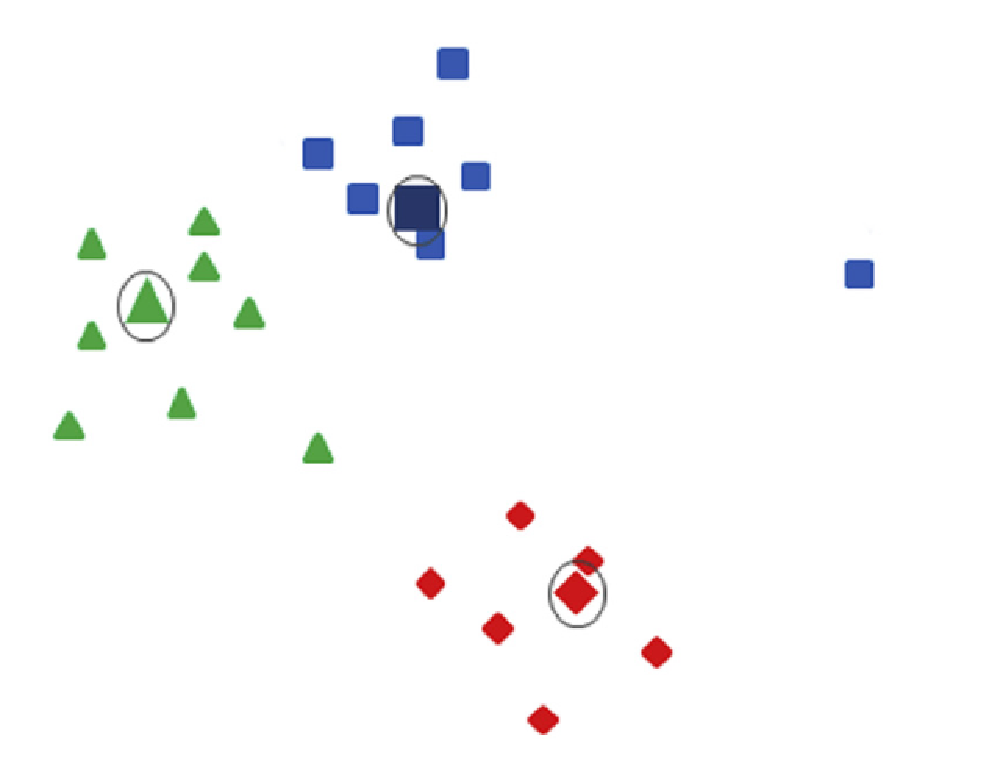
\includegraphics[width=7cm]{obrazky/k-means.pdf} }}
    \qquad
    \subfloat[\centering Typy vzdáleností používané v~K-Means]{{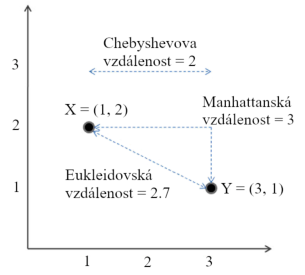
\includegraphics[width=7cm]{obrazky/distances.pdf} }}
    \caption{Výsledek algoritmu K-Means a různé typy vzdáleností (upraveno z \cite{data-science-concepts-and-practice})}
    \label{k-means-img}
\end{figure}

\subsection{GMM}
GMM (Gaussian Mixture Model), nebo-li směs Gaussových rozložení, je jeden z~nejvýznamnějších algoritmů strojového učení. Mimo shlukování ho lze využít i pro~klasifikaci. Jako se u~K-Means na počátku zvolí centrální body, tak tu se vytvoří určitý počet normálních rozložení. Body se poté jednotlivým rozložením přiřazují (viz. obr.~\ref{gmm-img}) a po~dokončení jednoho cyklu se přepočítají jejich parametry, tedy střed a kovarianční matice~\cite{sur-gmm-lecture}. Tímto způsobem se model trénuje, čili hledají se optimální parametry Gaussových rozložení~\cite{sur-gmm-lecture}. Počet cyklů nelze určit deterministicky, nýbrž se experimentálně hledá nejlepší řešení. Z~toho je patrné, že GMM trpí vadou možného přetrénování. Dále lze u~GMM zvolit specifický trénovací algoritmus, z~nichž dva jsou nejznámější. Výsledkem Viterbiho trénování jsou data, která jsou jednoznačně přiřazena (tvrdé přiřazení) určitým rozložením~\cite{sur-gmm-lecture}. Expectation Maximization (EM) naopak data přiřazuje měkce pomocí vah, kterými jsou posteriorní pravděpodobnosti spočítané aktuálním modelem~\cite{sur-gmm-lecture}. Nové parametry rozložení se poté při~trénování počítají váhovanými průměry, namísto prostých~\cite{sur-gmm-lecture}. Z~toho důvodu je EM algoritmus přesnější.

\begin{figure}[hbt]
	\centering
	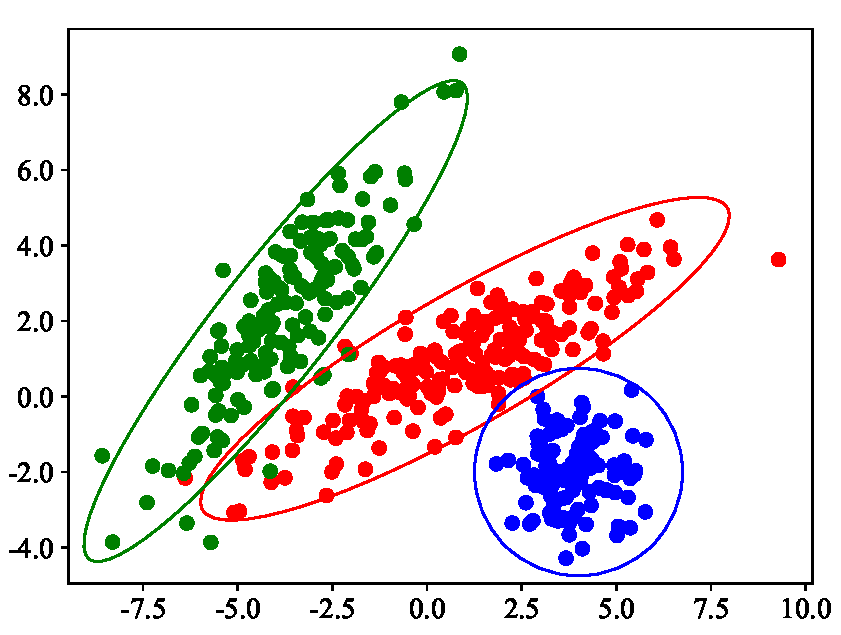
\includegraphics[width=0.7\textwidth]{obrazky/gmm.pdf}
	\caption{Rozdělení dat do~3~shluků algoritmem GMM}
	\label{gmm-img}
\end{figure}

\subsection{SOM}
Algoritmus SOM (Self-Organizing-Maps), nebo také Kohonenova mapa podle jeho tvůrce, je speciální typ neuronové sítě. Produkuje nízkodimenzionální diskretizovanou reprezentaci vstupních dat v~podobě mapy~\cite{som-web}. Od~jiných neuronových sítí se liší především tím, že se neučí na~základě opravy chyb, jako je tomu například u~gradientního sestupu, nýbrž určité sousední funkce, která zachovává zvolenou topologii mapy~\cite{som-web}. Topologie mapy neuronů se určuje na začátku algoritmu a typicky se volí obdélníková nebo hexagonální \cite{data-science-concepts-and-practice}. Jednotlivé neurony zde prakticky specifikují shluky. Práce \emph{Brief Review of~Self-Organizing Maps} \cite{som-article} algoritmus popisuje následovně:

\begin{enumerate}
    \item Náhodně se inicializují váhy neuronů každému vstupnímu bodu (viz. w\textsubscript{ij} na~obr.~\ref{som-img}).
    \item Náhodně se vybere jeden ze vstupních vektorů.
    \item Zvolí se vítězný neuron nejčastěji na~základě eukleidovské vzdálenosti od~prvků vybraného vstupního vektoru.
    \item Upraví se váhy neuronů zmíněnou sousední funkcí.
    \item Opakuje se od~bodu 2, dokud neskončí trénování.
\end{enumerate}

Úprava vah a sousední funkce zde nejsou rozebírány, neboť by si vzhledem k~jejich různým typům a složitosti zasloužily samostatnou kapitolu. Podstatné však je, že kromě váhy vítězného neuronu budou vylepšeny i váhy sousedních neuronů v~závislosti na~jejich vzdálenostech od~vítěze.

\begin{figure}[hbt]
	\centering
	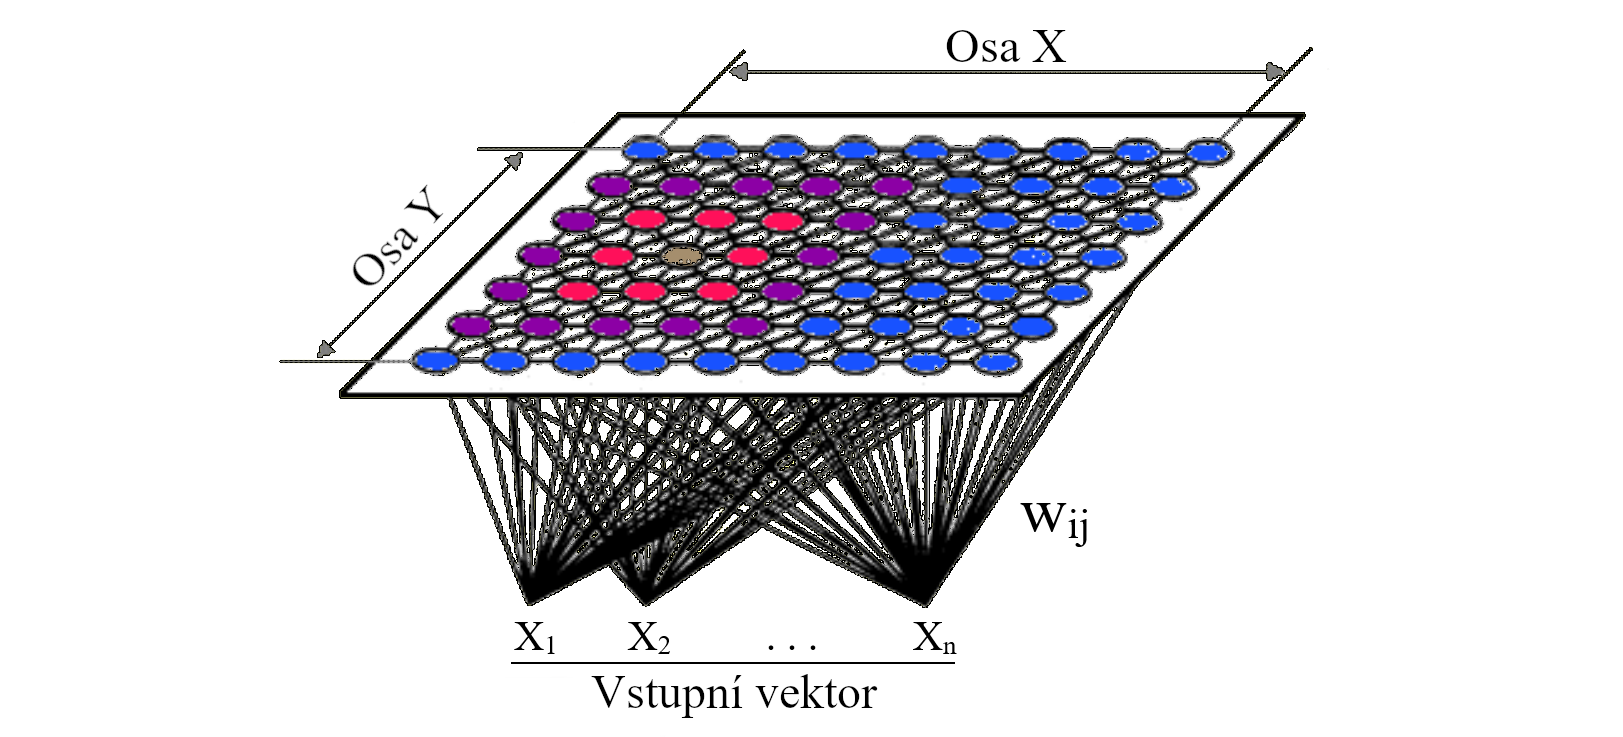
\includegraphics[width=0.85\textwidth]{obrazky/som.png}
	\caption{Ukázka propojení vstupů s~neurony a jejich váhami v~SOM (upraveno z~\cite{som-web})}
	\label{som-img}
\end{figure}

\subsection{DBSCAN}
Zkratka tohoto algoritmu znamená Density based spatial clustering of applications with noise, nebo-li prostorové shlukování aplikací s~šumem na~základě hustoty. DBSCAN je velmi rychlý algoritmus a jeho přednostmi jsou, že snadno odhalí šum a není třeba dopředu znát počet shluků. Tato informace totiž velmi často není známá. Jediné, co je třeba určit, je v~podstatě definice hustoty. Typicky se hustota měří v~kruhovém prostoru kolem bodů, a~proto je zapotřebí zvolit jisté \textepsilon, což není nic jiného, než poloměr onoho kruhu \cite{data-science-concepts-and-practice}. Druhým parametrem je minimální počet bodů, od~kterého se prostor považuje za~hustý \cite{data-science-concepts-and-practice}. Tento parametr bude dále v~práci značen jako MinPts z~anglického \uv{minimum points}. Pro každý bod se poté určí, zda leží v~husté oblasti, nebo ne. Dle literatury \cite{data-science-concepts-and-practice} se body dělí na 3 typy: 

\begin{itemize}
  \item \emph{Jádrové body} --- Mají dostatečný počet sousedů, jsou proto v~husté oblasti.
  \item \emph{Krajní body} --- Nemají dostatek sousedů, nicméně stále leží v~dosahu \textepsilon\space některého z~jádrových bodů, a~proto jsou ještě členy shluku.
  \item \emph{Šum} --- Nemá dostatek sousedů ani neleží v~dosahu \textepsilon\space některého z~jádrových bodů. Není přiřazen žádnému shluku.
\end{itemize}

Jak lze vidět na~obrázku~\ref{dbscan-vs-k-means-img}, shlukování na~základě hustoty lépe seskupí body tvořící útvary než jiné algoritmy. Nevýhodou algoritmu je však to, že nedokáže rozpoznat shluky různých hustot \cite{data-science-concepts-and-practice}. De~facto data rozděluje pouze na husté a řídké.

\begin{figure}[hbt]
	\centering
	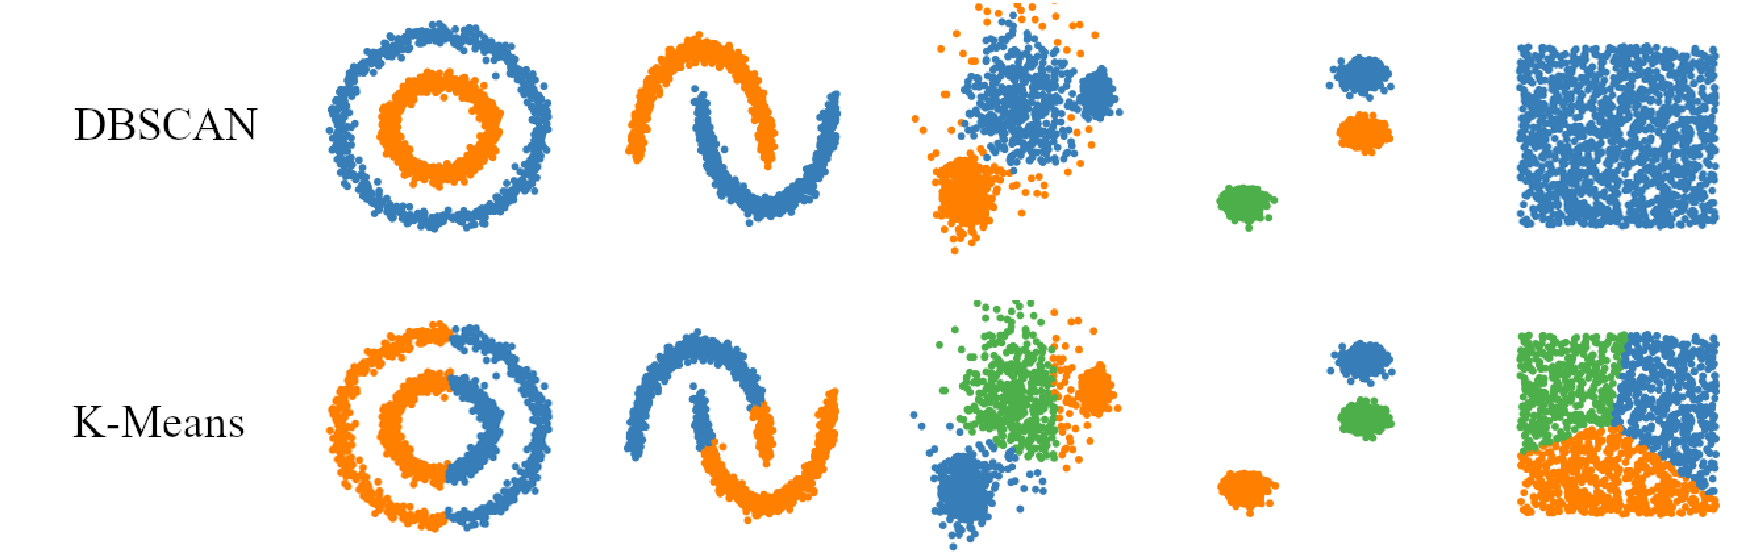
\includegraphics[width=0.83\textwidth]{obrazky/dbscan-vs-k-means.pdf}
	\caption{Porovnání shlukování algoritmy DBSCAN a K-Means (upraveno z~\cite{dbscan-vs-k-means})}
	\label{dbscan-vs-k-means-img}
\end{figure}

\subsection{HDBSCAN}
HDBSCAN (hierarchický DBSCAN) je rozšíření DBSCAN algoritmu používající hierarchické shlukování. Algoritmus je poměrně komplexní a skládá se z~mnoha kroků. Nejprve je potřeba zvolit metriku vzdálenosti mezi body. Nelze tu použít klasickou eukleidovskou vzdálenost, neboť není cílem shlukovat body, jež jsou si pouze eukleidovsky blízké, nýbrž musí být zároveň i husté~\cite{hdbscan-video}. K~tomu slouží tzv. vzdálenost vzájemné dosažitelnosti (mutual reachability distance MRD), kterou lze spočítat pomocí vzorce~\ref{mrd-rovnice}~\cite{hdbscan}:

\begin{equation}
\label{mrd-rovnice}
d_{mrd}(a,b) = max\{\epsilon_a, \epsilon_b, d(a,b)\}
\end{equation}

Hodnoty \emph{a,b} jsou dané body, \textepsilon\space je poloměr oblasti jako u~DBSCANu. Není však nastaven ad~hoc, nýbrž se jedná o~vzdálenost ke~\emph{k}-tému sousedu. Funkce \emph{d()} je klasická eukleidovská vzdálenost dvou bodů.

Pro vytvoření hierarchického dendrogramu nechť je dán graf, jehož vrcholy jsou jednotlivé body a hrany mají váhy rovny vzdálenostem mezi nimi. Zvolí se práh s vysokou hodnotou, jež se bude v~dalších průchodech postupně snižovat~\cite{hdbscan}. Během průchodů se odstraňují hrany s~váhou vyšší než je aktuální prahová hodnota, čímž se graf začne rozpojovat do~propojených komponent a tím vznikat hierarchický strom~\cite{hdbscan}. Vzhledem k~tomu, že existuje \emph{n\textsuperscript{2}} hran, měl by algoritmus asymptotickou složitost \emph{O(n\textsuperscript{2})}, a~proto je graf pro~zrychlení dopředu zredukován na~minimální kostru (obr.~\ref{hdbscan-dendrogram-img}a) Jarníkovým (Primovým) nebo Borůvkovým algoritmem~\cite{hdbscan}. Výsledný dendrogram (obr.~\ref{hdbscan-dendrogram-img}b) poté vznikne spojováním hran, dokud se nedojde ke kořenu.

\begin{figure}[hbt]
    \centering
    \subfloat[\centering Minimální kostra grafu]{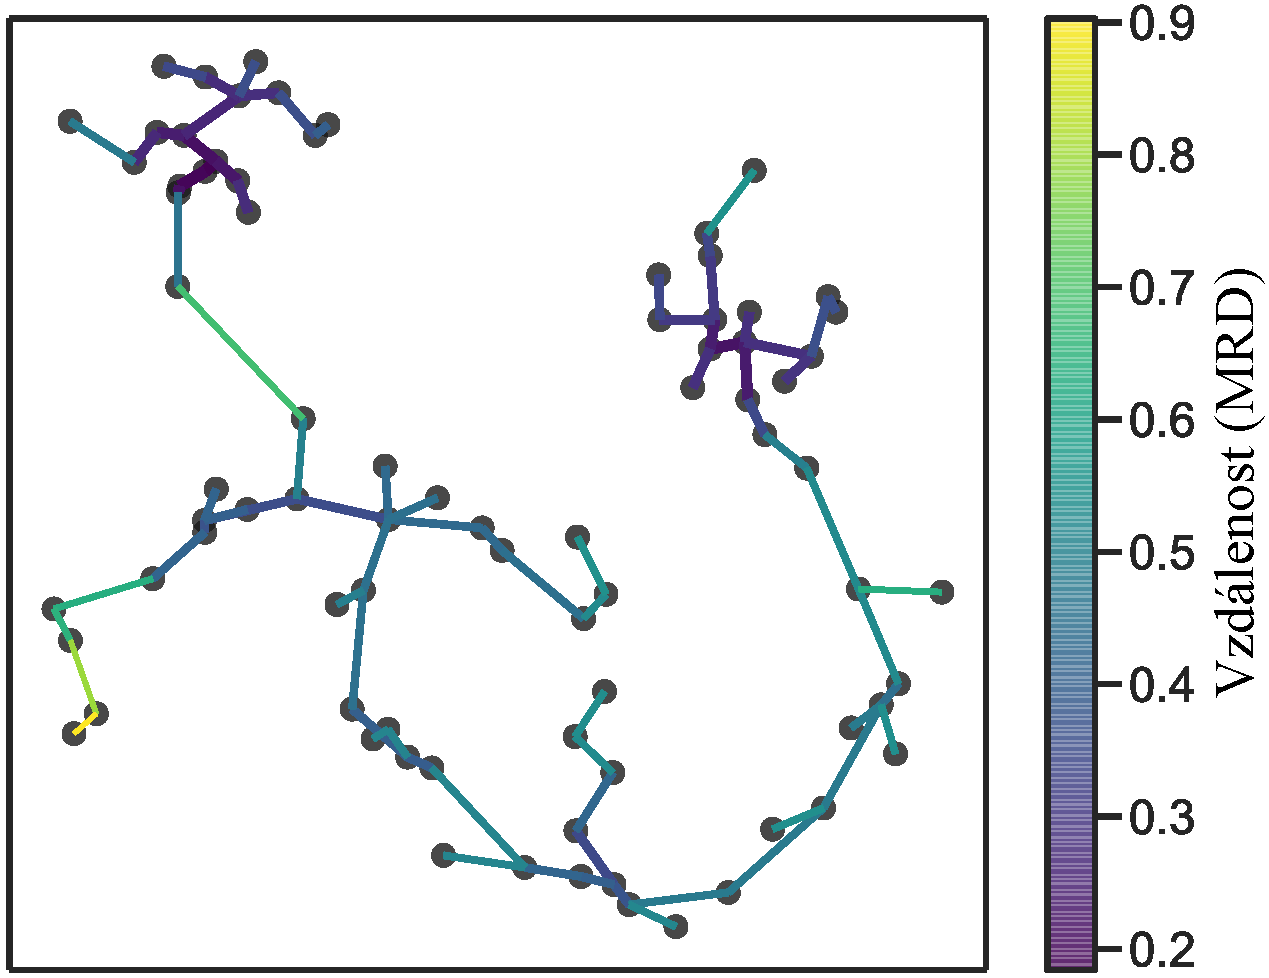
\includegraphics[width=6.9cm]{obrazky/hdbscan-tree.pdf} }
    \subfloat[\centering Výsledný dendrogram]{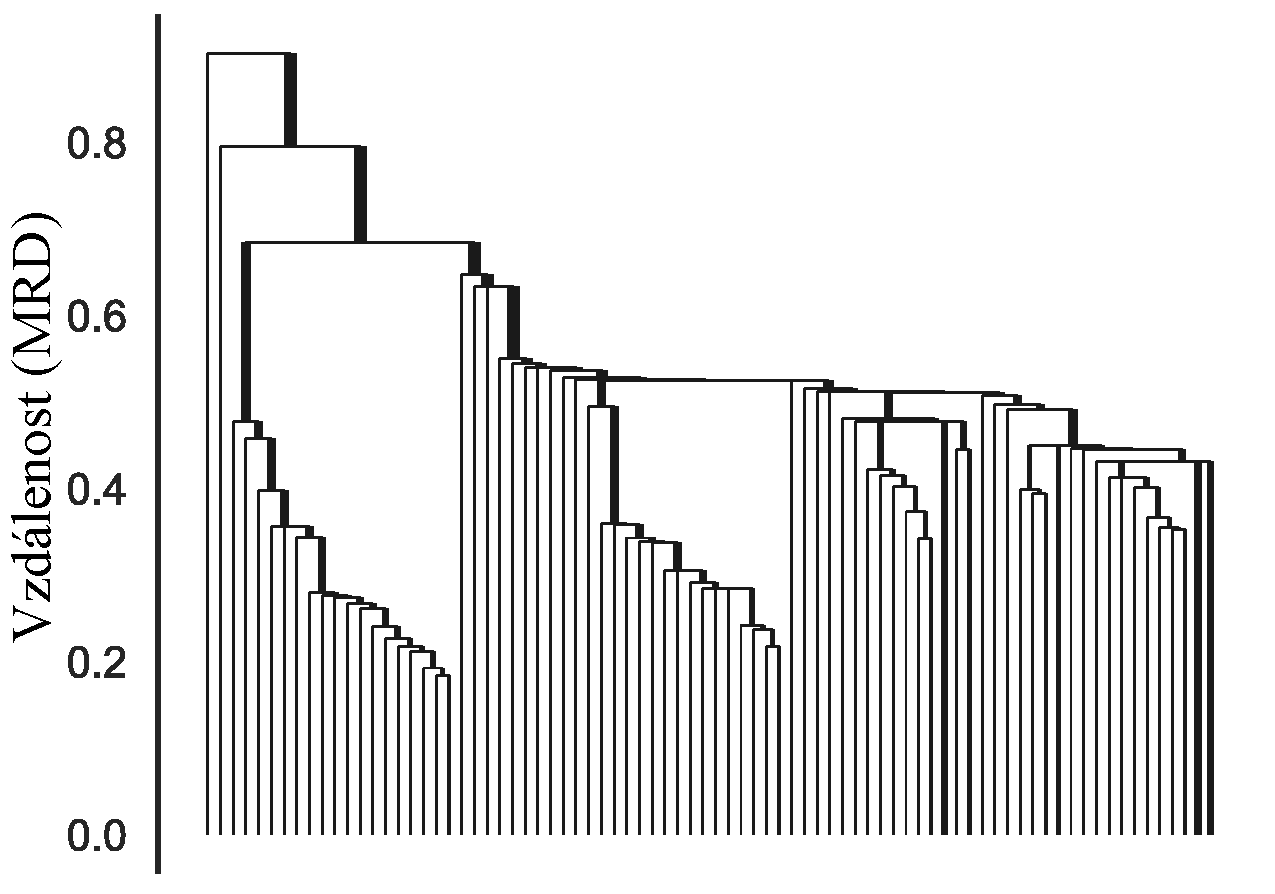
\includegraphics[width=7.7cm]{obrazky/hdbscan-dendrogram.pdf} }
    \caption{Vytvořený dendrogram s~využitím minimální kostry algoritmem HDBSCAN}
    \label{hdbscan-dendrogram-img}
\end{figure}

V~tomto bodě jsou již známy shluky, nicméně v~praxi není žádoucí reprezentace hierarchickou strukturou, nýbrž sadou daných shluků. DBSCAN by zde vytyčil práh minimálních bodů pro hustou oblast, dendrogram tímto prahem prořízl, shluky pod čarou zahodil jako šum, zbytek si ponechal a skončil~\cite{hdbscan}.
HDBSCAN však napravuje nedostatek DBSCANU ve variabilitě hustot a dendrogram prořízne v~různých místech. Jak se to provede? Dopředu se určí minimální velikost shluku a při~dělení shluku se s~touto porovná velikost obou potomků~\cite{hdbscan}. Pokud jsou oba větší, dělení je platné a ve~stromu vzniknou nové větve~\cite{hdbscan}. V~opačném případě se potomci zahodí jako šum~\cite{hdbscan}. Tím vznikne kondenzovaný strom~\ref{hdbscan-result-img}.

Nyní již zbývá pouze zvolit výsledné shluky. Prvním pravidlem je, že pokud se již některý vybere, nesmí se použít žádný z~jeho potomků~\cite{hdbscan}. Volba shluků se provádí na~základě jejich stability, jejímuž výpočtu~\ref{stabilita-rovnice} slouží zvláštní proměnná \(\lambda = 1 / d_{mrd}\), kde vzdálenost \emph{d\textsubscript{mrd}} je hodnota osy y v~dendrogramu~\ref{hdbscan-dendrogram-img}(b)~\cite{hdbscan}.

\begin{equation}
\label{stabilita-rovnice}
S = \sum_{i\in shluk}(\lambda_i - \lambda_{v})
\end{equation}

\textlambda\textsubscript{i} je zde lambda jednotlivých bodů shluku a \textlambda\textsubscript{v} pak lambda vzniku shluku. Následně se jako vybrané shluky zvolí listy stromu a postupuje se ke~kořenu. Spočítá se stabilita vybraných shluků a jejich rodičů. Pokud je stabilita rodiče větší než suma stabilit potomků S\textsubscript{p}, rodič se stává novým zvoleným prvkem~\cite{hdbscan}. V~opačném případě se rodiči nastaví hodnota stability na~S\textsubscript{p}~\cite{hdbscan}.

\begin{figure}[hbt]
	\centering
	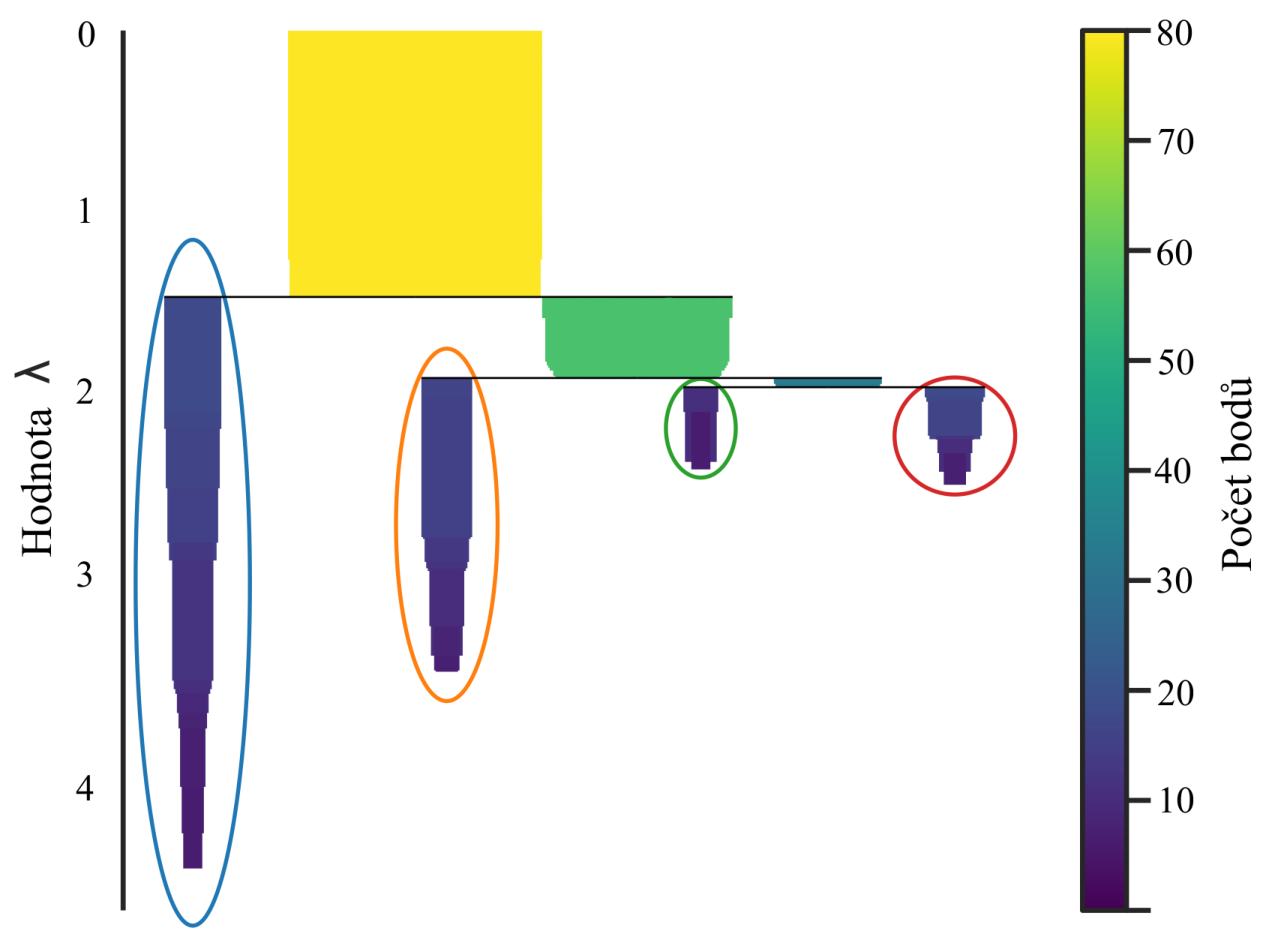
\includegraphics[width=0.7\textwidth]{obrazky/hdbscan-condensed-tree.pdf}
	\caption{Kondenzovaný strom s vyznačenými výslednými shluky}
	\label{hdbscan-result-img}
\end{figure}

Výsledkem HDBSCANu jsou shluky podobné těm od~DBSCANu na obrázku~\ref{dbscan-vs-k-means-img} s~tím rozdílem, že dokáže pojmout více stupňů hustot. Navíc vzhledem ke~znalosti hodnoty \textlambda\textsubscript{i} je schopen vytvořit měkké skóre určující, jak moc bod k~danému shluku patří~\cite{hdbscan}. Při~zanedbání určitých konstant lze jeho časovou složitost vnímat jako \emph{O(NlogN)}~\cite{hdbscan-video}, což ho řadí mezi nejrychlejší shlukovací algoritmy k~dispozici.

\subsection{OPTICS}
K~algoritmům založených na~hustotě patří také OPTICS (Ordering Points to Identify Cluster Structure). Jedná se o~příbuzný algoritmus DBSCANu, jenž řeší problém variability hustoty a zjednodušuje nalezení počátečních parametrů definující jádrové body. Kromě jádrové vzdálenosti \textepsilon\space pracuje ještě s~tzv. dosažitelnou vzdáleností (reachability distance RD)~\cite{optics}, která je zjednodušením MRD u~HDBSCANu. Jedná se o~vzdálenost mezi jádrovým bodem \emph{p} a nějakým jiným bodem \emph{q}~\cite{optics}. Platí pro~ni vztah~\ref{rd-rovnice}~\cite{optics}:

\begin{equation}
\label{rd-rovnice}
d_{rd}(p,q) = max\{\epsilon_p, d(p,q)\}
\end{equation}

V~rovnici je opět \textepsilon\textsubscript{p}\space poloměrem oblasti \emph{p} jako u~DBSCANu a funkce d() eukleidovskou vzdáleností.

Algoritmus spočívá v~tom, že se vypočítají dosažitelné vzdálenosti a data se poté seřadí tak, aby spolu blízké body sousedily~\cite{optics}. Při~vykreslení RD (obr.~\ref{optics-img}) lze shluky snadno identifikovat jako taková U~\cite{optics}, neboť na~okrajích shluku jsou RD logicky větší.

\begin{figure}[hbt]
	\centering
	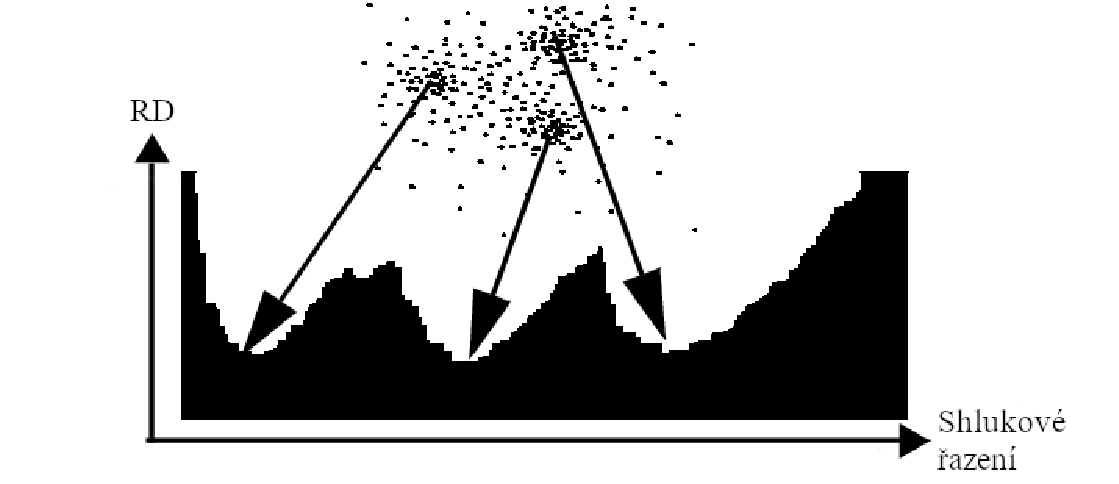
\includegraphics[width=0.9\textwidth]{obrazky/optics.pdf}
	\caption{Identifikace shluků z RD grafu (upraveno z~\cite{optics})}
	\label{optics-img}
\end{figure}

\section{Statistické metody}
Často k~detekci anomálií není třeba žádných zvláštních algoritmů a bohatě stačí statistické výpočty. Z~nich ostatně mnoho algoritmů vychází. Hlavní výhodou tohoto přístupu je jeho rychlost a jednoduchost. Na~druhou stranu má ale jen omezený rozsah použitelnosti.

\subsection{Pravděpodobnostní rozložení}
Předpokládají-li se data z~určitého rozložení pravděpodobnosti bez ohledu na~typ, lze velmi snadno detekovat outliery v~daném datasetu. Jednoduše stačí konkrétní datový bod dosadit do~příslušného vzorce, aby se zjistilo, zda do daného rozložení patří. Snadno lze výpočet modifikovat i pro~přidání případné tolerance.

Nechť se uvažuje například normální rozložení. To je definováno střední hodnotou \(\mu\) a směrodatnou odchylkou \(\sigma\). Pro toto rozložení platí pravidlo 3-sigma (obr.~\ref{3-sigma-img}), které říká, že cca 99.7~\% bodů Gaussova rozložení se nachází ve~vzdálenosti \(3\sigma\) od~jeho středu~\cite{3-sigma}. Z~toho vyplývá, že prakticky všechny vzdálenější body lze považovat za~outliery. Pravidlo \mbox{3-sigma} má navíc tu vlastnost, že vzdálenost \(2\sigma\) přibližně udává 95. percentil. Ten má mnoho využití v~různých sférách. Pro~některé aplikace umělé inteligence jím lze například čistit dataset od~outlierů. V~těch zbylých 5~\% se sice ještě nachází platná data, proto to nemusí být použitelné přímo pro~detekci, nicméně většinu outlierů to oddělá a chybějící krajní data, byť platná, kvalitu datasetu již tolik nemusí ovlivnit.

\begin{figure}[hbt]
	\centering
	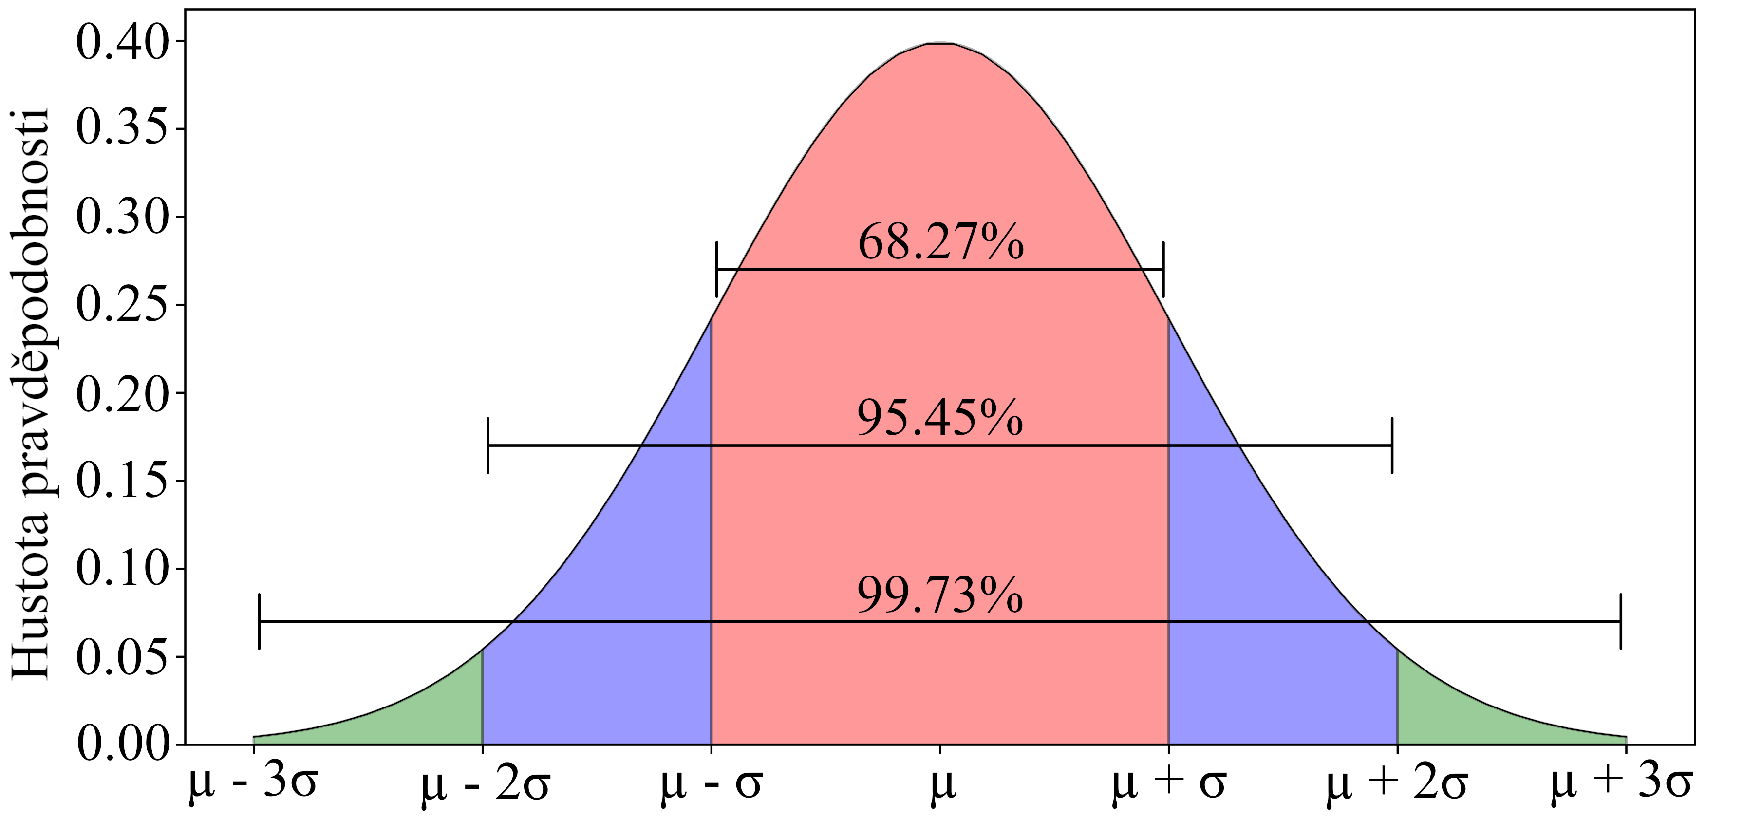
\includegraphics[width=0.85\textwidth]{obrazky/3-sigma.pdf}
	\caption{Pravidlo 3-Sigma Gaussova rozložení (upraveno z~\cite{3-sigma})}
	\label{3-sigma-img}
\end{figure}

\subsection{MAD}
Median Absolute Deviation (MAD), nebo-li medián absolutní odchylky, je velmi robustní statistické metoda využívaná k~měření variability dat~\cite{mad}. Lze ji vyjádřit jednoduchým vzorcem~\ref{mad-rovnice}:

\begin{equation}
\label{mad-rovnice}
MAD(X) = median({|x_i - median(X)|})
\end{equation}

V~podstatě se jen vypočítá medián datasetu X, pro~každou hodnotu x\textsubscript{i} z~datasetu X se spočítá odchylka od~onoho mediánu a jako výsledek se vezme medián absolutních hodnot těchto odchylek~\cite{mad}. V~detekci anomálií se často využívá pro~porovnávání časových řad~\cite{mad}. Jestliže se MAD bodu některé řady liší v~porovnání s~body v~ostatních řadách ve~stejném časovém úseku o~více než předem stanovenou mez, lze bod považovat za~outlier. Pokud řadu tvoří více než určité procento outlierů, celá řada je pak outlier.

\subsection{Z-skóre a modifikované z-skóre}
Z-skóre lze vnímat jako standardizované normální rozložení určitého datasetu se vzorcem~\ref{zscore-rovnice}. Vyjadřuje odchýlení jednotlivých bodů od~průměru v~jednotkách směrodatné odchylky.

\begin{equation}
\label{zscore-rovnice}
Z = \dfrac{X - \mu}{\sigma}
\end{equation}

Jeho nepřesnost však spočívá v~tom, že outliery silně ovlivňují nejen průměrnou hodnotu, nýbrž i směrodatnou odchylku. Tento problém řeší tzv.~modifikované z-skóre, které používá robustnější parametry, konkrétně tedy medián místo průměru a MAD místo směrodatné odchylky~\cite{z-score}. Výsledek pak ještě dle vzorce~\ref{modifikovane-zscore-rovnice} násobí normalizační konstantou 0.6745~\cite{z-score}.

\begin{equation}
\label{modifikovane-zscore-rovnice}
Z = 0.6745\times\dfrac{X - median(X)}{MAD(X)}
\end{equation}

Dále je pouze třeba vymezit hraniční skóre, nad~kterým budou prvky považovány za~outliery. Cena za~rychlost, robustnost a jednoduchost této metody je však předpoklad alespoň přibližného normálního rozložení zpracovávaných dat.

\section{Rozhodovací stromy}
Typickým použitím rozhodovacích stromů je klasifikační nebo regresní analýza objektů na~základě jejich vlastností. Strom se vytváří dělením zdrojové množiny dle hodnot parametrů jejích objektů na~podmnožiny, jež se stávají zdrojovými množinami pro~další větvení~\cite{decision-trees}. Výběr vhodných parametrů pro~co nejúčinější dělení se provádí specifickou funkcí pro~daný problém. Častým způsobem je například výpočet tzv.~informačního zisku na~základě entropie~\cite{decision-trees}. Rozhodovací stromy jsou jednou z~nejstarších a nejběžnějších metod pro~získání informací z~dat nejen v~oblasti strojového učení. Jak je však lze využít k~detekci anomálií?

\subsection{Isolation forest}
\label{isolation-forest}
Tvůrci algoritmu Isolation forest (česky izolační les) ve své studii \cite{isolation-forest} tvrdí, že většina algoritmů pro~detekci anomálií pracuje na~tom způsobu, že si definují, co~je normální, a za~anomálie prohlašují ta data, jež nesplňují daná kritéria. Tyto algoritmy jsou pak podle nich optimalizované právě pro~úkol najití běžného chování, nikoliv však pro~samotnou detekci anomálií. Další nevýhodu vidí v~omezení na~nízkodimenzionální data z~důvodu výpočetní složitosti.
K~problému proto přistupují obráceně a algoritmus navrhují tak, aby se již přímo zaměřoval na~vyčlenění anomálních dat. Toho lze dosáhnout zaměřením se na~jejich obecné vlastnosti, tedy že jich je málo a jsou nějakým způsobem odlišné.

Princip fungování algoritmu není příliš složitý. Jeho cílem je odizolovat jednotlivé prvky z~datové množiny. Nechť se vezme v~úvahu dataset vykreslený na obrázku~\ref{isolation-forest-splitting-img}. Pro~každý bod se náhodně zvolí dimenze a místo, ve~kterém se provede řez, čímž se rozštěpí strom na~dvě větve~\cite{isolation-forest}. Štěpení se dále provádí, dokud se prvek neodizoluje, nebo dokud není dosaženo předem stanovené maximální výšky stromu~\cite{isolation-forest}. Anomální prvky k~odizolování potřebují méně řezů než platné.

\begin{figure}[hbt]
	\centering
	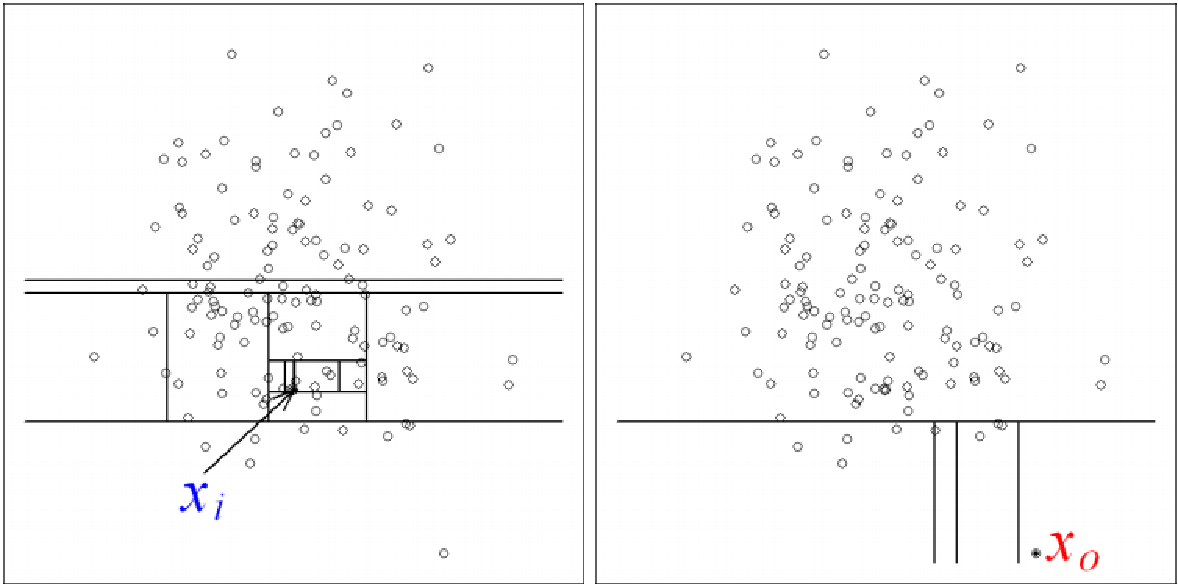
\includegraphics[width=1\textwidth]{obrazky/isolation-forest-splitting.pdf}
	\caption{Izolování prvků náhodnými řezy v~algoritmu Isolation forest (převzato z~\cite{isolation-forest})}
	\label{isolation-forest-splitting-img}
\end{figure}

Anomálie se však mohou vyskytovat ve~shlucích nebo blízko platných dat. V~takovém případě by výše zmíněný postup nebyl moc efektivní. Zde proto přichází do~hry tvorba lesa. Dataset se podvzorkuje, čímž se zmenší význam shluků a zvýrazní izolace (obr.~\ref{isolation-forest-subsampling-img})~\cite{isolation-forest}. Algoritmus se pak provádí nad~těmito redukovanými datasety. Ve~výsledku tak vzniká několik stromů (les), který každý dává vlastní výsledek. To má ty pozitivní vlastnosti, že se výrazně potlačuje přetrénování, jež zcela jistě u~některých stromů nastane, ale ne u~všech a u~každého třeba v~jiném směru. Dále je model přesnější, neboť vícero stromů se musí shodnout na~výsledku~\cite{isolation-forest}.

\begin{figure}[hbt]
    \centering
    \subfloat[\centering Původní data]{{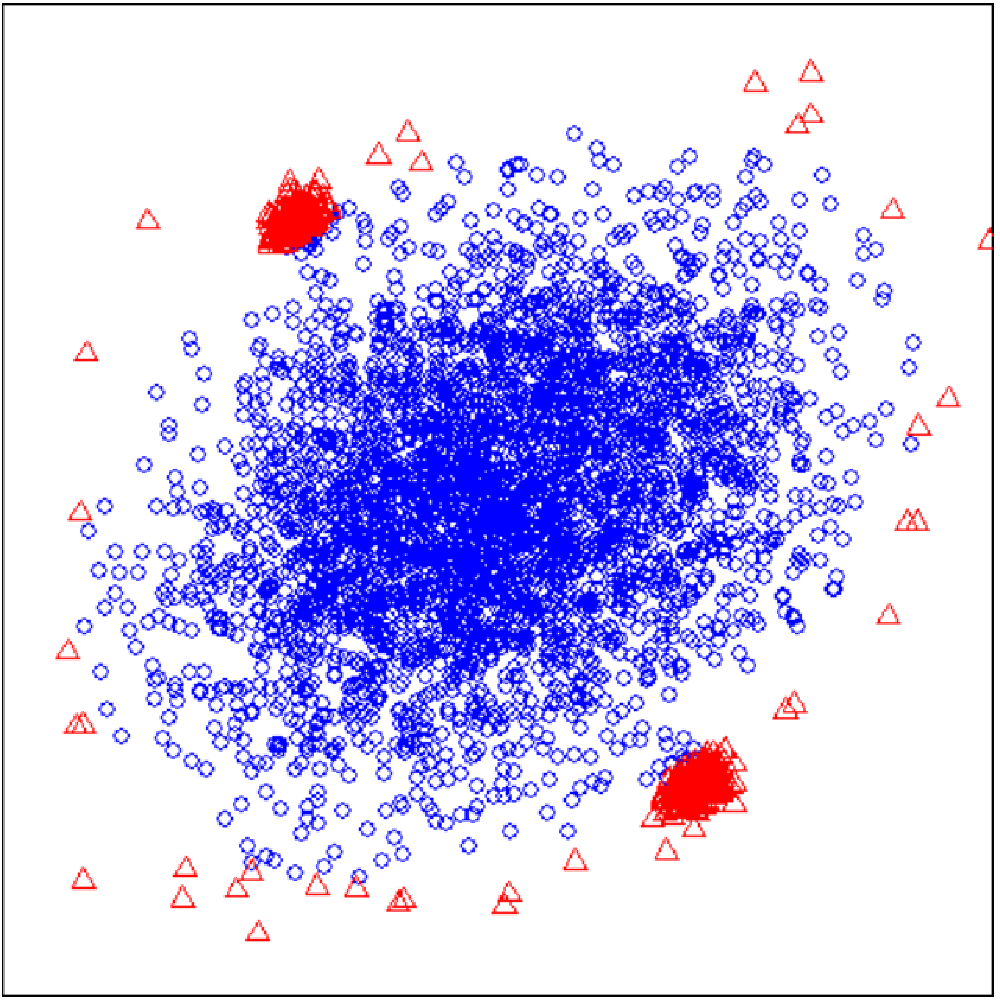
\includegraphics[width=7cm]{obrazky/isolation-forest-subsampling-1.pdf} }}
    \qquad
    \subfloat[\centering Podvzorkovaná data]{{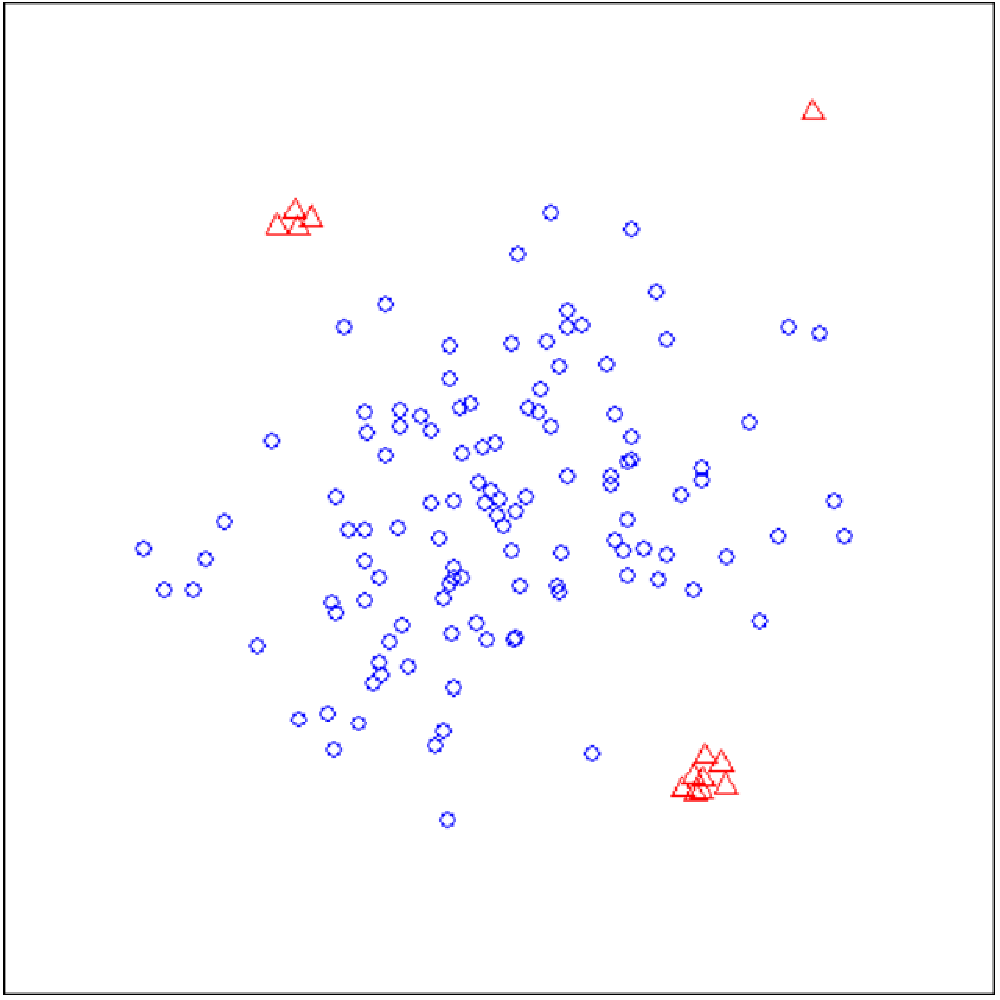
\includegraphics[width=7cm]{obrazky/isolation-forest-subsampling-2.pdf} }}
    \caption{Podvzorkovaná data snáze vytyčí anomální body (převzato z~\cite{isolation-forest}).}
    \label{isolation-forest-subsampling-img}
\end{figure}

Samotné rozhodnutí o~anomálii se provádí měkce pomocí skóre každého prvku. To závisí na~počtu řezů, tedy délce cesty k prvku ve~stromu. Hodnota skóre se pohybuje v~intervalu \(<0,1>\), lze proto snadno uvádět procentuální míru anomálnosti prvku. Dle aplikace se jen určí vhodná hranice. Práce \emph{Isolation Forest}~\cite{isolation-forest} vysvětluje skóre následovně. Prvek se skóre blízkým 1 je zcela jistě outlier. Výrazně nižší skóre než~0.5 pak indikuje naprosto běžný prvek. Jestliže však mají všechny prvky skóre blízké 0.5, pak celý dataset nevykazuje žádné výrazné anomálie.

Předními vlastnostmi algoritmu Isolation forest jsou podle literatury~\cite{isolation-forest} jeho lineární časová složitost a velmi nízké paměťové nároky. Dále se uvádí jeho vysoká rychlost v~porovnání s~jinými algoritmy, neboť nepočítá žádné vzdálenosti. Díky podvzorkování pak dokáže zpracovat velmi velká nebo i vysokodimenzionální data. V~neposlední řadě je mnohem snazší volba parametrů algoritmu než je tomu u~jiných metod. Stačí specifikovat pouze počet stromů a jejich velikost, přičemž oba tyto parametry již mají empiricky ověřené vhodné hodnoty.

  \chapter{Návrh a implementace modelu strojového učení pro detekci anomálií}
\label{navrh-ai}

Pojem anomálie se různí s~každou aplikací. Sekce~\ref{anomalie-v-rqa} se proto zabývá definicí anomálie v~RQA a tedy tím, co se v~datech přesně hledá. Dále je stručně shrnuto, jaká data jsou k~dispozici a co to pro~strojové učení znamená. Je proveden návrh detekce anomálií v~délkách zpracování požadavků s~ohledem na~algoritmy popsané v~kapitole~\ref{ml-algoritmy}. V~rámci něj je vyzkoušeno a zhodnoceno několik kandidátních algoritmů. Následuje návrh detekce anomálií v~počtech chyb během požadavků. Kapitola dále představuje implementační řešení návrhů obou detekcí anomálií. Na~závěr je ukázána tvorba referenčního datasetu se~způsobem zachování jeho čistoty při~příchodu nových dat.

\section{Anomálie v RQA systému}
\label{anomalie-v-rqa}
Anomálie bývá velmi často zaměňována s~pojmem outlier~\cite{anomaly-vs-outlier-book, anomaly-vs-outlier-post}. V~závislosti na~typu aplikace či problému však tato záměna může i nemusí být korektní. Anomálie typicky značí výskyt dat, která jsou nějakým způsobem špatná či neplatná~\cite{anomaly-vs-outlier-post}. Outlier na~druhou stranu označuje prvek, jenž se výrazně liší od~ostatních v~dané kolekci~\cite{anomaly-vs-outlier-post}. Nemusí se však nutně jednat o~neplatný prvek, pouze odlišný. Z~těchto definic je patrné, že outlier někdy anomálií být může a někdy~ne. Dochází-li tedy k~vzácnému výskytu outlierů nebo jsou tyto nějakým způsobem významné, mohou být rovnou označeny za~anomálie. Pokud je však jejich přítomnost zcela běžná, budou spíše vnímány jako přirozený šum v~datech.

Délka zpracování síťových požadavků obecně nebývá zcela stabilní. K~občasným zdržením dochází, a musí se s nimi proto počítat. Outliery jsou tedy z~pohledu RQA běžnou záležitostí a jedná se o~platná data. Problém nastává až v~okamžiku, kdy se outliery opakují, tedy pokud zpracování některého požadavku trvá opakovaně nezvyklou dobu. Anomálií v~délkách zpracování požadavků se proto rozumí výraznější shluk outlierů. Mezi počty chyb, kde již není taková různorodost hodnot, lze za~anomálii považovat změnu v~chybovosti přesahující předem určenou mez. V~obou případech se anomálií vnímá i pozitivní změna. Skutečnost, že některá služba běží rychleji nebo s~méně chybami je samozřejmě dobré znamení, nicméně stále se jedná o~nestandardní výskyt. Může být proto vhodné vyšetřit i tuto situaci. Buď se na~základě této změny mohou vylepšit i jiné části systému, nebo se třeba odhalí chyba v~toku programu.

\section{Vlastnosti nasbíraných dat}
\label{vlastnosti-nasbiranych-dat}
Sběr dat popsaný kapitolou~\ref{sber-dat} poskytuje algoritmům data pro~každou službu v~CSV souborech. Konkrétně se na~straně detekční aplikace vyskytuje adresář s~daty, v~němž má každá služba vlastní složku. V~té se nachází CSV soubor pro~každý typ požadavku dané služby. Uvnitř takového souboru pak lze najít záznamy o~jednotlivých požadavcích obsahující časové razítko, délku zpracování požadavku a počet chyb během požadavku. Časová známka není podstatná pro~samotnou detekci, nicméně požadavek identifikuje, je díky ní možné uchovávat data jen po~určitou dobu a dobře slouží k~vizualizaci výsledků. Detekce poté probíhá zvlášť nad~délkami zpracování požadavků a zvlášť nad~počty chyb. Vstupní data algoritmů jsou tedy jednodimenzionální. Tento fakt přináší několik výhod:

\begin{itemize}
    \item Jednodimenzionální rozměr je pro~člověka zcela přirozený a lehce představitelný.
    \item Výpočty nad takovými daty jsou velmi rychlé.
    \item Výrazně se sníží paměťové nároky na~výpočet.
    \item Je možné je snadno vizualizovat a to nejen ve~své dimenzi, ale i například v~závislosti na čase daným časovým razítkem.
    \item Návrh či budoucí úprava algoritmů nad těmito daty je mnohem snazší a rychlejší. Výběr algoritmů je taktéž širší, neboť nehrozí omezení dimenzionalitou dat.
\end{itemize}

U~délek zpracování požadavků bylo navíc z~nasbíraných dat vypozorováno jejich pravděpodobnostní rozložení. Obrázek~\ref{data-img} zobrazuje několik zástupců typických dat.

\begin{figure}[hbt]
    \centering
    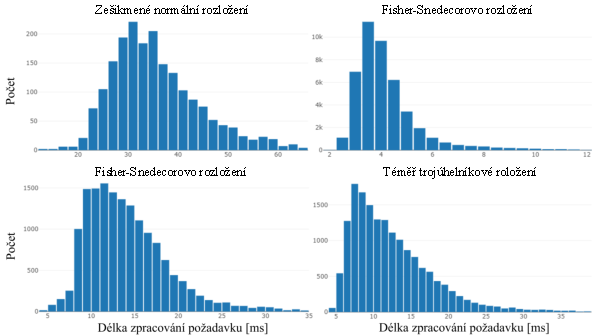
\includegraphics[width=1\textwidth]{obrazky/rqa-data-distribution.pdf}
    \caption{Rozložení délky zpracování požadavků vychází z~normálního rozložení. To však nikdy není čisté, nýbrž kladně zešikmené. Nejčastěji proto připomíná spíše Fisher–Snedecorovo různých volností. V~krajním případě má i tvar trojúhelníku. Rozložení je tedy poměrně různorodé, nicméně vždy se drží mezi normálním a trojúhelníkovým.}
    \label{data-img}
\end{figure}

\section{Detekce anomálií v~délkách zpracování požadavků}
\label{detekce-anomalii-v-delkach-pozadavku}
Jak již bylo zmíněno v podkapitole \ref{anomalie-v-rqa}, cílem je najít shluky mezi outliery. Pro tuto úlohu se nabízí dvě možné řešení. Prvním je aplikace shlukování na celý dataset. Toto řešení však obsahuje zásadní nedostatek, jenž vysvětluje sekce~\ref{shlukova-analyza-nad-kolekci-dat}. Druhou možností je problém rozdělit na~podproblémy. Takový přístup je mnohem flexibilnější a již umožňuje řešit zadanou úlohu. Rozdělení na~podproblémy nejen že rozšiřuje škálu použitelných algoritmů, nýbrž i zjednodušuje hledání jejich parametrů, neboť cíle algoritmů jsou jednodušší. V~první fázi se proto pouze oddělí outliery od~platných dat. Následně se provede shluková analýza nad~těmito outliery. V~posledním kroku se už jen pro každý shluk outlierů rozhodne, zda-li je dostatečně velký pro~označení za~anomálii. Důležité je si však uvědomit, že se nelze zaměřit na~konkrétní data, na~nichž lze perfektně odladit parametry jednotlivých algoritmů. Detekci je potřeba  navrhnout v~obecnosti, aby byla schopna pracovat nad~libovolnými daty popsanými v~předchozí podkapitole.

\subsection{Shluková analýza nad~celou kolekcí dat}
\label{shlukova-analyza-nad-kolekci-dat}
Myšlenka tohoto přístupu je taková, že by se provedlo shlukování nad~celým datasetem a za~anomálie by pak bylo možné považovat krajní shluky. Hlavní výhodou je, že by stačil pouze jeden průchod daty jediným shlukovacím algoritmem. Ten je nutné hledat mezi algoritmy založených na hustotě. Důvodem je dopředná neznalost počtu anomálií, tedy shlukovacích tříd. Zároveň je žádoucí ignorovat osamocené outliery, nebo-li šum, na~což jsou tyto algoritmy dobré. Další důležitou vlastností algoritmu musí být schopnost rozpoznat shluky odlišných hustot, neboť jinak hustý bude hlavní shluk obsahující platná data a jinak pak anomální shluky. Z~algoritmů představených kapitolou~\ref{ml-algoritmy} splňují tyto vlastnosti HDBSCAN a OPTICS. Problém však spočívá v~tom, že není možné najít vhodné parametry vybraných algoritmů. Obrázky~\ref{direct-detection-soft-img} a~\ref{direct-detection-hard-img} znázorňují paradox ve~hledání parametrů. 

\begin{figure}[hbt]
    \centering
    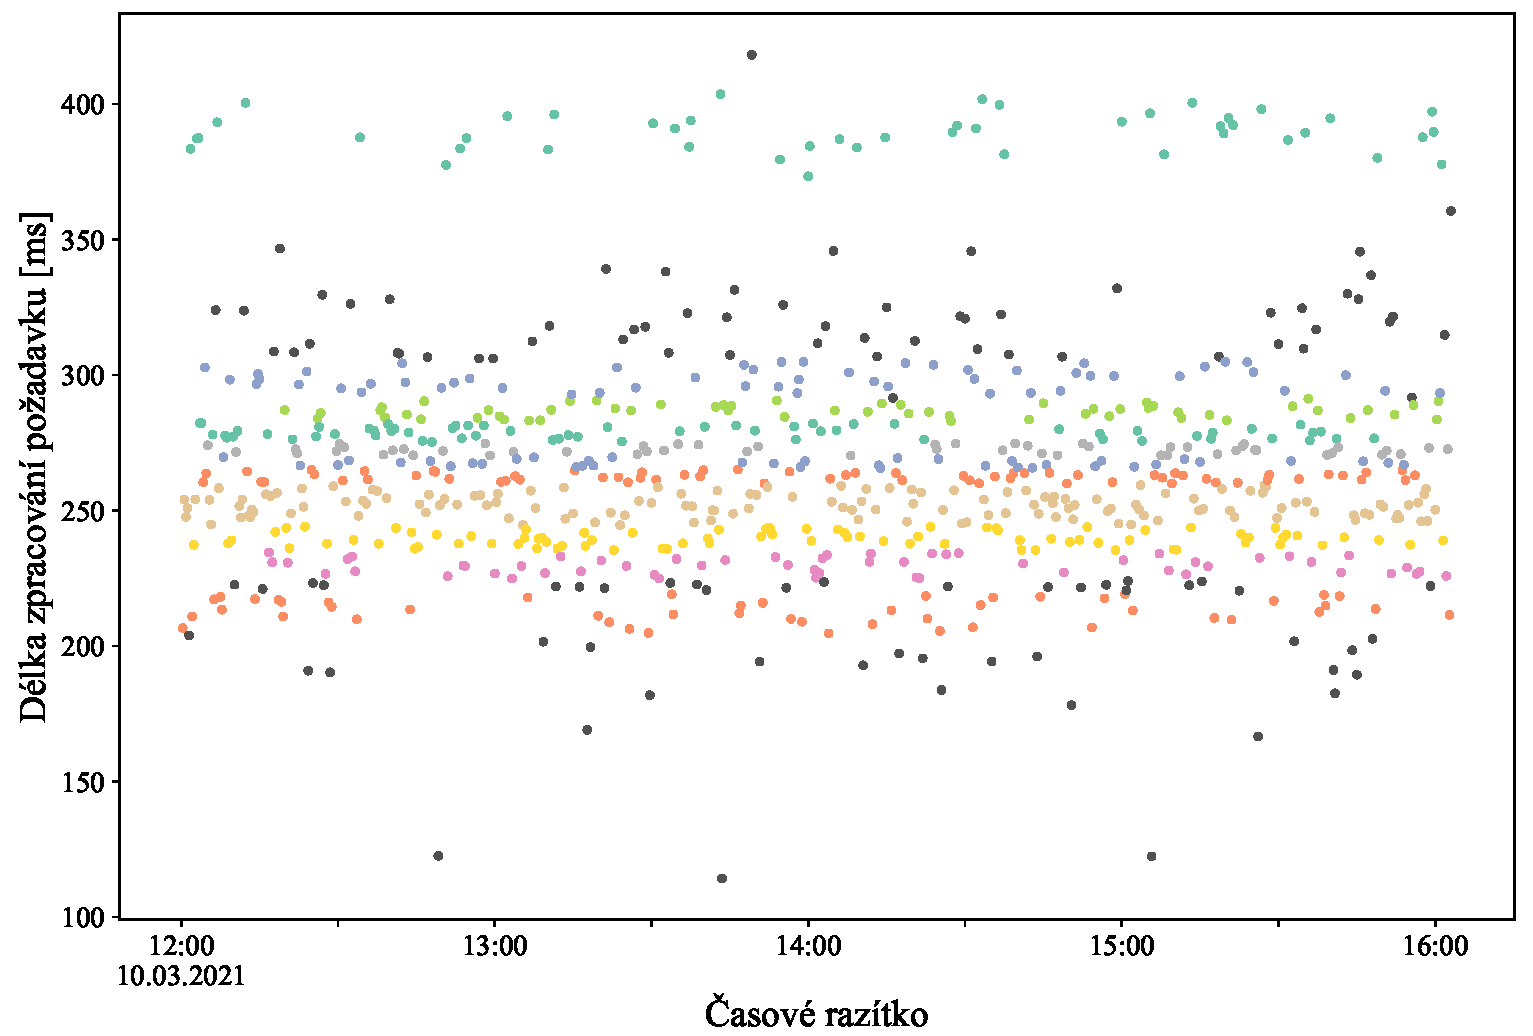
\includegraphics[width=0.88\textwidth]{obrazky/direct-detection-soft.pdf}
    \caption{Nízké nároky na shluk rozštěpí hlavní shluk na~mnoho podshluků.}
    \label{direct-detection-soft-img}
\end{figure}

\begin{figure}[hbt]
    \centering
    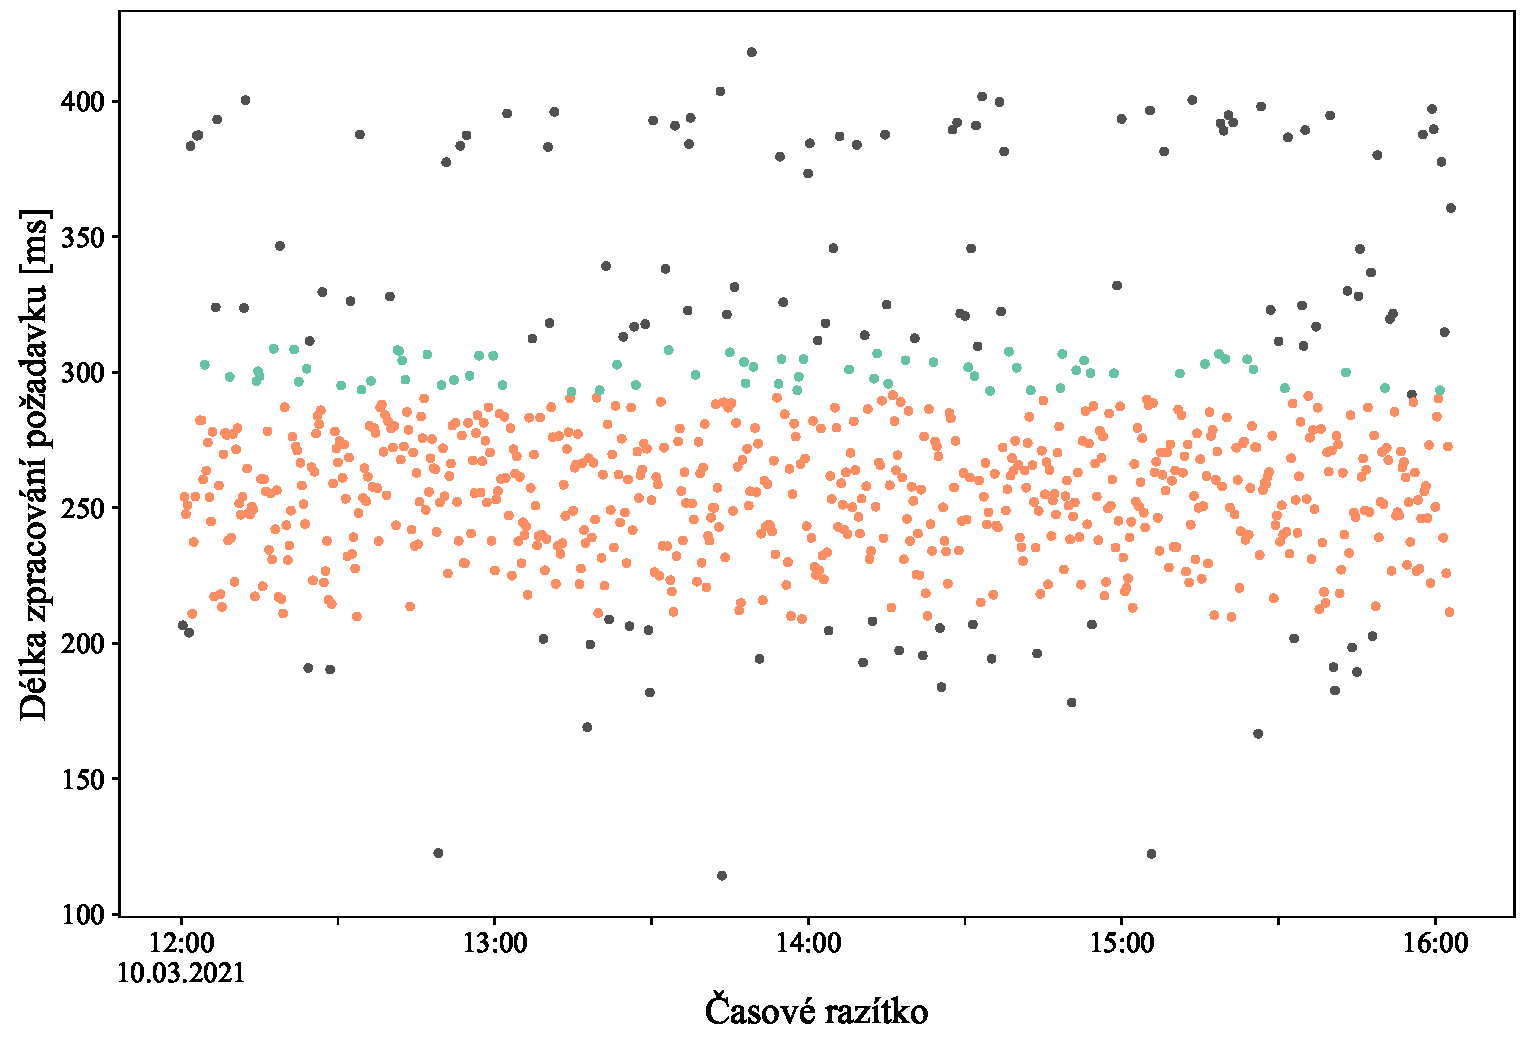
\includegraphics[width=0.88\textwidth]{obrazky/direct-detection-hard.pdf}
    \caption{S~velkými nároky na~shluk není anomálie ani jako shluk rozpoznána.}
    \label{direct-detection-hard-img}
\end{figure}

Na~obou obrázcích lze spatřit anomálii blízko hodnoty 400~ms. Vzhledem k~tomu, že anomální shluky jsou typicky menší a okrajové, je třeba zvolit parametry dostatečně jemně, aby shluky byly rozpoznány. Jak však ukazuje obrázek~\ref{direct-detection-soft-img}, nízké požadavky na~shluk způsobí, že se i hlavní shluk rozštěpí na~mnoho menších, neboť tyto také splňují specifikace shluku. Při~snaze tento problém kompenzovat zpřísňováním požadavků na~shluk nastane situace jako na~obrázku~\ref{direct-detection-hard-img}, na němž již anomální shluk není dostatečně hustý či velký na~to, aby byl za~shluk vůbec považován.

\subsection{Detekce outlierů}
\label{detekce-outlier}
Kapitola~\ref{ml-algoritmy} představila několik algoritmů, které jsou vhodnými kandidáty pro~tento úkol. V~první řadě lze opět použít algoritmy založené na~hustotě. Zde se již hledání parametrů značně zjednoduší, neboť stačí rozlišit jen jeden hlavní shluk platných dat od~šumu. Vzhledem ke~zrušení variability hustoty je výhodné použít základní variantu DBSCAN.

Pro~získání vhodných parametrů byly prováděny experimenty nad~normálním rozložením, jež zobrazuje tabulka~\ref{dbscan-params-table}. Dobrými hodnotami se projevily být číslo~5 pro parametr MinPts a číslo 25 pro~\textepsilon. V~případě, že by dataset obsahoval méně prvků, než dvojnásobek~\textepsilon, tedy~50, je za~\textepsilon~zvolena polovina velikosti datasetu. Vybrané parametry však ještě byly testovány způsobem popsaným v~sekci~\ref{testovani-konkretni-anomalie}, neboť zmíněné experimenty vedly pouze k~získání výchozích hodnot, kolem kterých by se parametry mohly pohybovat. Pro~jiné směrodatné odchylky nebo i jiná rozložení tyto parametry nemusely být optimální. Testování však prokázalo, že nepracují špatně ani s~jinými typy dat, a~proto byly nakonec použity. Obrázek~\ref{dbscan-outlier-detection-img} ukazuje výsledek aplikace DBSCAN algoritmu s~těmito parametry.

\begin{figure}[hbt]
    \centering
    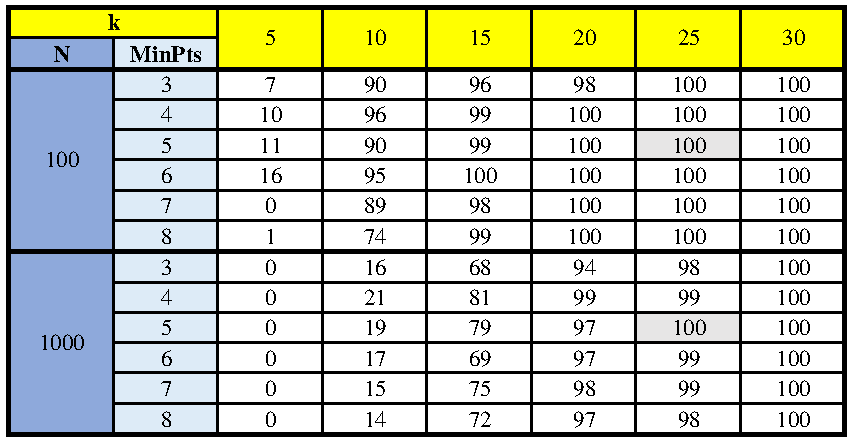
\includegraphics[width=0.935\textwidth]{obrazky/dbscan-params-results.pdf}
    \caption{Tabulka ukazuje výsledky experimentů DBSCAN algoritmu s~různými parametry. Pro~každou kombinaci bylo provedeno 100 pokusů nad~náhodnými daty normálního rozložení se~směrodatnou odchylkou \(\sigma = 15\). Číslo udává počet přijatelných oddělení outlierů od~platných dat zkontrolovaných člověkem. N~zde značí počet prvků rozložení, neboť jinak se algoritmus chová nad~malými a velkými datasety. Písmeno k je \emph{k}-tý soused, vzdálenost k~němuž se použila jako \textepsilon}
    \label{dbscan-params-table}
\end{figure}

\begin{figure}[!hbt]
    \centering
    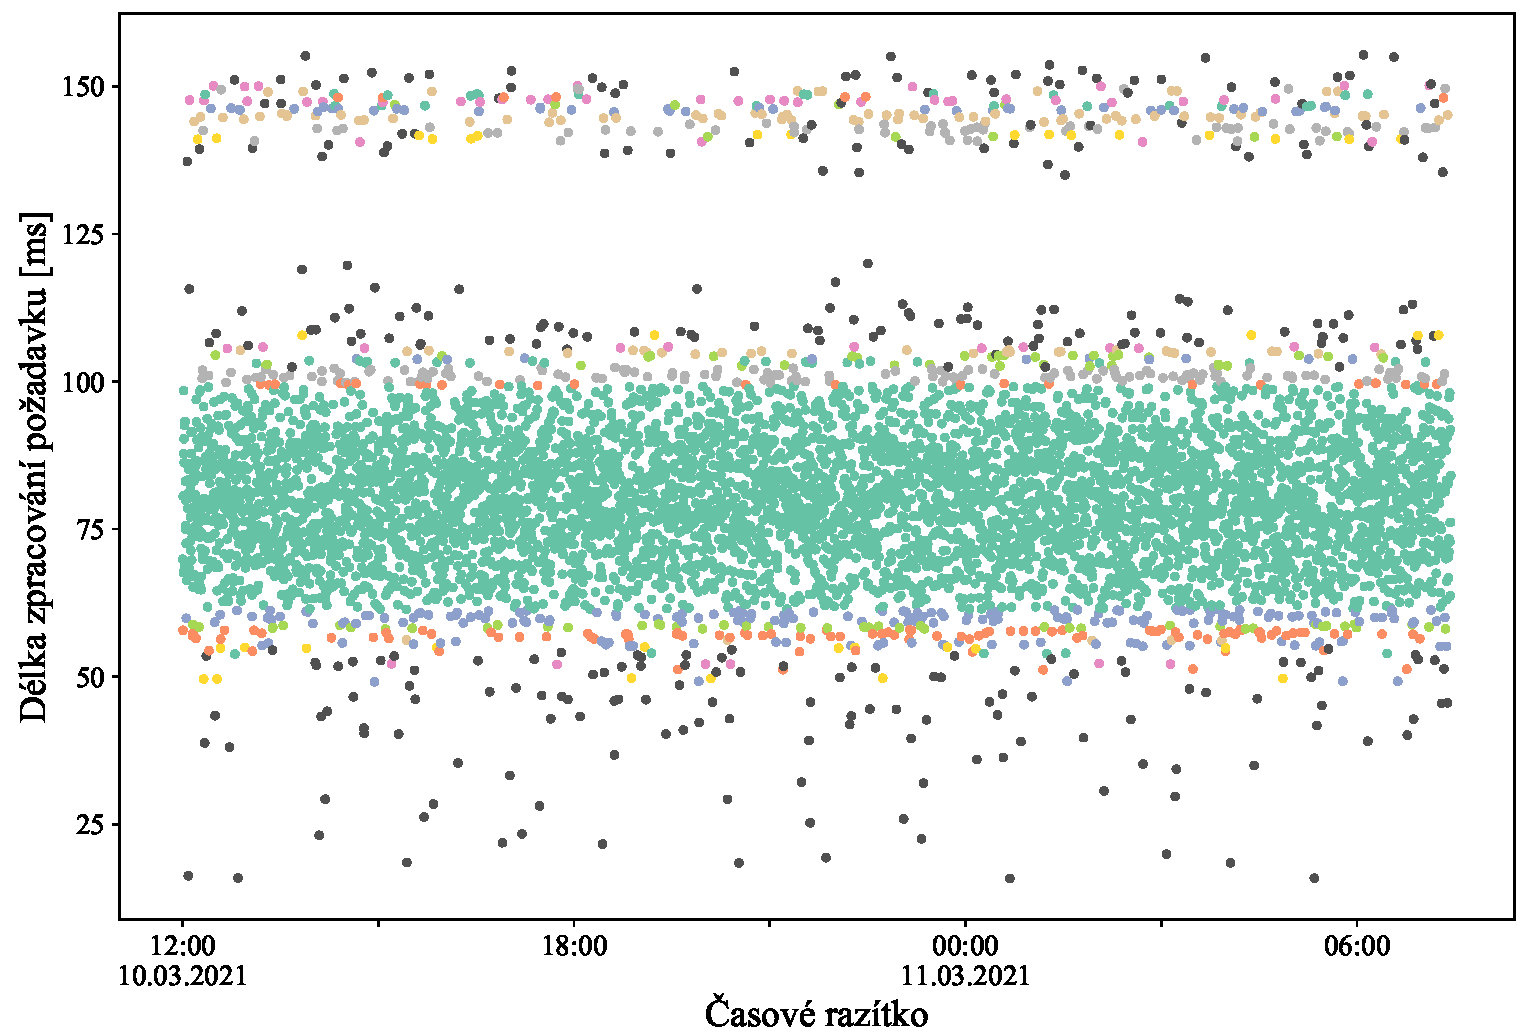
\includegraphics[width=0.935\textwidth]{obrazky/dbscan-outlier-detection.pdf}
    \caption{Za~outliery se v~tomto výsledku DBSCAN algoritmu považuje vše, co nepatří do~hlavního zeleného shluku.}
    \label{dbscan-outlier-detection-img}
\end{figure}

DBSCAN ve~většině případů spolehlivě nalezne hlavní shluk, nicméně jak je vidět, nezahrne velké množství okrajových dat, které by měly být součástí. Přesnost tohoto velmi závisí na konkrétním rozložení. Další problém spočívá v~tom, že u~velmi malých datasetů a ještě s~nepříznivým rozložením občas nenalezne žádné shluky, což není přijatelné.

Další možností je algoritmus Isolation forest, který je přímo optimalizován na~detekci outlierů. Za~parametry byly zvoleny doporučené hodnoty 100 stromů v~lese a 256 vzorků pro~strom~\cite{isolation-forest}. Nalezení hraničního skóre, které by bylo použitelné v~obecnosti, však nebylo možné. Silně totiž závisí na~počtu a hustotě dat. Obrázek~\ref{iForest-outlier-detection-img} zobrazuje případ, kdy je anomálie poměrně hustá a mnoho anomálních dat je považováno za platná. Tento jev je možné odstranit zpřísněním skóre, nicméně přišlo by se tím o~značné množství krajních platných dat. Navíc se nejedná ani o~žádný extrémní případ. Pokud by anomálie byla dostatečně velká a hustší než platná data, budou mít její prvky nižší skóre a nebude možné je vůbec oddělit. Ukázalo se tedy, že Isolation forest by byl vhodný na~odstranění šumu, nicméně nelze ho v~obecnosti využít pro~vytyčení hlavního shluku v~datech.

\begin{figure}[!hbt]
    \centering
    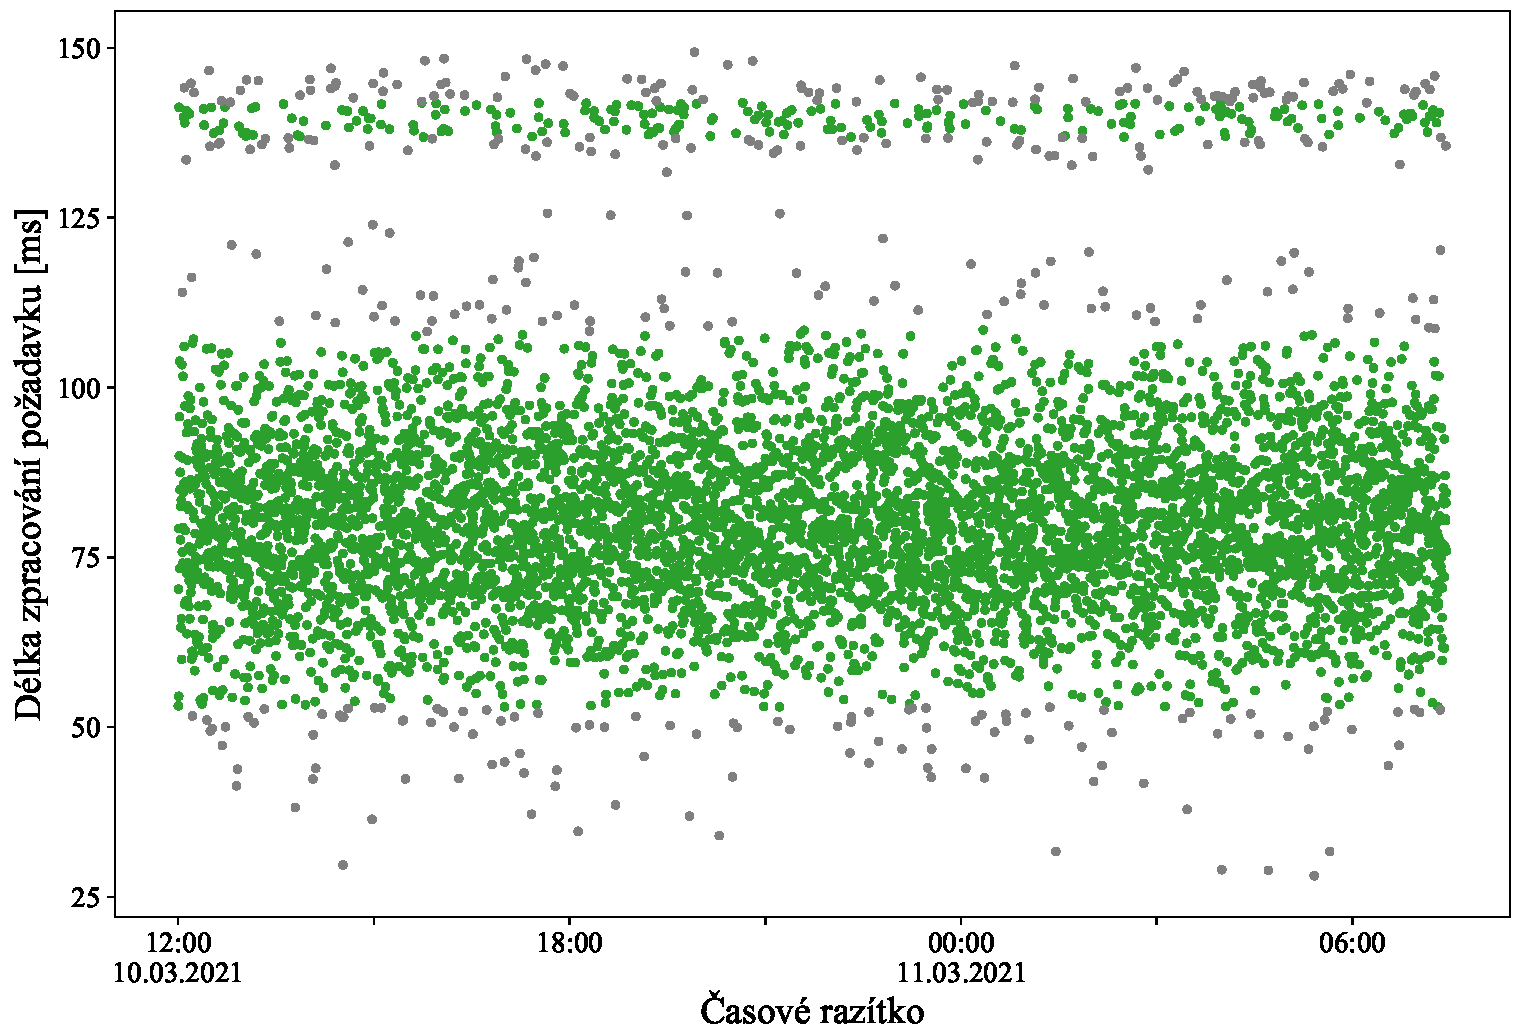
\includegraphics[width=0.88\textwidth]{obrazky/iForest-outlier-detection.pdf}
    \caption{Výsledek algoritmu Isolation forest pro~detekci outlierů}
    \label{iForest-outlier-detection-img}
\end{figure}

Jednodimenzionalita dat a jejich víceméně normální rozložení umožňuje použít i statistickou metodu modifikované z-skóre. Z~výše uvedených je nejrychlejší a vyžaduje pouze jeden parametr. Tím je hraniční skóre, nad~nímž jsou data považována za~outliery. Dobrou hranicí se ukázalo být skóre 2.35, jak lze částečně vypozorovat z~obrázku~\ref{z-score-param-img}. Výchozím hraničním skórem byla hodnota 3, jež bývá často používána~\cite{z-score}. Pro čisté normální rozložení je velmi dobrá, nicméně u~strmějších rozložení (Fisher-Snedecorovo, trojúhelníkové) může zahrnout i mnoho outlierů. Podobným problémem trpí i hodnota 2.5. Přísnější hranice, jakou je třeba číslo 2, se tohoto nedostatku zbavuje, nicméně již zase ořezává dost dat na~druhé straně rozložení. Jako kompromis byla zpočátku zvolena hodnota 2.3, jež byla během testování dle sekce~\ref{testovani-konkretni-anomalie} upravena na 2.35.

\begin{figure}[!hbt]
    \centering
    \subfloat[\centering Normální rozložení]{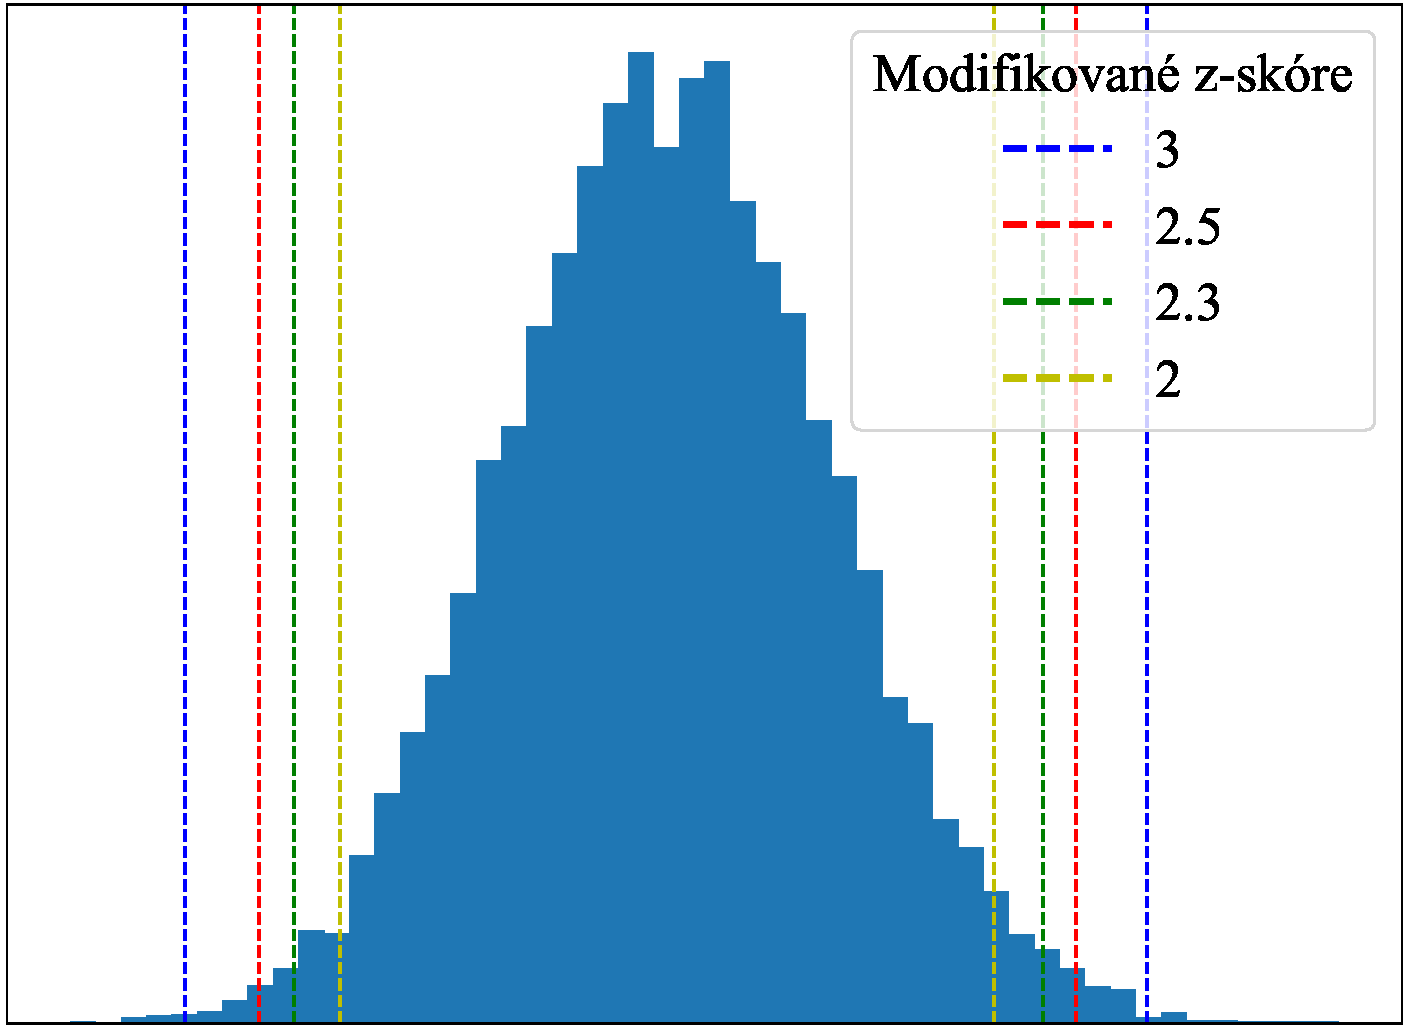
\includegraphics[width=0.49\textwidth]{obrazky/z-score-normal.pdf}}
    \subfloat[\centering Fisher-Snedecorovo rozložení]{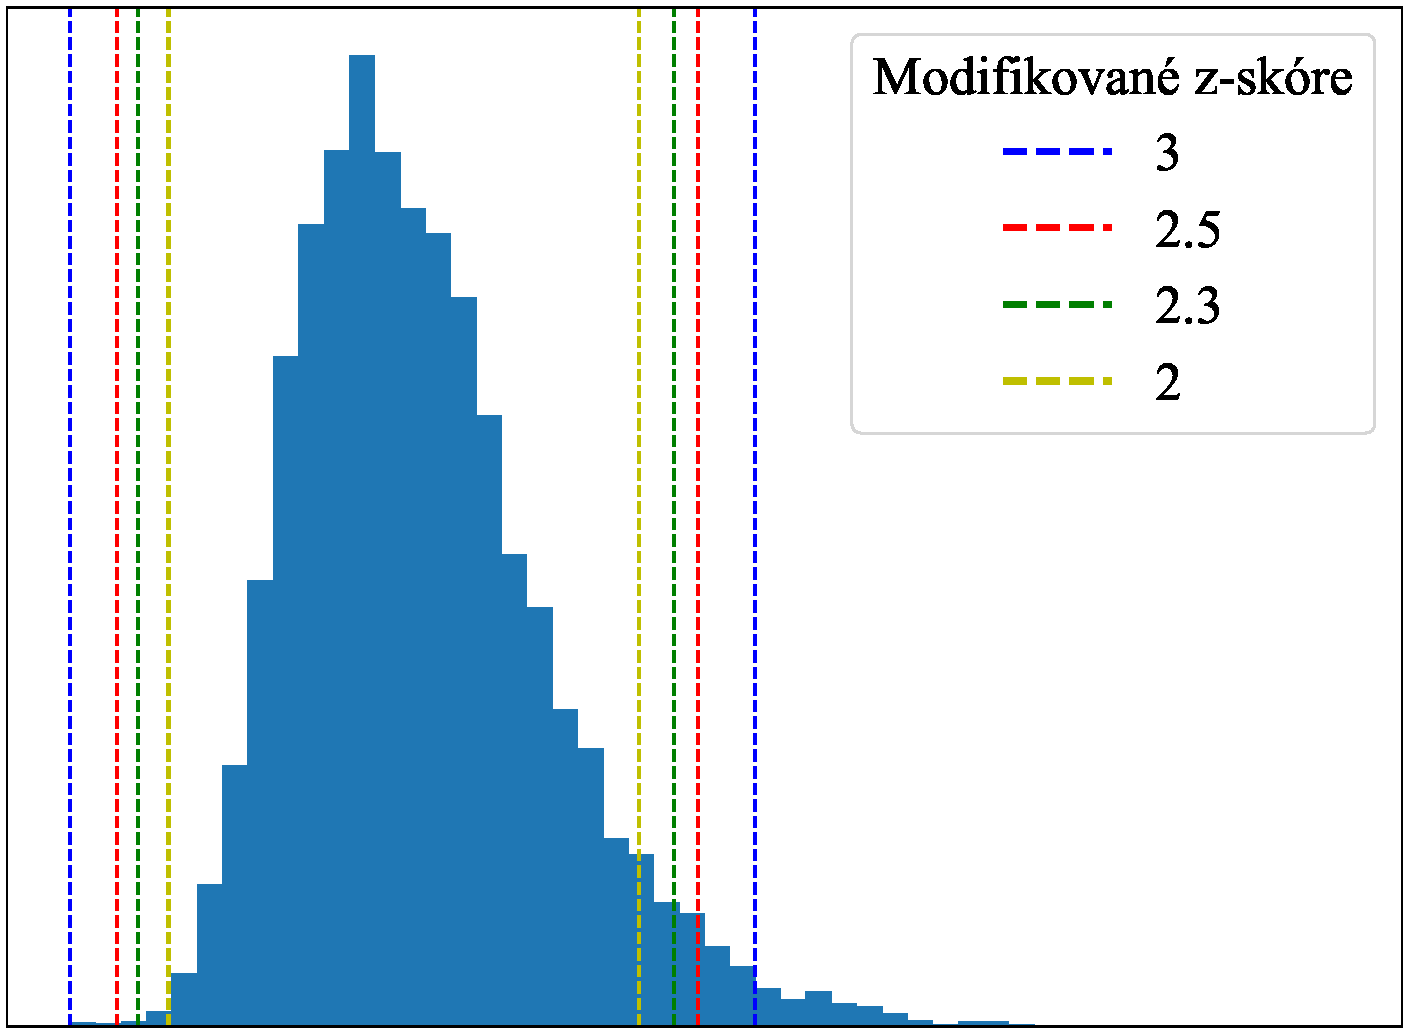
\includegraphics[width=0.49\textwidth]{obrazky/z-score-f.pdf}}
    \qquad
    \subfloat[\centering Trojúhelníkové rozložení]{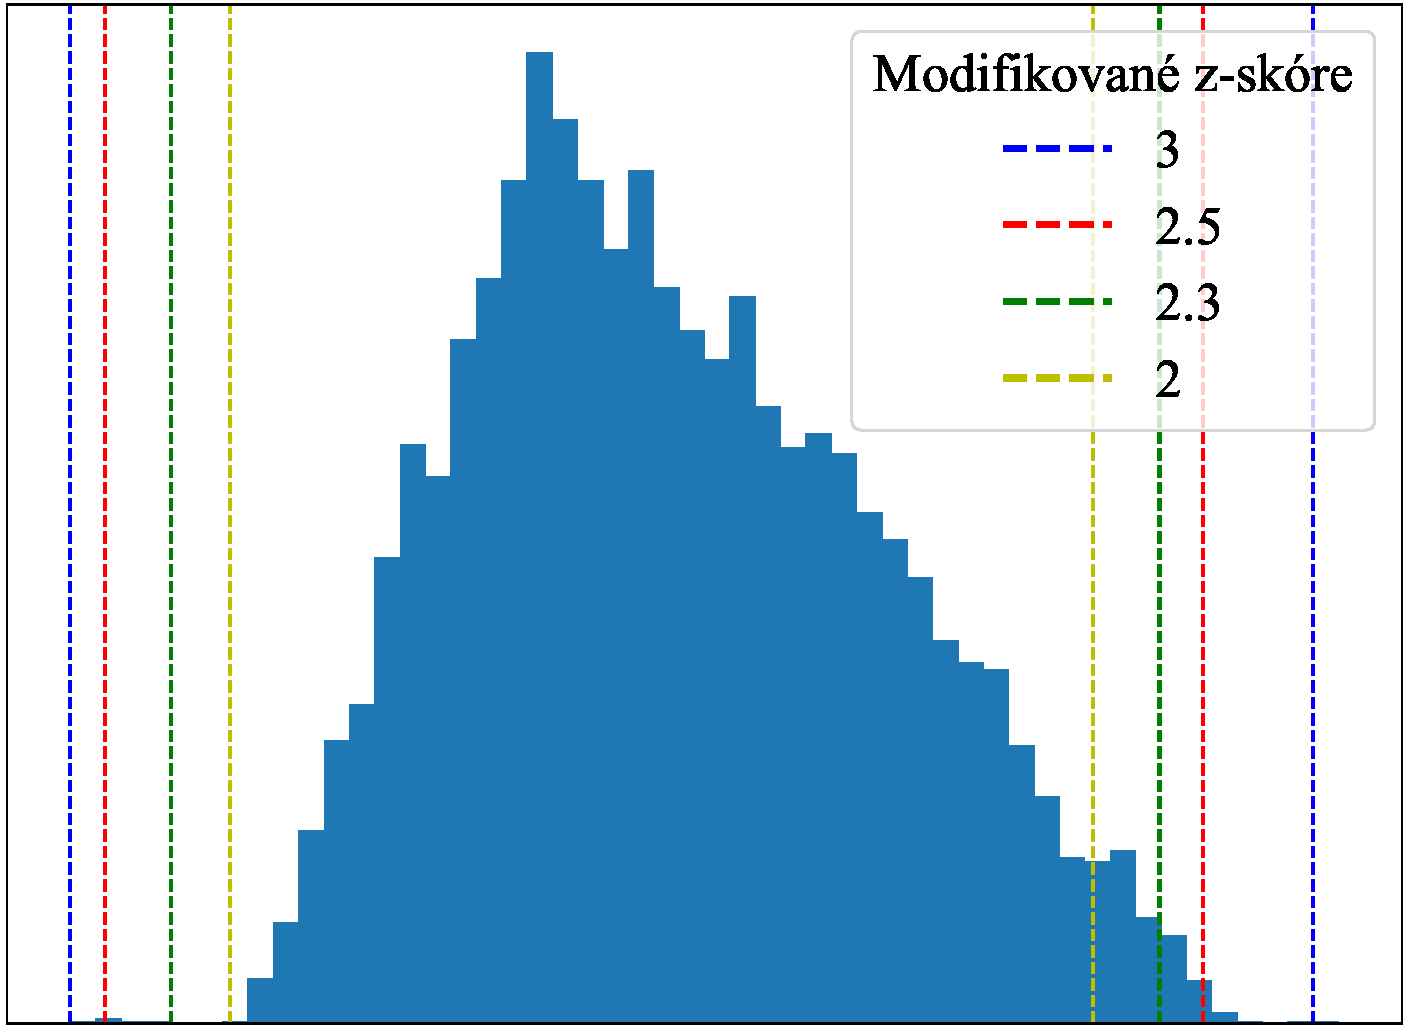
\includegraphics[width=0.49\textwidth]{obrazky/z-score-triangular.pdf}}
    \caption{Hranice modifikovaného z-skóre různých rozložení}
    \label{z-score-param-img}
\end{figure}

Na~obrázku~\ref{modified-zscore-outlier-detection-success-img} pak lze vidět velmi přesné oddělení platných dat a outlierů. Navzdory kvalitním výsledkům však ani metoda modifikovaného z-skóre není perfektní. Čím více se totiž rozložení dat vzdaluje od~normálního, tím větší počet krajních platných dat se odřízne. V~porovnání s jinými algoritmy však toto není nic neobvyklého. Ať už se rozhoduje na~základě hustoty či vzdálenosti, krajní data se přesně nezahrnou téměř nikdy. Pro~požadovanou obecnou detekci dosahuje modifikované z-skóre stále nejpřesnějších výsledků. Nicméně, existuje extrémní případ, kdy selhává i navzdory své značné robustnosti. Jestliže je anomálie velmi velká (třetina datasetu a více) a dostatečně blízko, dokáže ovlivnit i medián a MAD a tím posunou platnou oblast směrem k~anomálii, jako je vyobrazeno na obrázku~\ref{modified-zscore-outlier-detection-fail-img}.

\begin{figure}[!hbt]
    \centering
    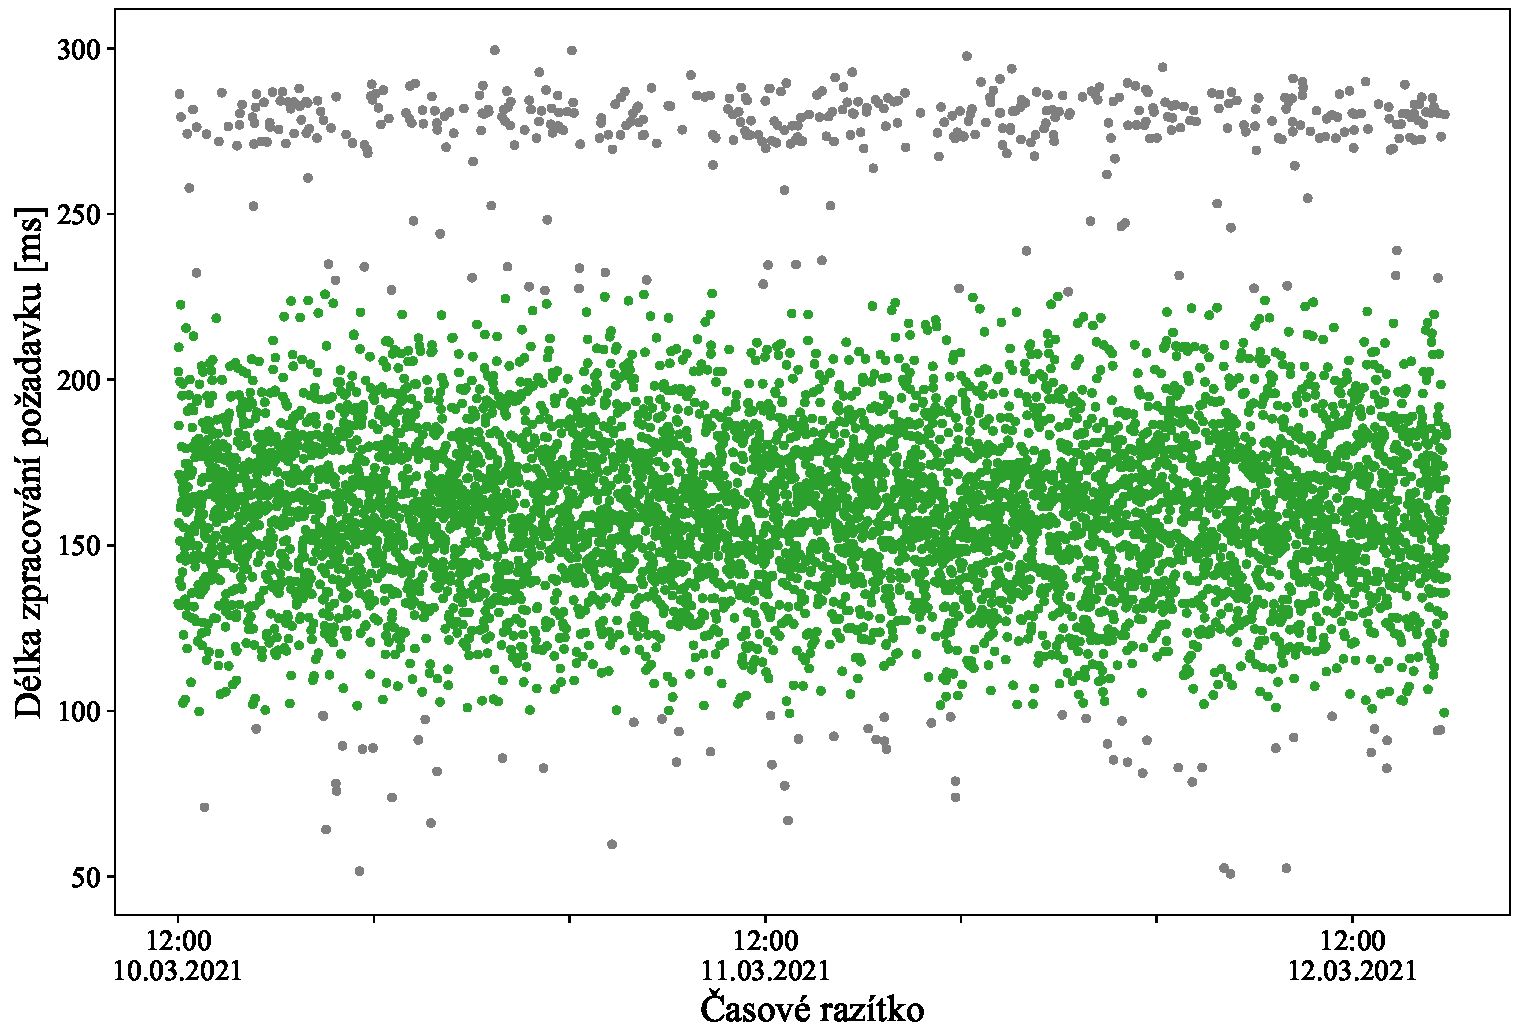
\includegraphics[width=0.935\textwidth]{obrazky/modified-zscore-outlier-detection-success.pdf}
    \caption{Výsledek modifikovaného z-skóre pro detekci outlierů}
    \label{modified-zscore-outlier-detection-success-img}
\end{figure}

\begin{figure}[!hbt]
    \centering
    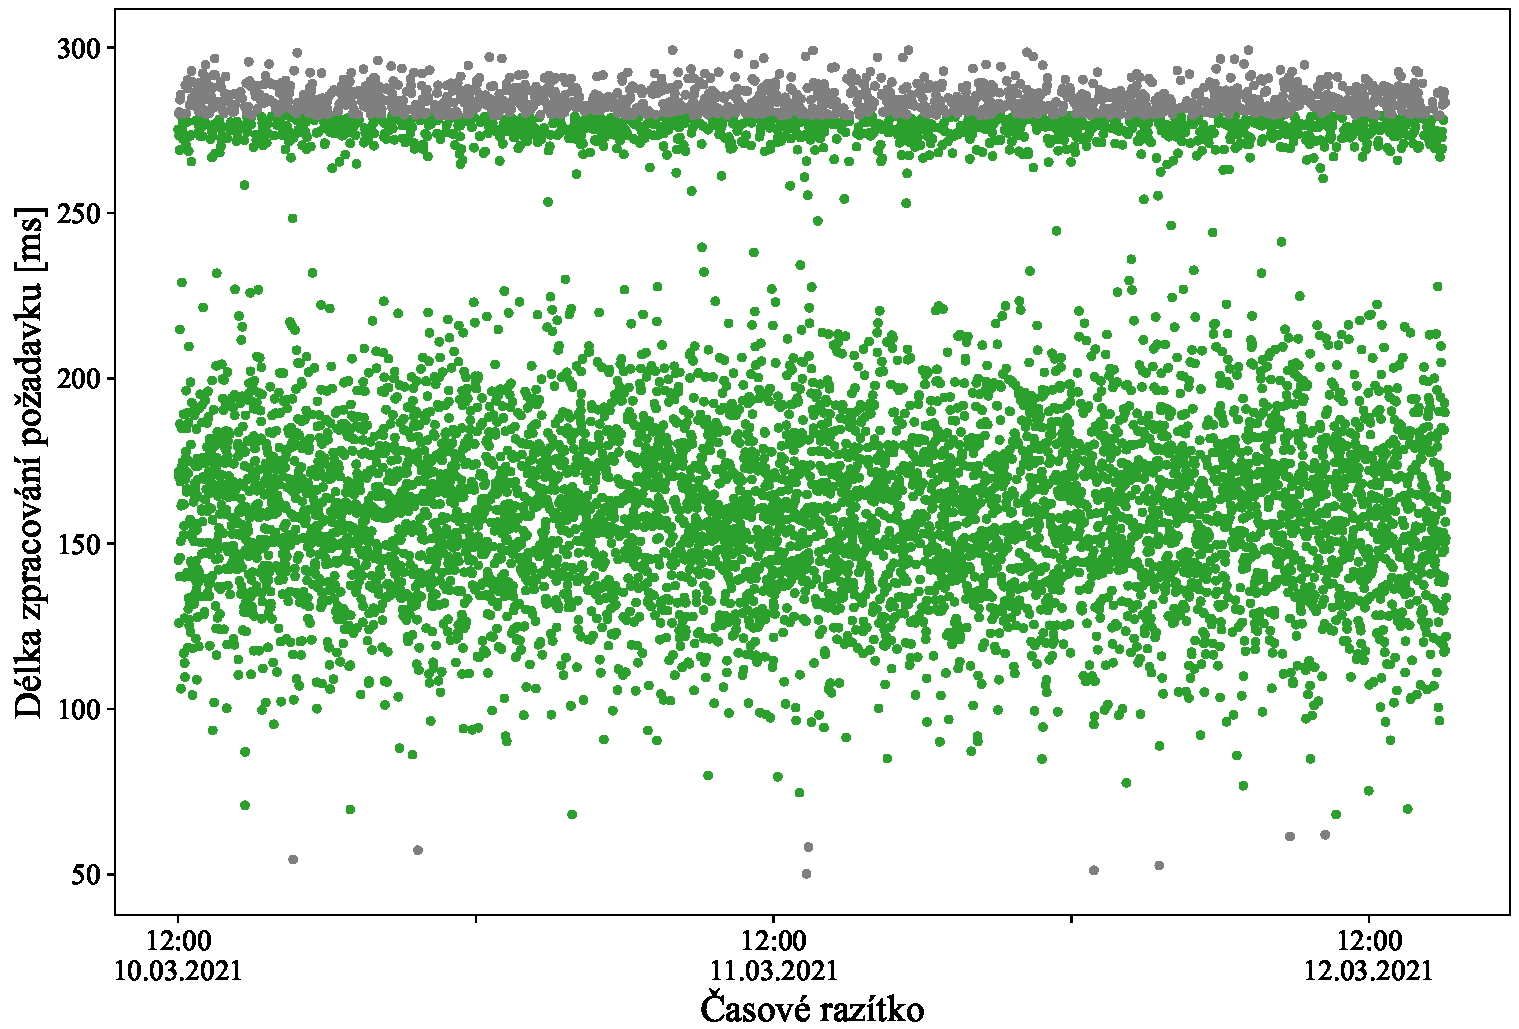
\includegraphics[width=0.935\textwidth]{obrazky/modified-zscore-outlier-detection-fail.pdf}
    \caption{Velká anomálie je schopna posunout medián směrem k~ní a zvětšit MAD natolik, že její část může být považována za platnou.}
    \label{modified-zscore-outlier-detection-fail-img}
\end{figure}

Žádný z~kandidátních algoritmů samostatně nedosahuje optimálních výsledků. Lze však použít jejich kombinaci, konkrétně tedy modifikované z-skóre a DBSCAN. Odstranit problém z~obrázku~\ref{modified-zscore-outlier-detection-fail-img} je možné pomocí parametrů neovlivněných anomálií. V~případě již existujícího referenčního datasetu lze aplikovat samotné modifikované z-skóre. Referenční dataset určuje, kde se nachází platná data, tedy správné centrum v~novém datasetu. Medián a MAD se proto vypočítají z~referenčního datasetu a tyto parametry modifikované z-skóre použije na~nově příchozí data. Referenční dataset se však nejprve musí vytvořit, a~proto je nutné mít způsob nalezení korektního centra datasetu i bez něj. Zde přichází na~řadu DBSCAN. Jak již bylo ukázáno, přestože není moc přesný u~krajních hodnot, hlavní shluk nebo-li hledané centrum datasetu nalézá spolehlivě. Výsledným řešením je tedy nalézt hlavní shluk pomocí DBSCANu, z~něj vypočítat medián a MAD a s~těmito parametry aplikovat modifikované z-skóre na~celý dataset. Tento proces je ukázán na~obrázku~\ref{final-outlier-detection-img}. Modifikované z-skóre rozšíří hlavní shluk nalezený algoritmem DBSCAN, čímž vylepší klasifikaci krajních hodnot. Samo pak díky právě DBSCANu nebude nikdy ovlivněno žádnou anomálií.

\begin{figure}[!hbt]
    \centering
    \subfloat[\centering Nalezení hlavního shluku algoritmem DBSCAN]
    {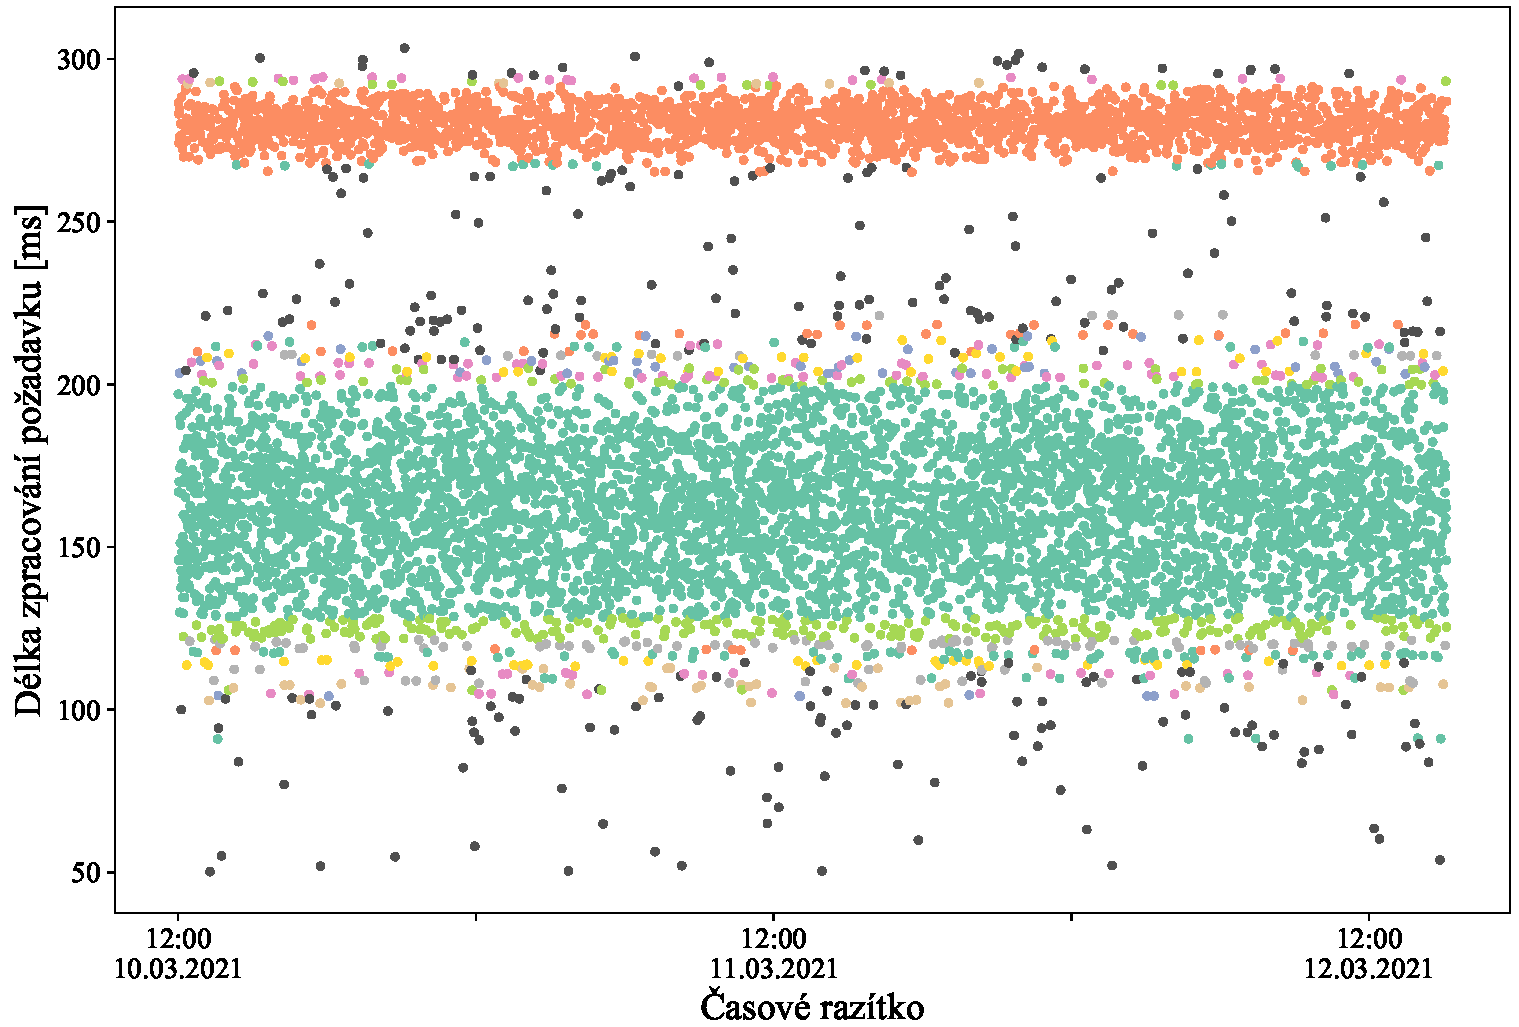
\includegraphics[width=0.935\textwidth]{obrazky/outlier-detection-dbscan-step.pdf}}
    \qquad
    \subfloat[\centering Výsledek modifikovaného z-skóre s~parametry nalezeného hlavního shluku]
    {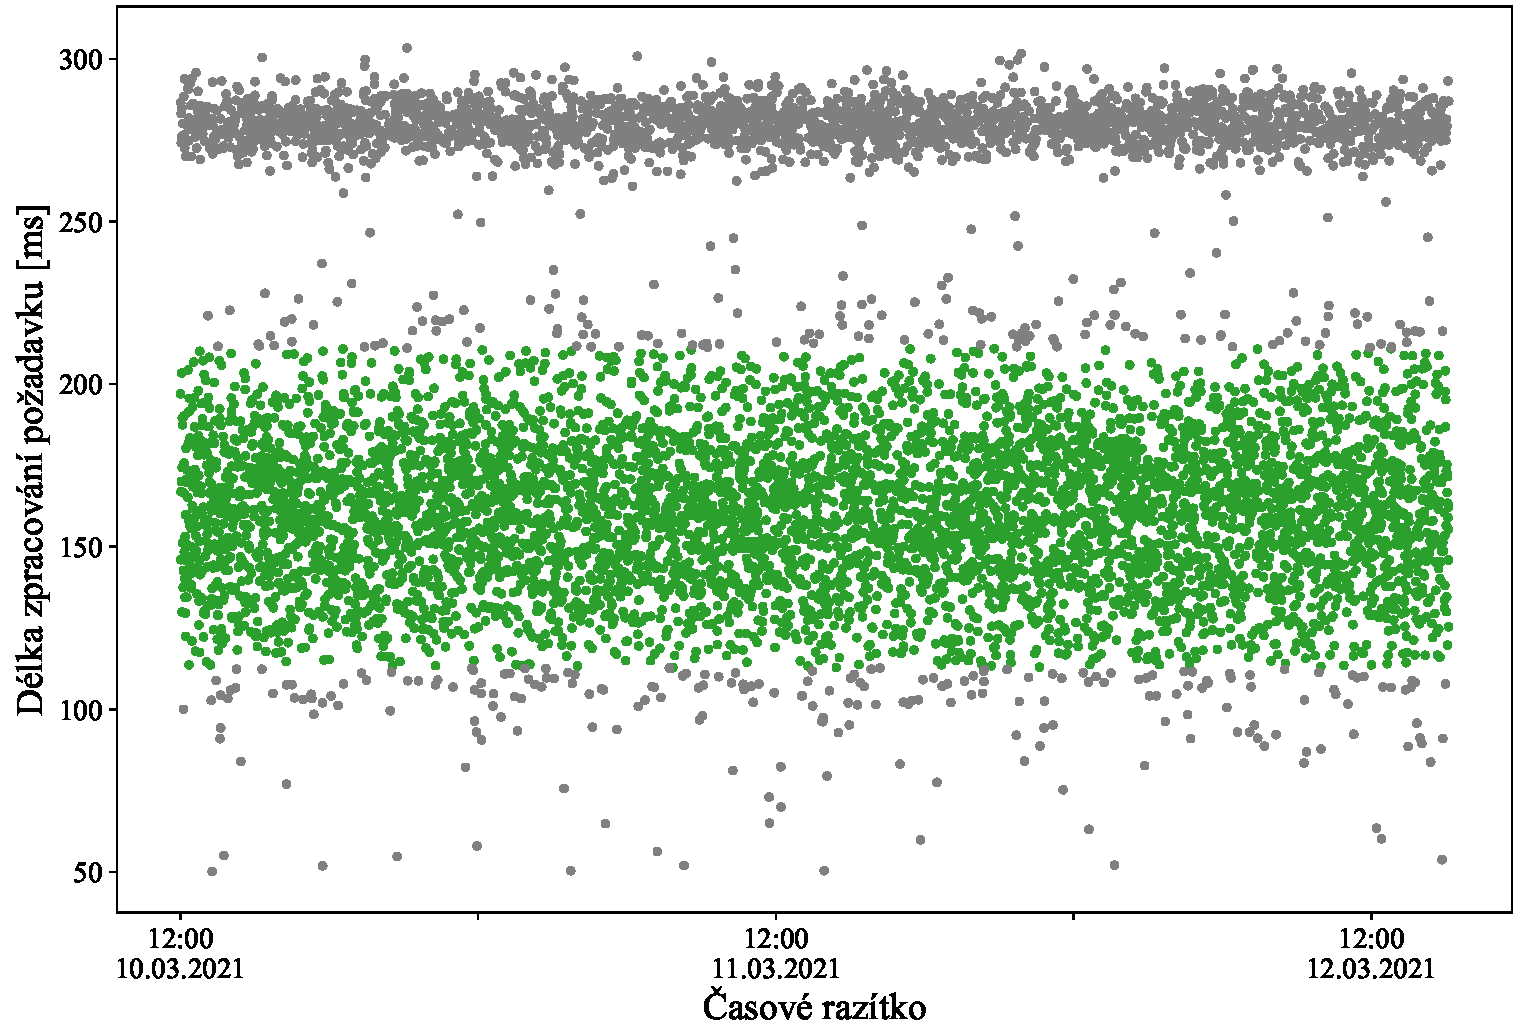
\includegraphics[width=0.935\textwidth]{obrazky/outlier-detection-zscore-step.pdf}}
    \caption{Výsledný postup detekce outlierů kombinací algoritmu DBSCAN a modifikovaného z-skóre}
    \label{final-outlier-detection-img}
\end{figure}

\subsection{Shluková analýza nad outliery}
K~nalezení shluků mezi outliery je možné opět použít HDBSCAN či OPTICS. Nyní je již v~porovnání s~postupem v~sekci~\ref{shlukova-analyza-nad-kolekci-dat} hledání parametrů mnohem jednoduší, neboť nehrozí chybné shlukování platných dat. Z~těchto dvou algoritmů byl vybrán HDBSCAN, neboť je rychlejší, má na~rozdíl od~OPTICS implementaci na~.NET platformě a i hledání parametrů se ukázalo být snazší. Parametr minimální velikosti shluku je poměrně intuitivní. Vzhledem k tomu, že outliery tvoří již značně menší dataset a přebytečné shluky lze jednoduše ignorovat, je lepší mít menší nároky na~shluk. Za~limit proto bylo vybráno alespoň~5~\% z~celkového počtu outlierů. Parametr~\emph{k}, tedy index souseda pro~výpočet vzdálenosti vzájemné dosažitelnosti, zjednodušeně udává hranici mezi šumem a shlukem. Čím vyšší~\emph{k}, tím spíše se bod identifikuje jako šum místo člena shluku~\cite{hdbscan}. Opět protože je shluky spíše žádoucí nalézat, je dobré přiřadit tomuto parametru nižší hodnotu, jíž zpočátku bylo~5~\% z~minimální velikosti shluku. V~průběhu testování se však tato hodnota postupně navýšila až na~10~\%. Vzhledem k~procentuálním výpočtům je nutné určit nepřekročitelná minima těchto parametrů, jimiž jsou~3 pro~minimální velikost shluku a 1 pro~\emph{k}. Na~obrázku~\ref{anomaly-detection-hdbscan-img} je ukázán výsledek HDBSCAN algoritmu nad~outliery.

\begin{figure}[hbt]
    \centering
    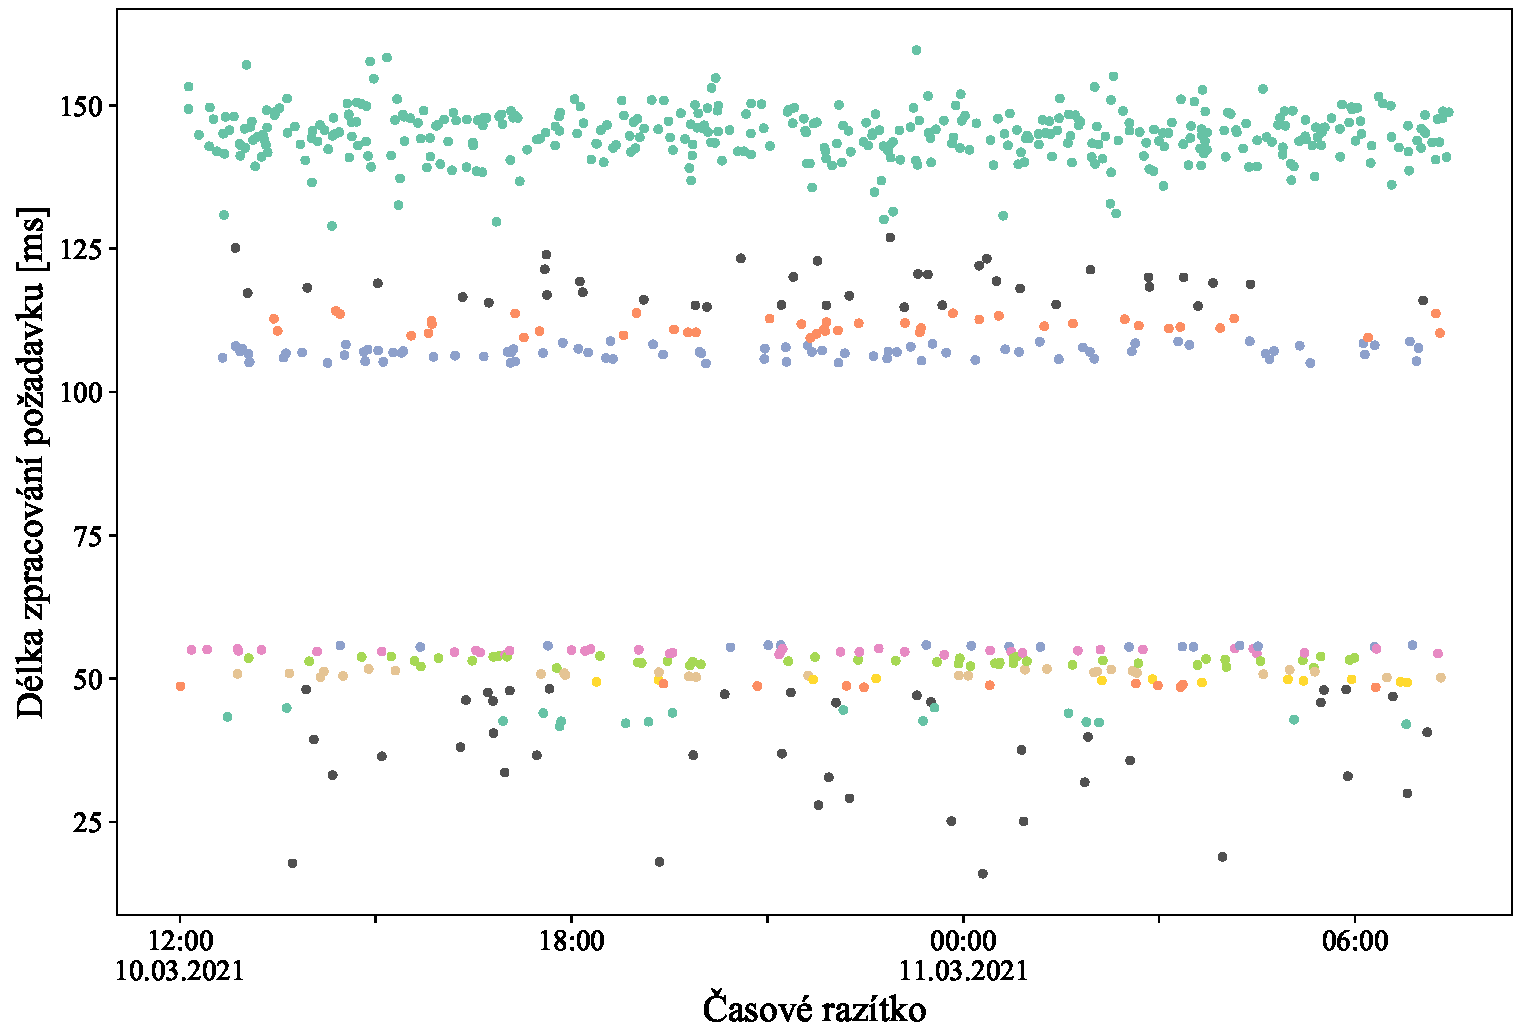
\includegraphics[width=0.88\textwidth]{obrazky/anomaly-detection-hdbscan.pdf}
    \caption{Shluky outlierů nalezené algoritmem HDBSCAN}
    \label{anomaly-detection-hdbscan-img}
\end{figure}

Ukázalo se, že HDBSCAN pracuje poměrně dobře s~ohledem na~obecnost a kvalita výsledků roste s~počtem dat. Na~druhou stranu při~méně než~30 outliery zcela selhává a většinou nenalezne nic. U~takto málo dat ovšem nemá ani cenu řešit různorodost hustot, a~proto lze použít DBSCAN, jenž je dokáže shlukovat kvalitně. Jako MinPts se používá hodnota 3 kvůli co nejmírnějším požadavkům na~shluk. Za~\textepsilon~je volen medián ze~vzdáleností ke~\emph{k}-tému sousedu, kde \emph{k} je polovina z~celkového počtu outlierů. To zajistí relativně velký rozptyl, tedy zvýší šanci na~vytvoření shluku. Jelikož outliery mohou být velmi rozptýleny, je tato vzdálenost shora omezena na~čtvrtinu rozptylu platných dat, aby se nevytvářely příliš široké a řídké shluky.

Navzdory přijatelným výsledkům však nelze nalezené shluky považovat za~konečné. Z~důvodu požadavku na~obecnost detekce jsou tyto podobně jako ty od~DBSCANu v~předchozí sekci jen hrubé. Na~konkrétním příkladu z~obrázku~\ref{anomaly-detection-hdbscan-img} je anomální shluk nalezen celý, nicméně přirozené krajní outliery zde nezobrazených platných dat vytvořily zbytečně mnoho malých shluků, což se v~jiném případě může stát i anomálnímu shluku. V~závislosti na~tvaru a počtu dat budou tyto výsledky vždy jiné, občas zcela přesně rozdělené na~správné shluky, jindy zase až příliš jemně.

Problém příliš malých shluků je řešen sloučením blízkých sousedů. Každý shluk je poměřen s~jeho následujícím sousedem a kontroluje se, zda-li nejsou blízko sebe. Vzájemná blízkost se měří následovně. Překrývají-li se dva shluky s~ohledem na~pravidlo 3-sigma, tedy platí-li nerovnice \(median_1 + 3\sigma_1 > median_2 - 3\sigma_2\), shluky jsou blízké. Během testování se občas ukázaly případy, kdy byl nějaký shluk rozdělen na~mnoho menších shluků příliš úzkých na~sloučení na~základě 3-sigma. Musela se proto zavést i fixní minimální vzdálenost mezi~2 shluky. Idea spočívala v~tom vzít nízké procento rozptylu platných dat, jež se v~průběhu testování ustálilo na hodnotě~2.5~\%. Je-li tedy vzdálenost mezi dvěma shluky menší než~2.5~\% rozptylu platných dat, jsou taktéž blízké.

Druhou podmínkou pro~sloučení je vedle blízkosti i podobná hustota. Z~obou shluků se vezme polovina sousedící s~druhým shlukem, tedy pravá polovina levého shluku a levá polovina pravého shluku. Z~každé se spočítá medián vzdáleností ke~\emph{k}-tému sousedu, kde~\emph{k} je menší z~hodnot 10 a polovina velikosti dané poloviny shluku. Co se zvolí za~hodnotu \emph{k}~není příliš významné, neboť vzdálenost k~dalším sousedům roste s~\emph{k} úměrně díky rovnoměrné hustotě shluku zajištěné algoritmem HDBSCAN. Hodnota~10 byla zvolena proto, že u~vyšších by se již jen zbytečně počítalo více vzdáleností a naopak nízké jednotky by přece jen mohly trpět lokálními výkyvy. Tato vzdálenost ke~\emph{k}-tému sousedu tak udává jistou míru hustoty a je-li jedna více než 2.5krát větší než druhá, tedy jeden shluk je výrazně hustší než druhý, není splněna podmínka podobné hustoty. Hodnota~2.5 byla zvolena na~základě porovnání různých hustot rovnoměrných rozložení jako zobrazuje obrázek~\ref{porovnani-hustot-img}. Dvojnásobná hustota ještě poměrně splývá, trojnásobná již však vyčnívá příliš. Hodnota~2.5 se ukázala být dobrou kompromisní hranicí. Ve~výsledku se sloučí pouze ty sousední shluky, které jsou blízko sebe a mají podobnou hustotu. Celý proces se iterativně opakuje, dokud existují slučitelné shluky. Obrázek~\ref{anomaly-detection-merged-clusters-img} zobrazuje výsledek celého procesu shlukování outlierů.

\begin{figure}[!hbt]
    \centering
    \subfloat[\centering 2x větší hustota]{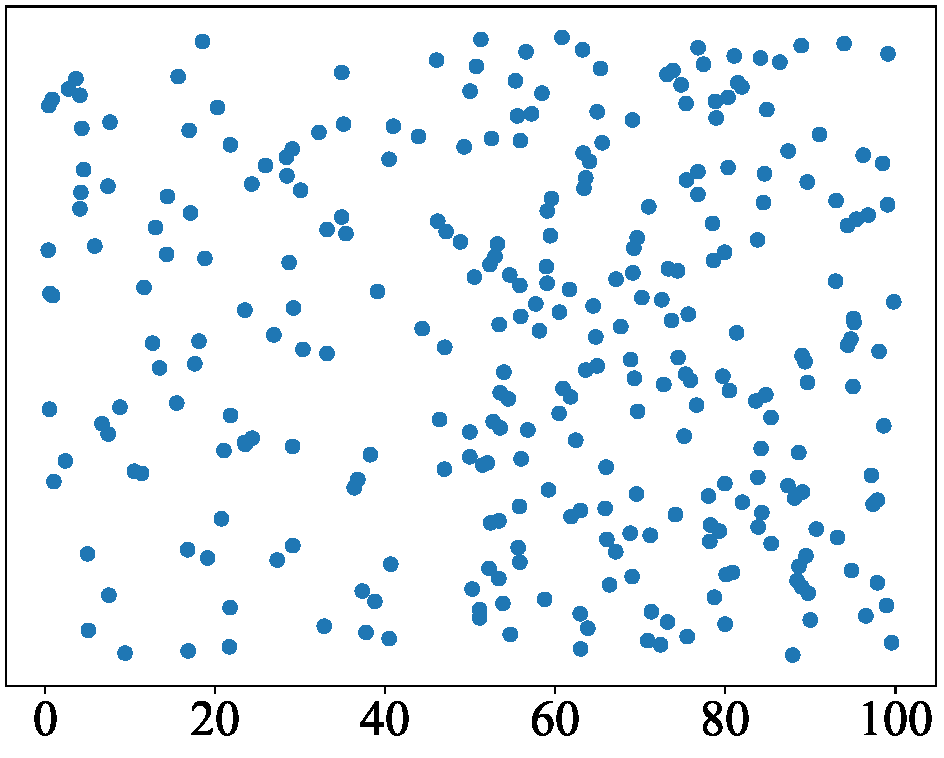
\includegraphics[width=0.32\textwidth]{obrazky/density-2x.pdf} }
    \subfloat[\centering 2.5x větší hustota]{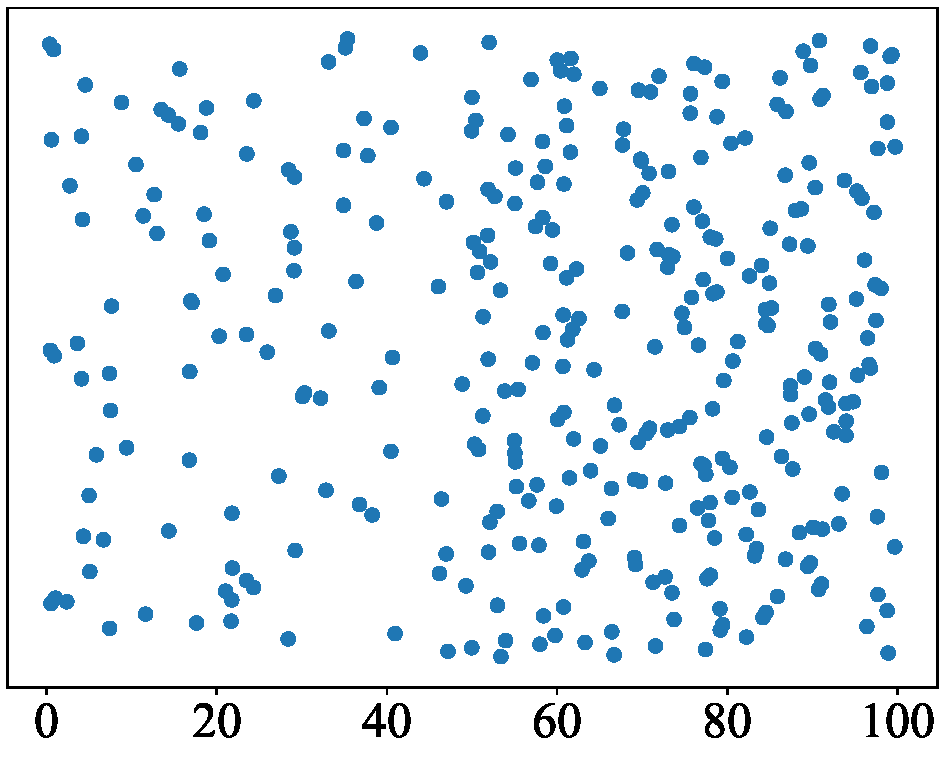
\includegraphics[width=0.32\textwidth]{obrazky/density-2.5x.pdf} }
    \subfloat[\centering 3x větší hustota]{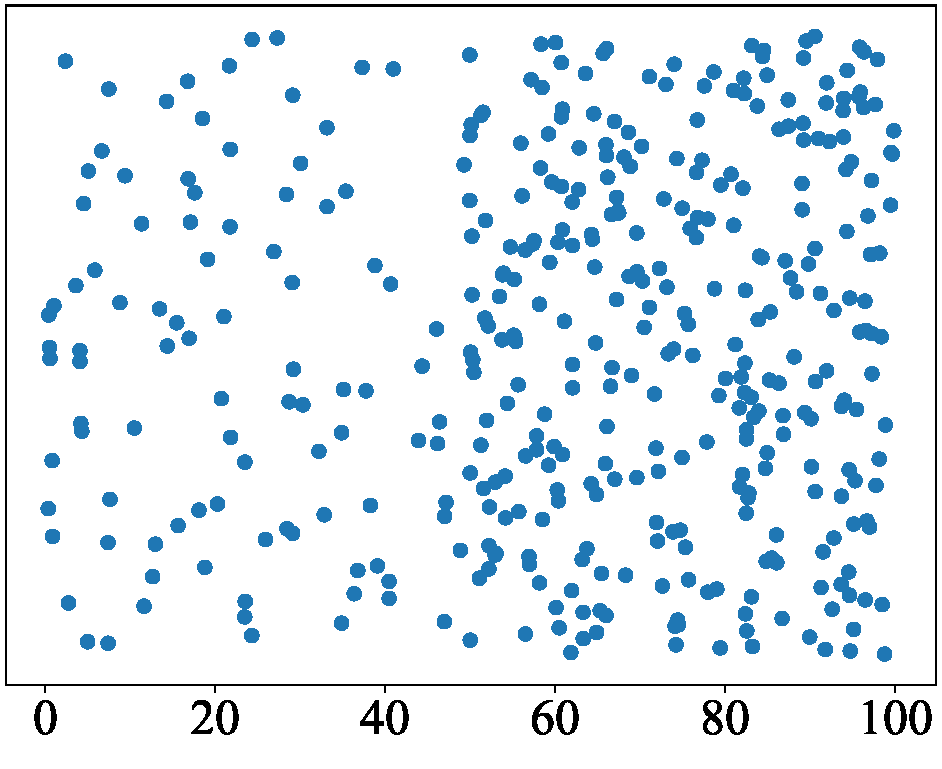
\includegraphics[width=0.32\textwidth]{obrazky/density-3x.pdf} }
    \caption{Porovnání rozložení s~odlišnou hustotou. V~intervalu 0-50 je porovnávané rozložení, mezi 50-100 jsou vždy hustší rozložení.}
    \label{porovnani-hustot-img}
\end{figure}

\begin{figure}[!hbt]
    \centering
    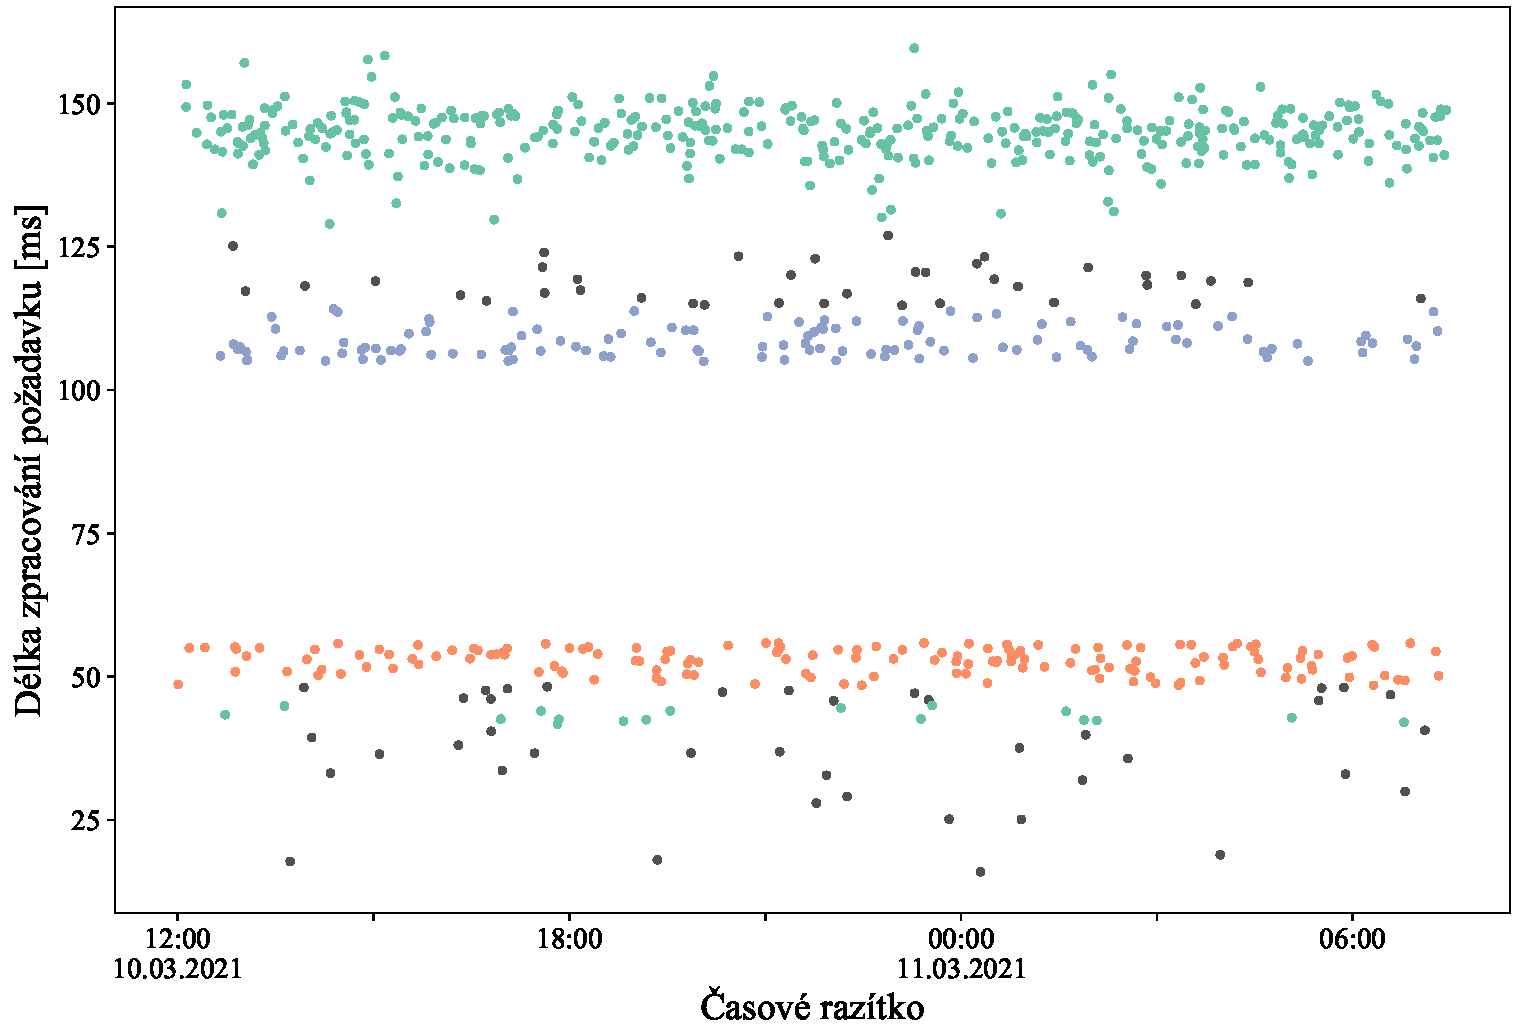
\includegraphics[width=0.84\textwidth]{obrazky/anomaly-detection-merged-clusters.pdf}
    \caption{Výsledek shlukování outlierů po~sloučení blízkých shluků}
    \label{anomaly-detection-merged-clusters-img}
\end{figure}

\subsection{Rozpoznání anomálie mezi shluky outlierů}
Anomálie byla dříve v~práci definována jako shluk outlierů, nicméně prohlásit všechny čtyři shluky z~obrázku~\ref{anomaly-detection-merged-clusters-img} za~anomálie by bylo mylné. Hlavním kritériem pro anomálii je velikost shluku. Shluk je považován za~anomálii, jestliže je větší než určitá mez. Touto je~5~\% celkové velikosti datasetu. Jedná se však o~uživatelsky nastavitelnou hodnotu, neboť udává pouze anomální toleranci a nemá žádný vliv na~samotný výpočet. Nicméně, před kontrolou velikosti shluků je ještě potřeba provést několik úkonů.

Je zcela patrné, že fialový a oranžový shluk z~obrázku~\ref{anomaly-detection-merged-clusters-img} obsahují krajní hodnoty platných dat, které již byly klasifikovány jako outliery. Tyto budou dále označovány jako \uv{přirozené outliery}. Přestože přirozené outliery tvoří shluky a často dostatečně velké na~to, aby byly považovány za~anomálie, o~anomálie se nejedná. Je proto potřeba tyto umět rozpoznat. Každý nalezený shluk je tedy podroben následujícímu testu. Pokud sousedí s~platnými daty, je jim dostatečně blízko a má řídnoucí tendenci, nebo-li počet jeho prvků ubývá se vzdáleností od~platných dat, jedná se o~přirozené outliery a shluk není prohlášen za~anomálii.

Blízkost se sousedstvím se zjistí tak, že se pro~každý prvek shluku vypočítá medián jeho vzdáleností od~ostatních prvků a jako sousedská vzdálenost se použije jejich medián. Dále existuje-li nějaký platný prvek v~této vzdálenosti od~shluku, lze shluk prohlásit za~souseda platných dat. Ověření řídnoucí tendence probíhá ve~dvou krocích. Nejprve se porovná velikost shluku se~stejně širokou oblastí platných dat. Pokud by byl shluk výrazně větší, tak i kdyby jeho prvky řídly v~rámci něj, neřídnou v~porovnání s~platnými daty. Tolerance je nastavena tak, že shluk může být až~2.5krát větší než stejně široká oblast platných dat. Tato volnost je z~toho důvodu, že rozložení zejména menších datasetů nemusí být pravidelné a na~straně platných dat zrovna může být lokální pokles, který však nic neznamená. Ke~konkrétní hodnotě~2.5 se dospělo během testování při~snaze minimalizovat falešné detekce přirozených outlierů za~anomálie. Druhým krokem je test řídnutí v~rámci shluku samotného. Ten se provádí pouze, pokud je shluk dostatečně velký, konkrétně pokud obsahuje alespoň~15 prvků, jinak nelze tuto vlastnost s~dostatečnou jistotou určit. Test používá metodu modifikovaného z-skóre, která každému prvku přiřadí anomální skóre. Vzhledem k~tomu, že je požadováno, aby blíže k~platným datům byl shluk hustší, prvky na~tomto okraji by měly mít nižší skóre, zatímco na~druhém vyšší. Během práce bylo experimentálně zjištěno, že krajní hodnoty rovnoměrného rozložení mají modifikované z-skóre v~rozmezí~1.3 až~1.4. Z~důvodu možnosti mírných výkyvů se tolerance nastavila na hodnotu~1.7. Ve výsledku tedy pokud má krajní hodnota shluku blíže k~platným datům modifikované z-skóre nižší než~1.7, shluk má řídnoucí tendenci, nebo má přijatelné výchylky. Jestliže je toto skóre vyšší, má buď výrazný výkyv, nebo jeho prvky houstnou.

Dalším úkonem před kontrolou velikosti shluků na anomálie je vyhlazení shluků. Anomální horní zelený shluk na~obrázku~\ref{anomaly-detection-merged-clusters-img} obsahuje i několik okolních outlierů, které by již nemusely být jeho součástí. Shluk lze aplikováním modifikovaného z-skóre vyhladit a tím zpřesnit. Princip však funguje i obráceně. Pokud by shlukování nalezlo pouze střed shluku a krajní hodnoty by vynechalo, modifikované z-skóre by shluk rozšířilo alespoň o~část krajních hodnot. V~obou případech modifikované z-skóre opraví a vylepší shluk. V~první řadě je potřeba zjistit, zda-li je žádoucí shluk rozšířit či zúžit. Myšlenka spočívá v~tom, že pokud má shluk výraznou špičku, již zřejmě nepotřebuje rozšíření. Většina dat je totiž ve~špičce, zatímco na~jejích krajích data řídnou a nelze předpokládat další data ve~významném množství. Naopak je-li shluk rovnoměrnější s~pouze mírnou špičkou, zřejmě lze za~hranicemi shluku nalézt další data, jež jsou krajními prvky rozložení shluku.

Prakticky se to provede aplikováním modifikovaného z-skóre na~shluk stejným způsobem jako u~detekce outlierů popsané v~podkapitole~\ref{detekce-outlier}, tedy s~mediánem a mediánem absolutní odchylky daného shluku a hraničním skóre~2.35. Jsou-li nalezeny nějaké outliery nebo je průměr skóre nejlevějšího a nejpravějšího prvku větší než~1.45, tedy přesahující krajní hodnoty rovnoměrného rozložení, ve~shluku je špička, a~proto se bude vyhlazovat. V~opačném případě se shluk bude rozšiřovat. Při~vyhlazování se jako nový shluk použijí pouze platná data shluku po~výše použitém modifikovaném z-skóre. V~případě rozšiřování se shlukem stane výsledek modifikovaného z-skóre s~parametry daného shluku aplikovaném na všechny outliery. Protože shluk je úzký a cílem je ho rozšířit, musí se zvýšit i limit hraničního skóre.
Uvažovalo by-li se, že takovýto zúžený shluk má šířku polovinu normálního rozložení, tedy~1.5 sigma, na~rozptyl daný skórem 2.35 u~plného rozložení by se dosáhlo hodnotou skóre cca~2.9. Během testování dle sekce~\ref{testovani-konkretni-anomalie} se toto upravilo na~hodnotu~2.95.

Po~odstranění shluků s~přirozenými outliery a korekcí zbývajících shluků již zbývá jen porovnat velikost shluků s~anomálním limitem. Pokud je shluk dostatečně velký, jedná se o~anomálii. Obrázek~\ref{anomaly-detection-anomalous-cluster-img} zobrazuje výsledek rozpoznání anomálních shluků a ve~srovnání s~obrázkem~\ref{anomaly-detection-merged-clusters-img} na~něm lze i vidět vyhlazení anomálního shluku. Obrázek~\ref{anomaly-detection-histogram-img} pak formou histogramu znázorňuje celkový výsledek detekce anomálií.

\begin{figure}[hbt]
    \centering
    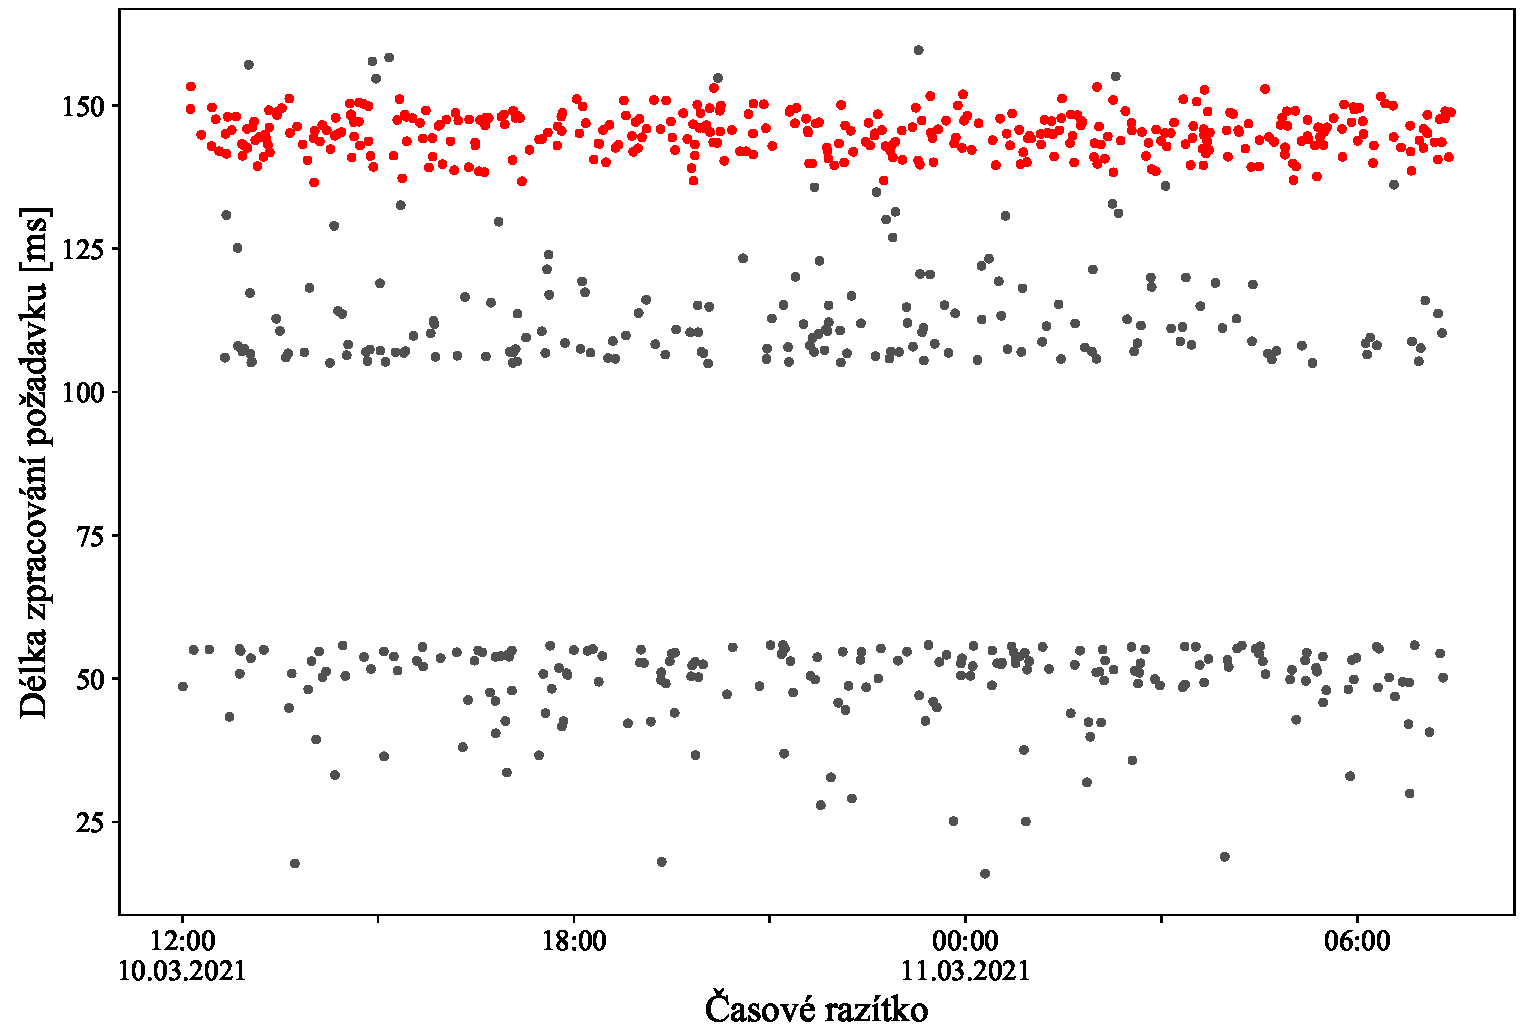
\includegraphics[width=0.935\textwidth]{obrazky/anomaly-detection-anomalous-cluster.pdf}
    \caption{Nalezený anomální shluk mezi shluky outlierů}
    \label{anomaly-detection-anomalous-cluster-img}
\end{figure}

\begin{figure}[!hbt]
    \centering
    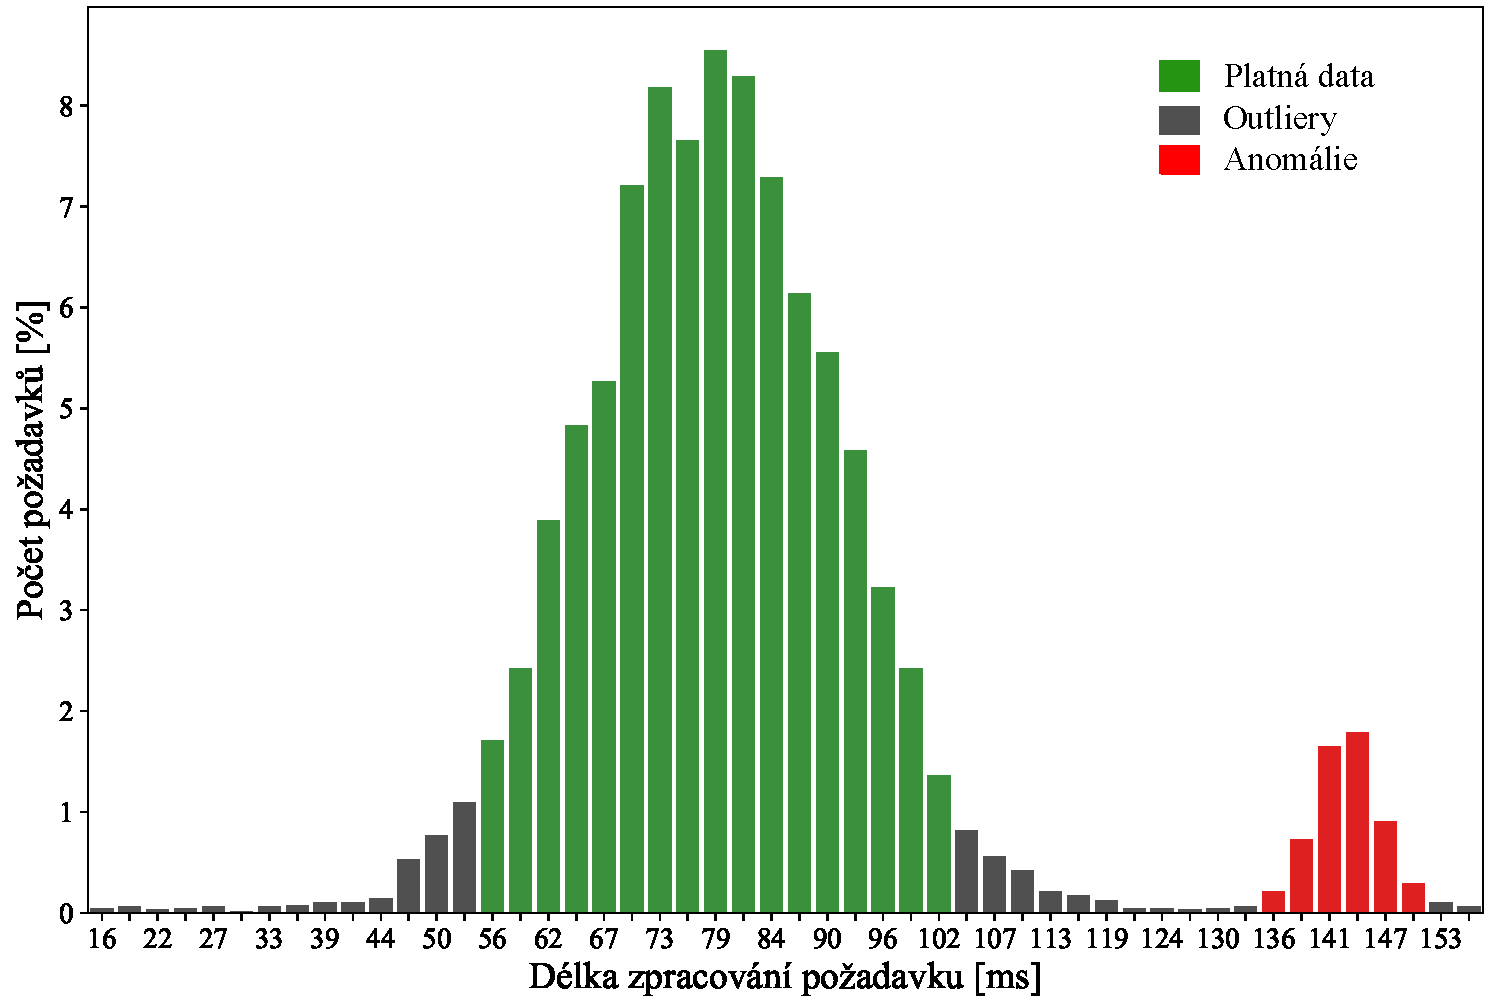
\includegraphics[width=0.935\textwidth]{obrazky/anomaly-detection-histogram.pdf}
    \caption{Celkový výsledek detekce anomálií}
    \label{anomaly-detection-histogram-img}
\end{figure}

Při~práci s~reálnými daty v~RQA systému se ukázalo, že občas je rozptyl délek zpracování požadavků velmi malý, třeba v~jednotkách nebo i zlomcích milisekund. V~tomto případě se i shluk vzdálený jen pár milisekund detekuje jako anomální, neboť relativně ke~zbytku je velmi daleko. Reálně se však jedná skutečně jen o~několik milisekund, což je velmi často zanedbatelné, a~proto může být výhodné umět takové anomálie potlačit. Z~toho důvodu byl zaveden volitelný parametr tolerance, jenž udává, v~jaké vzdálenosti od~platných dat nebudou anomálie detekovány. Prakticky to pouze znamená, že pokud by se měl shluk prohlásit za~anomálii, tak se ještě zkontroluje jeho vzdálenost od~platných dat a jestli je tato menší než daná tolerance, anomálií se nestane.

\section{Detekce anomálií v~chybovosti požadavků}
\label{detekce-anomálii-v-chybach}
Počet chyb během požadavků typicky nabývá hodnoty 0, pokud vše proběhlo v~pořádku, nebo 1 v~případě fatální chyby, která ukončí vykonávání požadavku. Jiné hodnoty se vyskytují pouze u~takových požadavků, které se z~chyb dokáží vzpamatovat. Příkladem může být úspěšná klasifikace obrázku až na~několikátý pokus nebo změna chodu programu po~chybě namísto ukončení.

Hodnoty, s~nimiž se pracuje, jsou tedy celočíselné v~rozmezí 0-N, kde N jsou nízké jednotky. Na~taková data nemá význam shlukování vůbec aplikovat. Místo toho lze použít statistiku, která je mnohem jednodušším i rychlejším řešením. V~podstatě stačí spočítat a porovnat poměry množství chyb v~referenčním datasetu a v~nově příchozích datech. Každá hodnota má nějaké procentuální zastoupení a jestli se toto liší o~více než zvolenou mez, kterou je ve výchozím nastavení hodnota 10~\%, lze to považovat za~anomálii. Podobně je anomálií taková situace, kdy se u~nějakého požadavku vyskytne doposud neviděný počet chyb.

\section{Implementace detekce anomálií}
\label{implementace-detekce-anomalii}
Sekce~\ref{zpracovani-a-ulozeni-dat} zmínila nějakou aplikaci provádějící detekci anomálií. V~sekci~\ref{implementace-sberu-dat} bylo dále uvedeno, že je sběr dat implementován jako knihovna, nikoliv jako specifická spustitelná aplikace. Stejným způsobem je řešena i samotná detekce. Výstupem této práce jsou tedy knihovny použitelné libovolným způsobem. Může tak existovat jedna aplikace, která obstarává sběr dat i detekci, nebo tyto mohou být oddělené. 

Očekávaným vstupem pro~knihovnu jsou buď CSV soubory nebo datové struktury s~již načtenými daty. Knihovna poté data roztřídí na~platné vzory, outliery a anomálie v~případě délek zpracování požadavků nebo u~chybový požadavků pouze určí, zda se jedná o~anomální stav. Knihovna umí i generovat XPlot grafy pro~vizuální zobrazení výsledků.

Detekci anomálií implementuje projekt \emph{AnomalyDetection.Application}, jak již sekce~\ref{implementace-sberu-dat} taktéž naznačila. Není však zcela samostatný a odkazuje na~\emph{AnomalyDetection.Data}, neboť využívá některé jeho třídy. Na~následujícím obrázku~\ref{diagram-zavislosti-trid} je zobrazen diagram závislostí předních tříd podílejících se na detekci anomálií. Neobsahuje pomocné modelové třídy.

\begin{figure}[hbt]
    \centering
    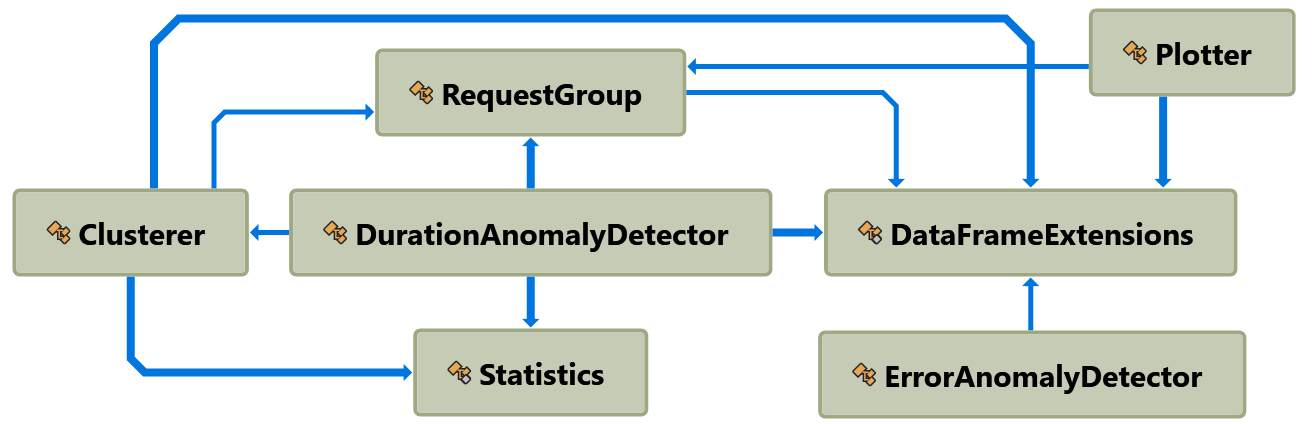
\includegraphics[width=1\textwidth]{obrazky/anomaly-detection-class-dependency-diagram.png}
    \caption{Diagram závislostí tříd ústředních pro~detekci anomálií}
    \label{diagram-zavislosti-trid}
\end{figure}

Analyzovaná data jsou interně reprezentována pomocí dataframů poskytovanými knihovnou \emph{Microsoft.Data.Analysis}. Práce s~nimi ovšem není tak příjemná jako například s~těmi knihovny \emph{Pandas} jazyka Python, a~proto v~projektu existuje třída \texttt{DataFrameExtensions} implementující rozšíření pro~lepší manipulaci s~nimi. Jako kontejner pro~dataframy slouží třída \texttt{RequestGroup}, která zastřešuje všechna data napříč celé analýzy pro~daný typ požadavku určité služby. Obsahuje dataframe zvlášť pro~platná data, outliery, anomálie nebo i mezikroky detekce. Tato data lze vizualizovat pomocí třídy \texttt{Plotter}.

Velký význam pro~detekci anomálií mají statistické výpočty, o~které se stará třída \texttt{Statistics}. Obsahuje metody pro~výpočet modifikovaného z-skóre, mediánu absolutní odchylky, mediánů vzdáleností mezi sousedy nebo i pro generování náhodných čísel.

Další ústřední třídou je \texttt{Clusterer}. Ta implementuje veškeré operace spojené se~shlukováním. Především se jedná o~aplikaci algoritmů DBSCAN a HDBSCAN dostupných z~knihoven \emph{DBSCAN.RBush} a \emph{HdbscanSharp}. Zde stojí za~zmínění, že tato HDBSCAN implementace je v~době psaní práce v~.NET jediná a má značný nedostatek. Vzájemné vzdálenosti bodů jednoduše uchovává ve~2D~poli, oproti například právě DBSCANu, jenž využívá RBush strom. Tím pádem má kvadratickou paměťovou složitost, a nedokáže proto zpracovat velké množství dat. Například dataset o~50 000 prvcích by vyžadoval~\(50 000\times50 000\times8 = 20\)~GB paměti. Dodatečných \(\times8\) proto, že se jedná o~typ \texttt{double}, jenž má velikost 8~B. Naštěstí se HDBSCAN aplikuje pouze na~outliery, které by nikdy neměly dosahovat z~tohoto pohledu nebezpečného množství. Detekce anomálií se totiž bude provádět dostatečně často, aby tak velké datasety ani nevznikaly.

Dále \texttt{Clusterer} obsahuje metody pro~normalizaci výsledků těchto algoritmů. Žádoucí je mít pro~každý bod číselné označení shluku, ke~kterému patří. DBSCAN však vrací kolekci seznamů, kde každý seznam reprezentuje shluk. Výsledek HDBSCANu pak sice je seznam číselných označení pro~každý bod, nicméně tyto nejsou rozumně seřazeny od~nuly, nýbrž se jedná o~čísla uzlů v~kondenzovaném stromu. Po normalizaci mají šumové body přiřazenu hodnotu -1 a ostatní dle příslušnosti ke~shluku 0-N, kde N je počet shluků.

Náročnější na~implementaci se ukázalo být slučování blízkých shluků. Nejprve je nutné seřadit shluky dle hodnot mediánů, aby bylo možné porovnat přímé sousedy. Poté se mezi všemi sousedy otestuje podmínka na slučitelnost, čímž vzniknou dvojice indexů shluků ke~sloučení. Následně se sloučí ty dvojice, které mezi sebou mají tranzitivní vztah, výsledkem čehož jsou seznamy indexů shluků tvořící výsledné shluky. V~posledním kroku se shluky sloučí dle těchto seznamů. V~neposlední řadě \texttt{Clusterer} implementuje kontrolu shluku na~přirozené outliery platných dat.

Za~řízení detekce anomálií mezi délkami zpracování požadavků nese odpovědnost třída \texttt{DurationAnomalyDetector}. Ta ve svém veřejném protokolu zpřístupňuje pouze metody \texttt{FindOutliers()} a \texttt{FindAnomalies()}, které se řídí návrhem z~kapitoly~\ref{detekce-anomalii-v-delkach-pozadavku} a pro~dílčí operace využívají třídy \texttt{Statistics} a \texttt{Clusterer}. Třída \texttt{ErrorAnomalyDetector} pak zase obstarává detekci anomálií v~chybovosti požadavků. Jedná se o~malou třídu s~jedinou metodou \texttt{IsInputAnomalous()}, jež porovnává poměry počtů chyb mezi vstupními a referenčními daty dle sekce \ref{detekce-anomálii-v-chybach} a vrací výsledek typu \texttt{bool}. 

\section{Čištění kolekce dat}
\label{cisteni-kolekce-dat}
Vlastnoruční generování dat přináší několik výhod, jež usnadňují jejich zpracování. Je zaručeno, že žádné hodnoty nebudou chybět. Všechny hodnoty budou správných typů. Neexistují neplatné hodnoty. Vhodný formát potom zaručuje proces popsaný v~kapitole~\ref{sber-dat}. Jediná věc, která se ještě musí zajistit, je odstranění outlierů z~referenčního datasetu. Řešením je provedení navržené detekce outlierů nad~referenčním datasetem. V~datasetu zůstanou pouze platná data a během dalších detekcí se již tato mohou použít pro~určení outlierů.

Během průběžné detekce v~nových datech se pak do~referenčního datasetu budou přidávat opět pouze platná data a ostatní se zahodí. Toto však platí jen pro~detekci mezi délkami zpracování požadavků. U~počtů chyb se budou přidávat i anomální data, neboť tam se pouze ví, že v~daném detekčním okně byla odlišná chybovost, neznají se konkrétní anomální záznamy. To ve~své podstatě ani není možné, pokud se nevyskytne zcela nová chybová třída. Přidávat anomální chybová data však vůbec nevadí. Jedná se totiž o~určitý přirozený vývoj dat. Navíc existuje korelace mezi počtem chyb a délkou zpracování požadavku. Například fatální chyba způsobí, že požadavek bude trvat kratší dobu. Proto je možné, že se zároveň detekují obě anomálie, chybové záznamy patřící i do~anomálie v~délkách zpracování požadavků se nepřidají a tím se poměr chybovosti opět trochu dorovná.
  \chapter{Testování a vyhodnocení výsledků}
\label{testovani-a-vyhodnoceni}

Oproti učení s~učitelem, kde je trénován model, jemuž často bývá přiřazena procentuální úspěšnost správného rozpoznávání díky anotovaným datům, učení bez učitele žádné takové měřítko neudává. Výsledek není s~čím porovnat, a~proto není možné jasně a číselně validovat výstup. Úkol dále ztěžuje objektivita pohledu na~to, co vůbec anomálií je. Ve~výsledku je tedy nutné, aby každý případ posoudil člověk a vyhodnotil, zda detekce proběhla v~pořádku. Jednotlivé sekce této kapitoly popisují, jak se řešení detekce anomálií testovalo a jaké závěry z~toho vyplynuly.

\section{Testování detekce anomálií v~délkách zpracování požadavků}
\label{testovani-delka-pozadavku}
Aby bylo možné testovat odhalení co nejvíce typů anomálií, bylo potřeba vytvořit dataset odpovídající reálným datům. V~něm pak šlo anomálie vytvářet a ověřovat, zda-li budou detekovány. Prvním způsobem testování bylo vytváření konkrétních dat a anomálií s~cílem vyzkoušení detekce anomálií nad~jejich různými typy. Druhým pak bylo náhodné generování provozu s~anomáliemi, jež se měly odhalovat.

\subsection{Vytvoření a nalezení konkrétní anomálie}
\label{testovani-konkretni-anomalie}
Smyslem tohoto testování bylo ověření schopnosti detekovat co nejvíce typů anomálií. Umožňovalo cíleně vytvářet anomálie různých velikostí, hustot či tvarů. Právě tento způsob testování nejvíce přispěl k~nalezení co nejobecnějších parametrů detekčních algoritmů. Odhaloval jak pozitiva, tak nedostatky hodnot určitých parametrů pro~jeden či druhý typ anomálie, což vedlo ke~kvalitnímu kompromisu.

Dataset se vytvářel následujícím způsobem. Platná data se vždy vygenerovala z~normálního, Fisher-Snedecorova nebo trojúhelníkového rozložení s~parametry odpovídajícími účelům konkrétního testu. Z~rovnoměrného rozložení přesahujícího hranice platných dat se následně vygenerovaly náhodné outliery. Anomálie se poté vytvářely na místech, kde se chtělo otestovat, jestli se tam naleznou. Testovaly se případy, kdy anomálie byly:

\begin{itemize}
  \item velikostí na~hranici limitu nebo naopak skoro stejně velké jako platná data,
  \item různé hustoty a tedy rozptylu, ať už velmi úzké nebo široké,
  \item odlišných rozložení (rovnoměrné, normální, Fisher-Snedecorovo, trojúhelníkové) různých parametrů,
  \item blízko platných dat nebo s~odstupem,
  \item větších počtů, kde se pak všechny vyskytovaly na~stejné straně od~platných dat, z~obou stran, nebo se anomálie navzájem i překrývaly.
\end{itemize}

Chyby nalezené během tohoto testování vedly na~úpravy parametrů detekčních algoritmů. Bylo proto prováděno, dokud se vyskytovaly chyby v~detekci, jež bylo možné odstranit. Testování dovedlo detekci do~stavu, ve~kterém je schopna rozpoznat téměř každou anomálii vytvořenou tímto způsobem. Neodstranitelným nedostatkem nalezeným tímto testováním se ukázala být občasná mylná klasifikace přirozených outlierů jako anomálie. Tento problém však nenastává při použití parametru tolerance anomálií v~určité vzdálenosti od~platných dat.

\subsection{Generování náhodného provozu}
Výše zmíněné testování by šlo zpochybnit tím, že se anomálie úspěšně detekovaly proto, že byly vytvářeny vlastnoručně. Z~toho důvodu a taktéž pro~testování ve~větším měřítku se detekce ověřovala i na~náhodných datech. Ta byla generována podobně jako u~předchozího přístupu a ze~stejných rozložení, neboť tak data v~RQA vypadají. Náhodnost spočívala ve~velikosti, tvaru a pozic jak platných, tak anomálních dat. Pseudokód \ref{pseudokod-generovani-provozu} velmi zjednodušeně popisuje tvorbu datasetu náhodného provozu.

\makeatletter
\renewcommand*{\ALG@name}{Algoritmus}
\makeatother
\begin{algorithm}
    \begin{algorithmic}[1]
    \STATE $pocet\gets Random(100, 5000)$
    \STATE $typRozlozni\gets NahodnyTypRozlozeni()$
    \STATE $rozlozeni\gets RozlozeniSNahodnymiParametry(pocet, typRozlozeni)$
    \STATE $pocetOutlieru\gets Random(0.5, 3)\cdot0.01\cdot pocet$
    \STATE $outliery\gets RovnomerneRozlozeni(pocetOutlieru, rozlozeni.RozsirenaOblast)$
    \STATE $volneOblasti\gets VypoctiVolneOblasti(rozlozeni, outliery)$
    \STATE $pocetAnomalii\gets 1$
    \STATE $pocetAnomaliiPom\gets Random(0, 1)$
    
    \IF{$pocetAnomaliiPom \leq 0.1$}
        \STATE $pocetAnomalii\gets 0$
      \ELSIF{$pocetAnomaliiPom \geq 0.9$}
        \STATE $pocetAnomalii\gets 2$
     \ENDIF
    
    \STATE $anomalie\gets List()$
    \FOR{$(i=0$; $i < pocetAnomalii$; $i\gets i+1)$}
        \STATE $oblast\gets volneOblasti[Random(0, len(volneOblasti)-1]$
        \STATE $velikost\gets Random(7.5, 12.5)\cdot0.01\cdot(pocet + pocetOutlieru)$
        \STATE $typ\gets NahodnyTypRozlozeni()$
        \STATE $anomalniRozlozni\gets RozlozeniSNahodnymiParametry(velikost, typ, oblast)$
        \STATE $anomalie.Add(anomalniRozlozni)$
    \ENDFOR
    \STATE $provoz\gets Shuffle(rozlozeni, outliery, anomalie)$
    \end{algorithmic}
    \caption{Pseudokód náhodného generování provozu}
    \label{pseudokod-generovani-provozu}
\end{algorithm}

Platná data se opět generovala z~normálního, Fisher-Snedecorova nebo trojúhelníkového rozložení, nicméně toto se vybíralo zcela náhodně. Podobně se náhodně volil počet dat, konkrétně v~rozmezí~100-5000. V~případě normálního rozložení se \(\mu\) přiřadilo číslo mezi~1-1000 a \(\sigma\) pak \(\mu / 4\), aby se nikdy nešlo do~záporných čísel a zbyla rezerva. U~Fisher-Snedecorova rozložení se pozice špičky taktéž volila v~rozmezí 1-1000, stupně volnosti pak z~intervalů~5-50 pro čitatele a 5-100 pro~jmenovatele. Trojúhelníková rozložení začínala mezi~1-500, končila v~1.5-2.5 násobku začátku a vrchol měla náhodně v~první polovině trojúhelníku.

Náhodné outliery se generovaly v~počtu 0.5-3~\% platných dat z~rovnoměrného rozložení v~rozšířené oblasti platných dat. Pro~normální rozložení touto bylo 5-sigma, pro~Fisher-Snedecorovo a trojúhelníkové to byly intervaly ohraničené náhodnými násobky jejich začátků a konců, konkrétně tedy 0.7-0.8 a 1.2-1.3 pro~Fisher-Snedecorovo, 0.8-0.9 a 1.3-1.6 pro~trojúhelníkové. Tímto se kolem platných dat vytvořilo rozumné množství outlierů a ta část, jež se vygenerovala do~platných dat, tyto alespoň, byť téměř zanedbatelně, ovlivnila.

Anomálie se poté generovaly z~oblasti outlierů, avšak mimo platná data. Toho bylo dosaženo tím, že se při vytváření platných dat nadefinoval interval, v~němž se anomálie nesměly vyskytnou. Pro~normální rozložení tímto bylo rozložení samotné, tedy \(\mu - 3\sigma\) až \(\mu + 3\sigma\). Z~oblasti outlierů se tak staly dva intervaly, jeden na~každé straně rozložení, a z~nich se pro~anomálie náhodně vybral jeden. Fisher-Snedecorovo a trojúhelníkové rozložení mají společnou vlastnost, jíž je to, že obě na~levé straně rostou strmě a na~pravé pozvolna klesají. To prakticky znamená, že je levá strana užší, má méně outlierů a existuje velmi malý prostor od~kraje do~špičky rozložení. Jakákoliv data, jež by se tam vygenerovala navíc, by proto navazovala na dané rozložení, nebo se s~ním i překrývala. Z~tohoto důvodu, a také protože v~reálných datech nebylo v~této oblasti vypozorováno anomální chování, se anomálie generovaly jen na~pravé straně. Vzhledem k~pozvolnému klesání této strany se anomálie může vyskytnou i uvnitř rozložení samotného. Ve~výsledku se anomálie generovala z~intervalu s~levou stranou jako~2-3~násobek pozice špičky u~Fisher-Snedecorova rozložení,~0.9~násobek šířky u~trojúhelníkového rozložení a pravou stranou jako konec oblasti outlierů. Anomálie jako taková pak pocházela náhodně z~normálního, rovnoměrného nebo trojúhelníkového rozložení. Z~Fisher-Snedecorova ne, neboť to má rozptýlenější prvky, jež by snadno mohly vypadat jako běžné outliery, a samotný shluk by pak nemusel být dostatečně velký. Tato rozložení měla opět náhodné parametry vytvářené podobně, jako je popsáno výše. Aby se ještě více zamezilo vytváření anomálií příliš blízko platným datům, byly generovány i s~určitým odstupem od~krajů svého povoleného intervalu. Tento odstup závisel na~typu rozložení anomálie. Vytvářelo se celkem~0-2 anomálií s~pravděpodobnostmi~10~\% pro~žádnou anomálii,~80~\% pro~1 anomálii a~10~\% pro~dvě anomálie. Každá měla velikost~7.5-12.5~\% platných dat, což s~ohledem na~outliery a jiné anomálie zajišťovalo s rezervou požadovaných~5~\% z~celkového datasetu.

Tímto způsobem bylo možné generovat náhodný provoz, který se velmi podobal reálným datům. Testování spočívalo ve~vytvoření velkého množství různých provozů, nad~nimiž se následně provedla detekce a ověřil její výstup. Pro získání nějakých čísel pro~vyhodnocení funkčnosti detekce bylo vygenerováno 1000 datasetů s~délkami zpracování požadavků. Obrázek~\ref{matice-vysledku-img} zobrazuje číselnou úspěšnost detekce anomálií v~těchto datasetech.

\begin{figure}[hbt]
    \centering
    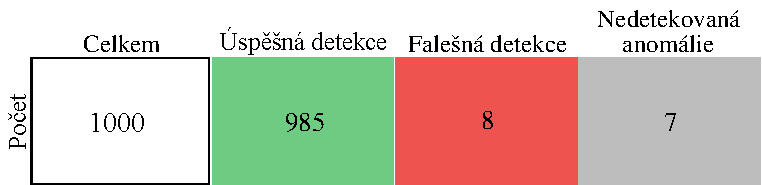
\includegraphics[width=0.83\textwidth]{obrazky/result-matrix.pdf}
    \caption{Číselné výsledky testu detekce anomálií nad náhodnými datasety}
    \label{matice-vysledku-img}
\end{figure}

V~8 datasetech došlo k~falešné detekci anomálie. Celkem 5 případů spočívalo v~klasifikaci přirozených outlierů jako anomálie. Ve zbylých 3 byly za~anomálie považovány shluky jako na~obrázku~\ref{chybne-nalezena-anomalie-img}.

\begin{figure}[hbt]
    \centering
    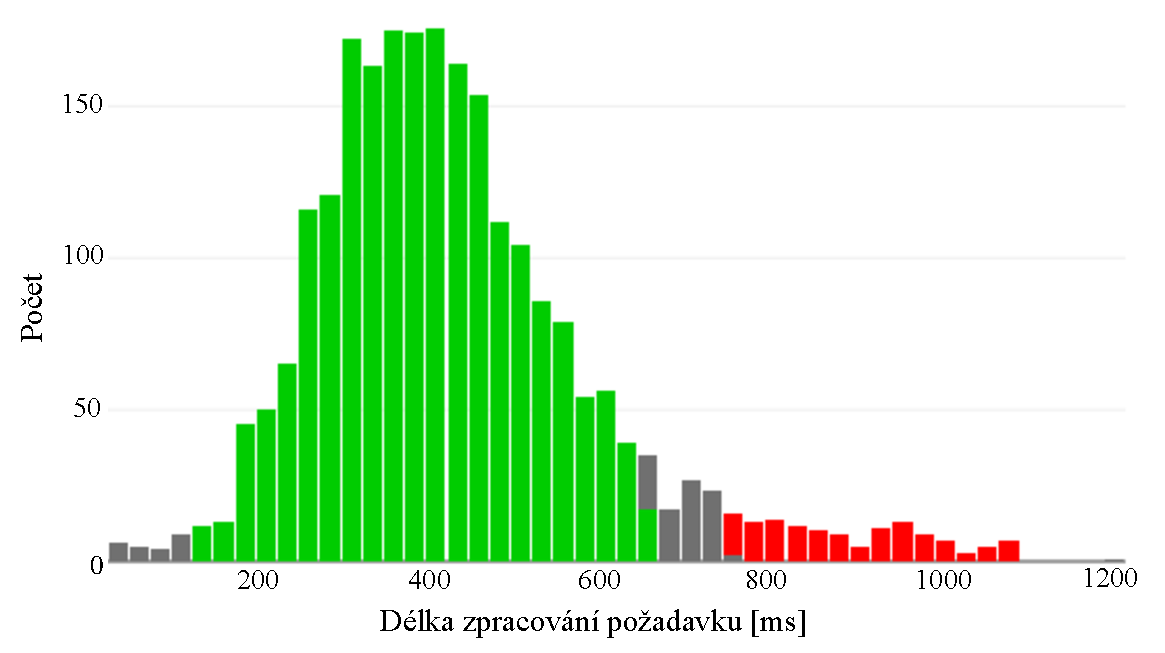
\includegraphics[width=0.9\textwidth]{obrazky/testovani-false-anomaly.pdf}
    \caption{V~těchto datech se chybně nalezla anomálie. Outliery byly zřejmě dostatečně blízko sebe na~vytvoření širokého, řídkého a rovnoměrného shluku, jenž se však v~celkovém kontextu anomálně nechová.}
    \label{chybne-nalezena-anomalie-img}
\end{figure}

Pouze v~7 případech se anomálii nepodařilo detekovat. Jen ve~4 z~nich však byla anomálie naprosto zřetelná. V~ostatních se jednalo o~sporné situace podobné obrázku~\ref{nenalezena-anomalie-img}, kde je spíše věcí názoru, jestli by se o~anomálii jednat mělo, či ještě ne.

\begin{figure}[!hbt]
    \centering
    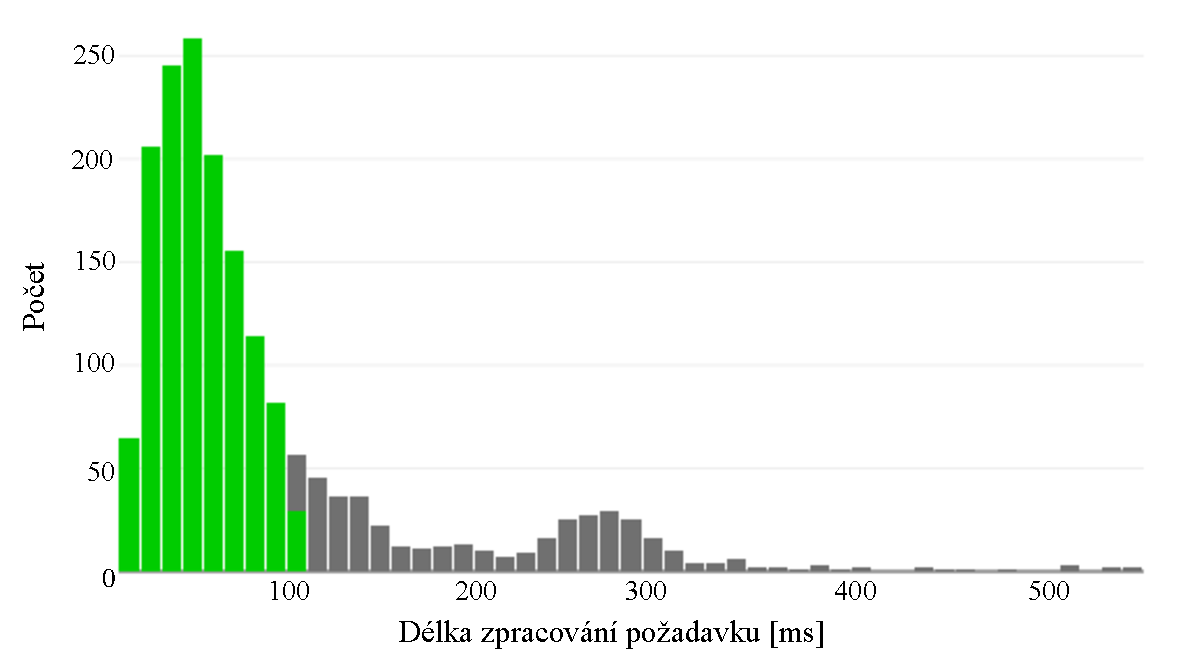
\includegraphics[width=0.9\textwidth]{obrazky/testovani-unrecognized-anomaly.pdf}
    \caption{Výkyv v~datech nebyl rozpoznán jako anomálie.}
    \label{nenalezena-anomalie-img}
\end{figure}

Dále se při~úspěšné detekci 9krát stalo, že k~sobě anomálie zahrnula i okolní data, jež by do~ní patřit neměla. Toto zobrazuje obrázek~\ref{prilis-siroka-anomalie-img}. Byť se jedná o~nepřesnost, přímo za~chybu se to nepovažuje, neboť anomálie detekována byla a uživatel by již neměl problém si situaci interpretovat.

\begin{figure}[!hbt]
    \centering
    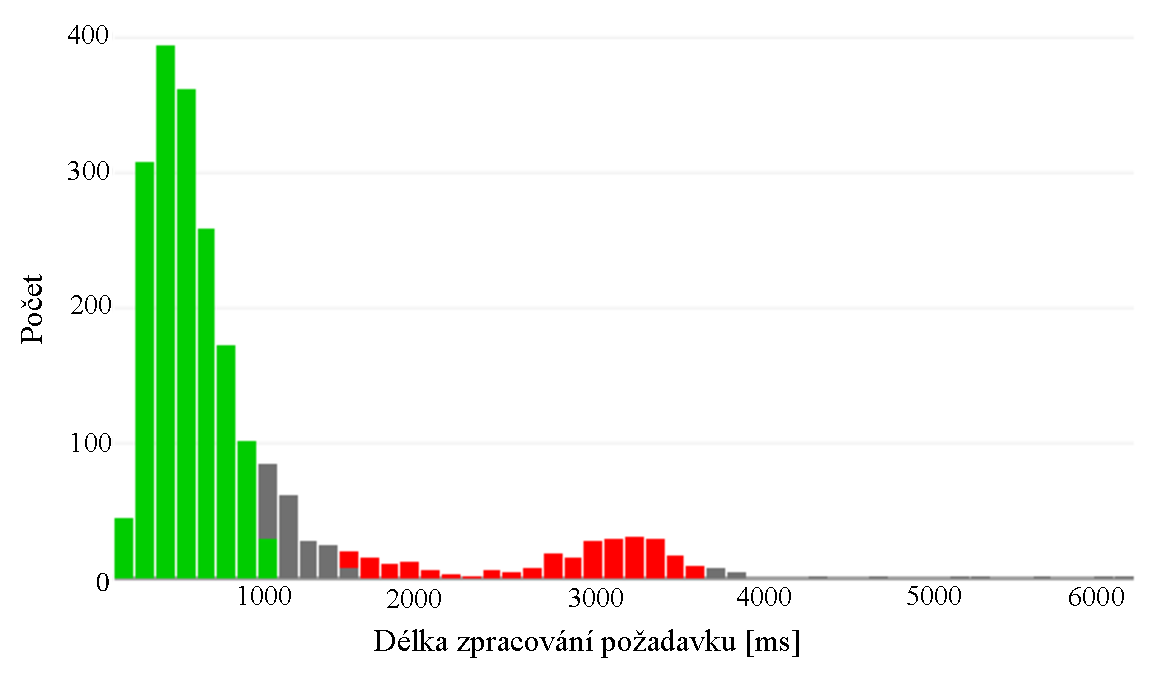
\includegraphics[width=0.9\textwidth]{obrazky/testovani-too-wide-anomaly.pdf}
    \caption{Anomálie obsahuje i okolní data, která již nejsou přímo součástí shluku.}
    \label{prilis-siroka-anomalie-img}
\end{figure}

Výsledek si lze vyložit velmi pozitivně. Celkových~985 správných detekcí z~1000 dělá úspěšnost 98.5~\%, což je velmi uspokojivé. Dále pokud by se bral v~potaz parametr tolerance pro~potlačení anomálií blízko dat, jenž bude v~RQA zcela jistě použit, přirozené outliery by se za~anomálie nikdy neklasifikovaly. To by v~tomto případě zvýšilo počet správných detekcí na~990 a úspěšnost na~99~\%. Kdyby se navíc nebraly v~potaz sporné anomálie, tak~990 správných detekcí z~997 dělá úspěšnost zaokrouhleně~99.3~\%.

\section{Testování detekce anomálií v~chybovosti požadavků}
Testování této funkcionality se ukázalo být celkem jednoduché. Vzhledem k~tomu, že se jedná pouze o~porovnání poměrů počtů chyb mezi dvěma datasety, stačilo ověřit jen několik specifických případů. Nejprve se vytvořil referenční dataset obsahující~70~\% požadavků bez chyb,~20~\% s~1 chybou a zbylých~10~\% se~2 chybami. Dále se testovalo, zda-li se anomálie detekuje, bude-li vše v~mezích. Vygenerovalo se několik datasetů takovým způsobem, aby nebyl nikdy nepřekročen rozdíl~10~\% u~některého počtu chyb, tedy s~60-80~\% požadavků bez chyb,~10-30~\% s~1 chybou a~0-20~\% se~2 chybami. Anomálie nebyla nikdy detekována.

Dále se testovaly anomální situace. První je překročení dané meze. Vygenerovaly se tedy datasety obsahující více než~80~\% nebo méně než~60~\% požadavků bez chyb a podobně i u~ostatních počtů chyb. Druhým typem anomálie je doposud neviděný počet chyb. Proto byly vytvořeny datasety s~požadavky se~3 i více chybami, ať už v~rámci anomální meze, nebo ne. V~obou případech se jedná o~anomálii. Všechny požadované anomální stavy byly rozeznány.

\section{Vyhodnocení dosažených výsledků}
Na~základě výsledků testů sekce~\ref{testovani-delka-pozadavku} lze dospět k~závěru, že detekce anomálií v~délkách zpracování požadavků funguje velmi dobře. Úspěšnost přesahující 98~\% je toho zjevným důkazem. Těchto výsledků bylo dosaženo i navzdory požadavku na~obecnost detekce. Řešení navíc není zcela uzavřené a umožňuje uživateli nastavovat toleranci pro~anomálie, ať už v~její velikosti nebo pozici.

Návrh detekce s~ohledem na~obecnost dat však nepopiratelně zapříčiňuje nepřesnosti. Jednou z~nich je nespolehlivé rozpoznání okrajů platných dat, čímž se z~nich již stávají outliery. Další je, že anomální shluky občas neobsahují vše, co by měly, nebo naopak mají přesah do~dat, jež by do~nich již patřit neměly. Někdy zase obecné parametry nedostačují pro~kvalitní shlukování a anomálii se nepodaří detekovat. S~rostoucími požadavky na~obecnost klesá přesnost, a~proto je řešení kompromisem, jenž se části přesnosti musel vzdát.

Detekce anomálií v~chybách během požadavků nevyužívá žádné specifické algoritmy strojového učení, nýbrž jen statistické výpočty. Bude tedy vždy vykazovat stejné výsledky dle definovaných parametrů. Všechny specifikované anomální případy dokáže rozpoznat, a~tak jestli nedojde k~nepředpokládané situaci, bude vždy pracovat správně.

Výsledky jsou pozitivně vnímány i firmou Y~Soft, jejíž posudek je přiložen v~příloze~\ref{priloha-D}. Způsob provedení i funkčnost plně splňují jejich požadavky. Z~technického hlediska jsou spokojeni především se snadným zahrnutím mikroslužeb do~detekce anomálií pomocí instalace rozšíření a implementací na~platformě .NET.
  \chapter*{Závěr}
\addcontentsline{toc}{chapter}{Závěr} 

Práce představila robotický systém RQA pro~automatizaci testování zařízení a vysvětlila nutnost detekce anomálií v~požadavcích na~mikroslužby, jež tento systém tvoří. Anomálie se konkrétně hledaly mezi délkami zpracování jednotlivých požadavků a v~jejich chybovosti.

Byl navržen a implementován sběr dat potřebných pro~detekci anomálií. Data jsou zaznamenávána pomocí mechanismu middleware a ukládána formou logů v~centrálním logovacím systému Graylog. Logy nesou identifikační údaje, jimiž jsou časové razítko, jméno cílové služby a její obslužné rutiny. Dále obsahují samotné údaje pro~detekci, tedy úroveň závažnosti pro~určení chyby a délku zpracování požadavku, jedná-li se o~log oznamující konec požadavku. Z~Graylogu jsou data stahována a transformována do~formátu CSV, jenž se ukládá na straně aplikace provádějící jejich následnou analýzu.

Byla provedena rešerše algoritmů strojového učení bez učitele pro~detekci anomálií se~zaměřením na~shlukovou analýzu. Práce pro~úplnost popisuje představitele všech základních kategorií shlukových algoritmů navzdory tomu, že některé kategorie jako takové nejsou vhodné pro~zadaný úkol. Mimo shlukovou analýzu práce představuje i zástupce rozhodovacích stromů nebo statistických metod.

Anomálie v~délkách zpracování požadavků se definovala jako shluk outlierů, a~proto jejich detekce probíhá ve~dvou průchodech. V~prvním se oddělí platná data od~outlierů kombinací shlukového algoritmu založeném na~hustotě DBSCAN a statistické metody modifikovaného z-skóre. V~druhém průchodu se nalezené outliery shlukují algoritmy DBSCAN či HDBSCAN opět s~pomocí modifikovaného z-skóre. Detekce je proveditelná jak na~samostatných datech, tak lze i platná data předchozích detekcí použít jako referenční dataset pro~následné detekce.

Analýza chybových požadavků již nevyužívá strojové učení, nýbrž pouze statisticky porovnává poměry počtů chyb během požadavků mezi referenčními a nově příchozími daty. Za~anomálii je prohlášen stav, kdy se tyto poměry liší o~více než stanovenou mez.

Výsledné řešení odpovídá požadavkům firmy Y~Soft na~detekci anomálií v~RQA. Dokáže pracovat nad~různými typy požadavků služeb s~odlišnými vlastnostmi a navzdory této obecnosti velmi úspěšně. Dalším postupem bude jeho integrace do~systému RQA, monitorování výsledků detekce v~reálném provozu a ladění parametrů použitých algoritmů pro~ještě další zpřesnění.
  
  % Kompilace po částech (viz výše, nutno odkomentovat)
  % Compilation piecewise (see above, it is necessary to uncomment it)
  %\subfile{projekt-01-uvod-introduction}
  % ...
  %\subfile{chapters/projekt-05-conclusion}


  % Pouzita literatura / Bibliography
  % ----------------------------------------------
\ifslovak
  \makeatletter
  \def\@openbib@code{\addcontentsline{toc}{chapter}{Literatúra}}
  \makeatother
  \bibliographystyle{bib-styles/Pysny/skplain}
\else
  \ifczech
    \makeatletter
    \def\@openbib@code{\addcontentsline{toc}{chapter}{Literatura}}
    \makeatother
    \bibliographystyle{bib-styles/Pysny/czplain}
  \else 
    \makeatletter
    \def\@openbib@code{\addcontentsline{toc}{chapter}{Bibliography}}
    \makeatother
    \bibliographystyle{bib-styles/Pysny/enplain}
  %  \bibliographystyle{alpha}
  \fi
\fi
  \begin{flushleft}
  \bibliography{08-Literatura}
  \end{flushleft}

  % vynechani stranky v oboustrannem rezimu
  % Skip the page in the two-sided mode
  \iftwoside
    \cleardoublepage
  \fi

  % Prilohy / Appendices
  % ---------------------------------------------
  \appendix
\ifczech
  \renewcommand{\appendixpagename}{Přílohy}
  \renewcommand{\appendixtocname}{Přílohy}
  \renewcommand{\appendixname}{Příloha}
\fi
\ifslovak
  \renewcommand{\appendixpagename}{Prílohy}
  \renewcommand{\appendixtocname}{Prílohy}
  \renewcommand{\appendixname}{Príloha}
\fi
%  \appendixpage

% vynechani stranky v oboustrannem rezimu
% Skip the page in the two-sided mode
%\iftwoside
%  \cleardoublepage
%\fi
  
\ifslovak
%  \section*{Zoznam príloh}
%  \addcontentsline{toc}{section}{Zoznam príloh}
\else
  \ifczech
%    \section*{Seznam příloh}
%    \addcontentsline{toc}{section}{Seznam příloh}
  \else
%    \section*{List of Appendices}
%    \addcontentsline{toc}{section}{List of Appendices}
  \fi
\fi
  \startcontents[chapters]
  \setlength{\parskip}{0pt} 
  % seznam příloh / list of appendices
  % \printcontents[chapters]{l}{0}{\setcounter{tocdepth}{2}}
  
  \ifODSAZ
    \setlength{\parskip}{0.5\bigskipamount}
  \else
    \setlength{\parskip}{0pt}
  \fi
  
  % vynechani stranky v oboustrannem rezimu
  \iftwoside
    \cleardoublepage
  \fi
  
  % Přílohy / Appendices
  \chapter{Slovník pojmů}
\label{priloha-A}

\renewcommand*{\arraystretch}{1.4}
\begin{longtable}{p{3cm}p{11.2cm}}
Backend & Část aplikace obsahující její logiku. Typicky běží na~serveru a uživatel do~ní nevidí.\\

Klient & Aplikace běžící na~straně uživatele.\\

Kontrolér & V~kontextu webového api přijímá požadavky na~službu a vrací odpovědi. Akce kontroléru k~vykonání je specifikována v~url požadavku.\\

Kubernetes & Open-source platforma pro~správu a nasazení kontejnerizovaných aplikací.\\

Dataframe & Dvou-dimenzionální datová struktura tabulkového stylu s~pojmenovanými sloupci.\\

Dataset & Kolekce dat, nad~kterými se vykonává analýza.\\

Framework & Software, který obsahuje a poskytuje pomocné prvky k~vývoji nových aplikací.\\

Log & Záznam o~činnost.\\

Logger & Objekt implementující ILogger rozhraní schopný vytvářet logy.\\

NuGet & Instalační balíček knihovny či rozšíření pro~.NET projekty.\\

Open-source & Software, který bývá typicky zdarma a jehož zdrojové kódy jsou veřejně dostupné.\\

Outlier & Hodnota výrazně se lišící od~ostatních v~dané kolekci dat.\\

RabitMQ & Open-source software zprostředkovávající zprávy mezi částmi distribuovaných systémů.\\

Routing & V~kontextu webového API se jedná o~směrování požadavků. Mapuje požadavky na~konkrétní kontroléry a jejich akce.\\

Výjimka & V~kontextu programování se jedná o~výjimečnou situaci, typicky chybu. \\

Widget & Ovladatelný prvek grafického uživatelského rozhraní.\\

XPlot & Vizualizační knihovna pro~jazyk F\#, který lze díky kompatibilitě .NET platformy omezeně použít i v~C\#.
\end{longtable}

\chapter{Seznam zkratek}
\label{priloha-B}

\renewcommand*{\arraystretch}{1.4}
\begin{longtable}{p{2cm}p{12.2cm}}
API & Application Programming Interface (Rozhraní pro~programování aplikací)\newline
Rozhraní, jež umožňuje používat funkce nebo části softwarového systému.\\

CSV & Comma Separated Values (Hodnoty oddělené čárkou)\newline
Typ datového souboru, ve~kterém je na~každém řádku jeden záznam, jehož hodnoty jsou odděleny čárkou.\\

DBSCAN & Density based spatial clustering of applications with noise\newline
Shlukovací algoritmus strojového učení.\\

DI & Dependency Injection (Vkládání závislostí)\newline
Návrhový vzor pro~získávání objektů jinému objektu, na~kterých tento závisí.\\

GELF & Graylog Extended Log Format (Rozšířený formát logů Graylogu)\newline
Logovací poskytovatel pro~Graylog.\\

GMM & Gaussian Mixture Model (Směs Gaussových rozložení)\newline
Shlukovací a klasifikační algoritmus strojového učení.\\

HDBSCAN & Hierarchical density based spatial clustering of applications with noise\newline
Shlukovací algoritmus strojového učení.\\

JSON & JavaScript Object Notation (Objektová notace jazyka JavaScript)\newline
Formát pro serializaci a přenos dat.\\

MinPts & Minimum points (Minimální počet bodů)\newline
Parametr algoritmu DBSCAN určující minimální počet bodů, od~kterého se prostor považuje za~hustý.\\

MRD & Mutual Reachability Distance (Vzdálenost vzájemné dosažitelnosti)\newline
Typ vzdálenosti používající se algoritmem HDBSCAN.\\

OPTICS & Ordering Points to Identify Cluster Structure\newline
Shlukovací algoritmus strojového učení.\\

RD & Reachability Distance (Vzdálenost dosažitelnosti)\newline
Typ vzdálenosti používající se algoritmem OPTICS.\\

REST & Representational State Transfer (Přenost reprezentativního stavu)\newline
Typ architektury využívaný pro webové služby.\\

ROI & Return of Investment (Návratnost investice)\newline
Poměr zisku a investice.\\

RPA & Robotic Process Automation (Robotická automatizace procesů)\newline
Jedná se o~provádění akcí tzv. boty nebo-li softwarovými roboty za~účelem automatizace.\\

RQA & Robotic Quality Assurance (Robotické zajištění jakosti)\newline
Systém firmy Y~Soft pro~robotické automatizované testování.\\

SOM & Self-Organizing Maps\newline
Shlukovací algoritmus strojového učení.\\
   
QA & Quality Assurance (Zajištění jakosti)\newline
Obor zabývající se plánováním a vylepšováním procesů.\\

UI & User Interface (Uživatelské rozhraní)\newline
Část aplikace určená pro~interakci člověka s~počítačem.\\
   
\end{longtable}

\chapter{Vývojový diagram dávkového stahování logů z~Graylogu}
\label{priloha-C}

\begin{figure}[tbh]
	\centering
	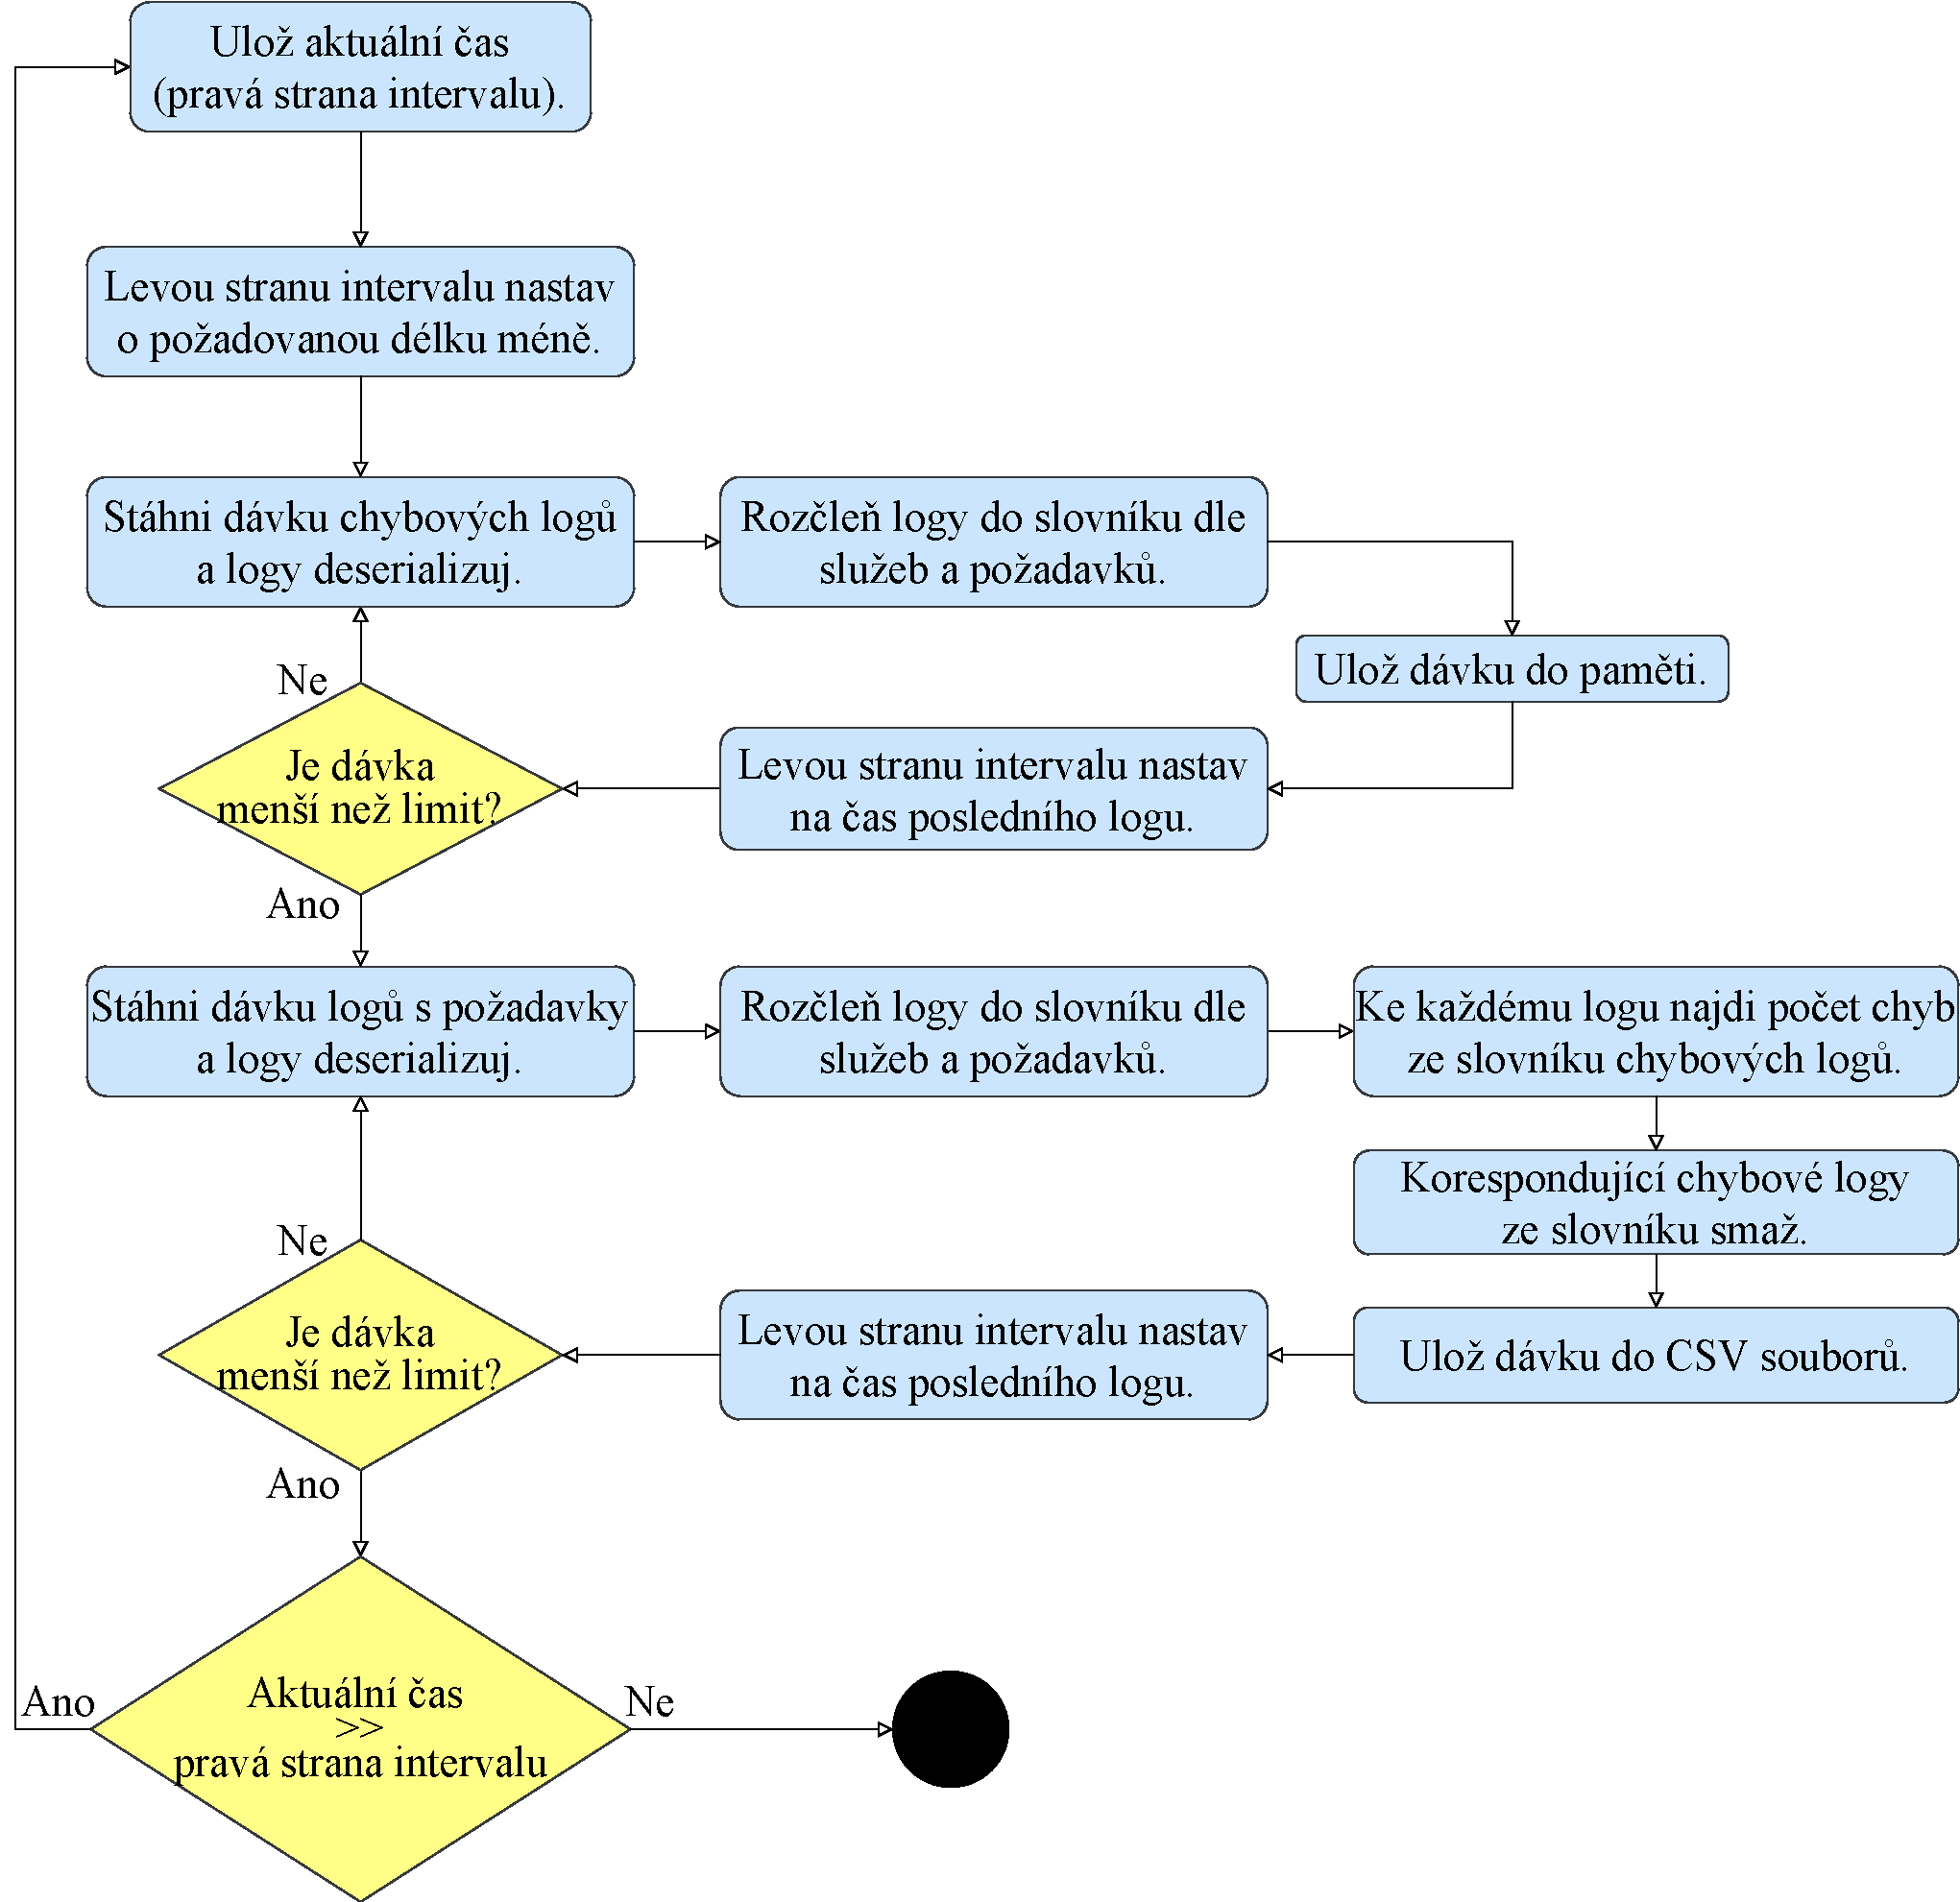
\includegraphics[width=0.97\textwidth]{obrazky/graylog-download-algorithm.pdf}
	\caption{Algoritmus dávkového stahování logů z~Graylogu}
\end{figure}

\chapter{Posudek firmy Y~Soft na~řešení detekce anomálií}
\label{priloha-D}
\begin{figure}[tbh]
	\centering
	
\includegraphics[width=1\textwidth]{obrazky/posudek-ysoft.pdf}
	\caption{Posudek firmy Y~Soft na~řešení detekce anomálií}
\end{figure}

\chapter{Obsah přiloženého paměťového média}
\label{priloha-E}

\begin{itemize}
  \item \texttt{/build} --- Přeložené řešení
  \item \texttt{/demo} --- Jupyter notebooky s~demonstrací řešení
    \begin{itemize}
        \item \texttt{/csv\_examples} --- Ukázkové CSV soubory s~vygenerovanými daty
    \end{itemize}
  \item \texttt{/doc} --- Dokumentace k~řešení
    \begin{itemize}
        \item \texttt{/latex} --- Zdrojové soubory technické zprávy
        \item \texttt{technicka\_zprava.pdf} --- Text bakalářské práce
    \end{itemize}
  \item \texttt{/nuget} --- NuGet balíčky knihoven řešení
  \item \texttt{/src} --- Zdrojové kódy řešení
  \item \texttt{README.md} --- Popis obsahu média a návod k použití
\end{itemize}
  
  % Kompilace po částech (viz výše, nutno odkomentovat)
  % Compilation piecewise (see above, it is necessary to uncomment it)
  %\subfile{projekt-30-prilohy-appendices}
  
\end{document}
